% 34 slides; flexible pacing. Photographs are short pauses in the narrative.
% Pacing and provenance: README.md. No overlays or automatic divider slides.
\part[nopartpage]{Purpose and Programme}

% Slide 1
\begin{frame}{What Should Our Technology Change?}{SDGs in Practice -- Three Years of International Minor Projects}
\begin{columns}[c,onlytextwidth]
\column{.53\textwidth}
\begin{itemize}
    \item \textbf{People and ecosystems} give a project its purpose.
    \item A useful system starts with \textbf{a situation worth improving}.
    \item Three student cohorts show how \textbf{questions become projects}.
\end{itemize}
\vspace{.7em}
\alert{What could become better -- and for whom?}
\column{.43\textwidth}
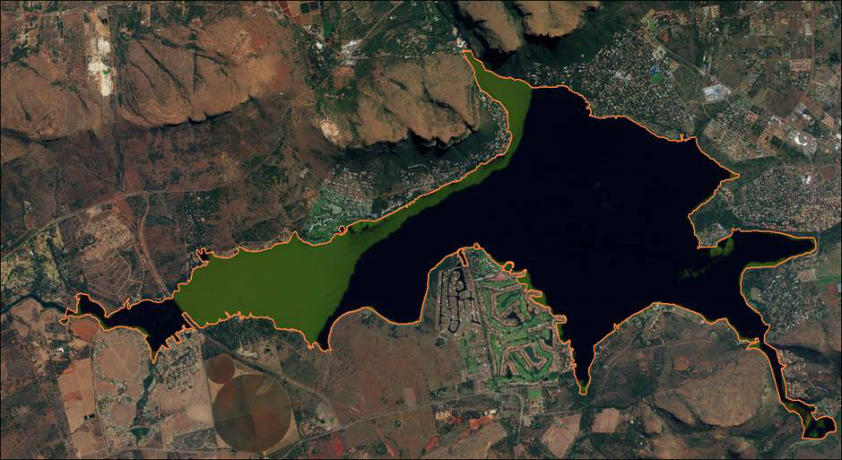
\includegraphics[width=\linewidth,height=.60\paperheight,keepaspectratio]{slides/035-ga-in-it-202425/material/Hartbeespoort-Dam.jpg}
\par\smallskip{\footnotesize Hartbeespoort Dam, South Africa}
\end{columns}
\vfill
{\small Volker Christian \quad$\cdot$\quad FH Upper Austria, Campus Hagenberg}
\end{frame}

% Slide 2
\begin{frame}{International Minor: Global Acting in IT}{One Semester -- Five Countries -- One Shared Project}
\begin{columns}[c,onlytextwidth]
\column{.52\textwidth}
\begin{itemize}
    \item \textbf{International student teams} work on a common challenge.
    \item Five partner universities contribute \textbf{complementary ICT skills}.
    \item Each location adds a perspective; \textbf{the project travels with the team}.
    \item Collaboration connects \textbf{technical learning and societal purpose}.
\end{itemize}
\column{.44\textwidth}
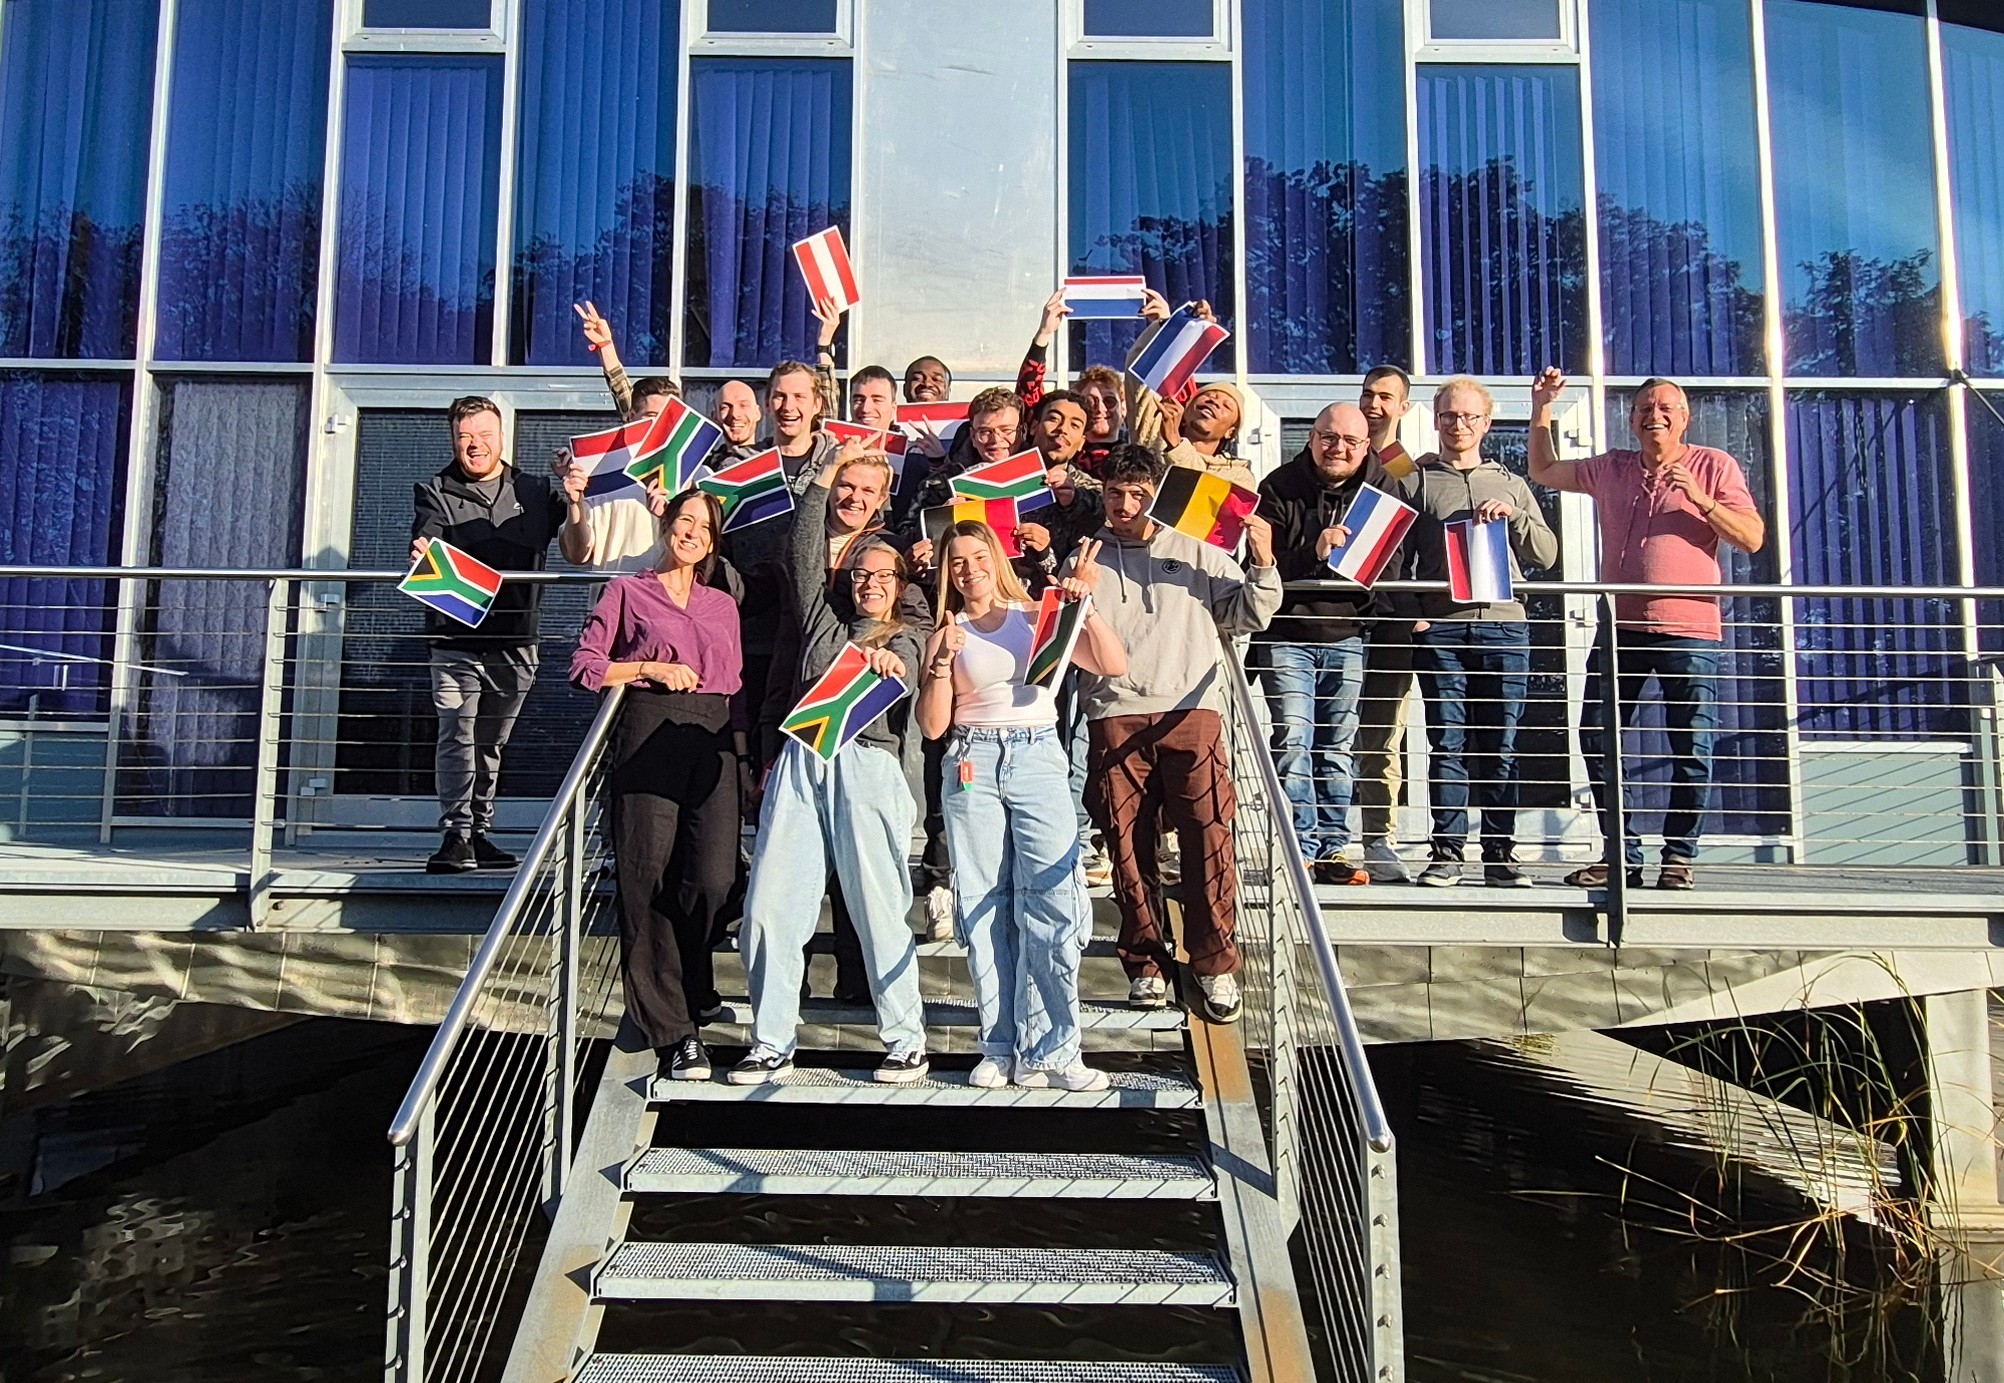
\includegraphics[width=\linewidth,height=.63\paperheight,keepaspectratio]{slides/035-ga-in-it-202425/material/InternationalMinorStudents2024.jpg}
\par\smallskip{\footnotesize The 2024 cohort in Hagenberg}
\end{columns}
\end{frame}

% Slide 3
\begin{frame}{Hagenberg: From Ideas to Something That Works}{Three Weeks of Practical Teamwork}
\begin{columns}[c,onlytextwidth]
\column{.52\textwidth}
\begin{itemize}
    \item \textbf{Investigate} what the project and its users need.
    \item \textbf{Design and build} hardware, software and communication.
    \item \textbf{Test and integrate}: the parts must work together.
    \item The lecturer coaches; \textbf{students make and justify decisions}.
\end{itemize}
\column{.44\textwidth}
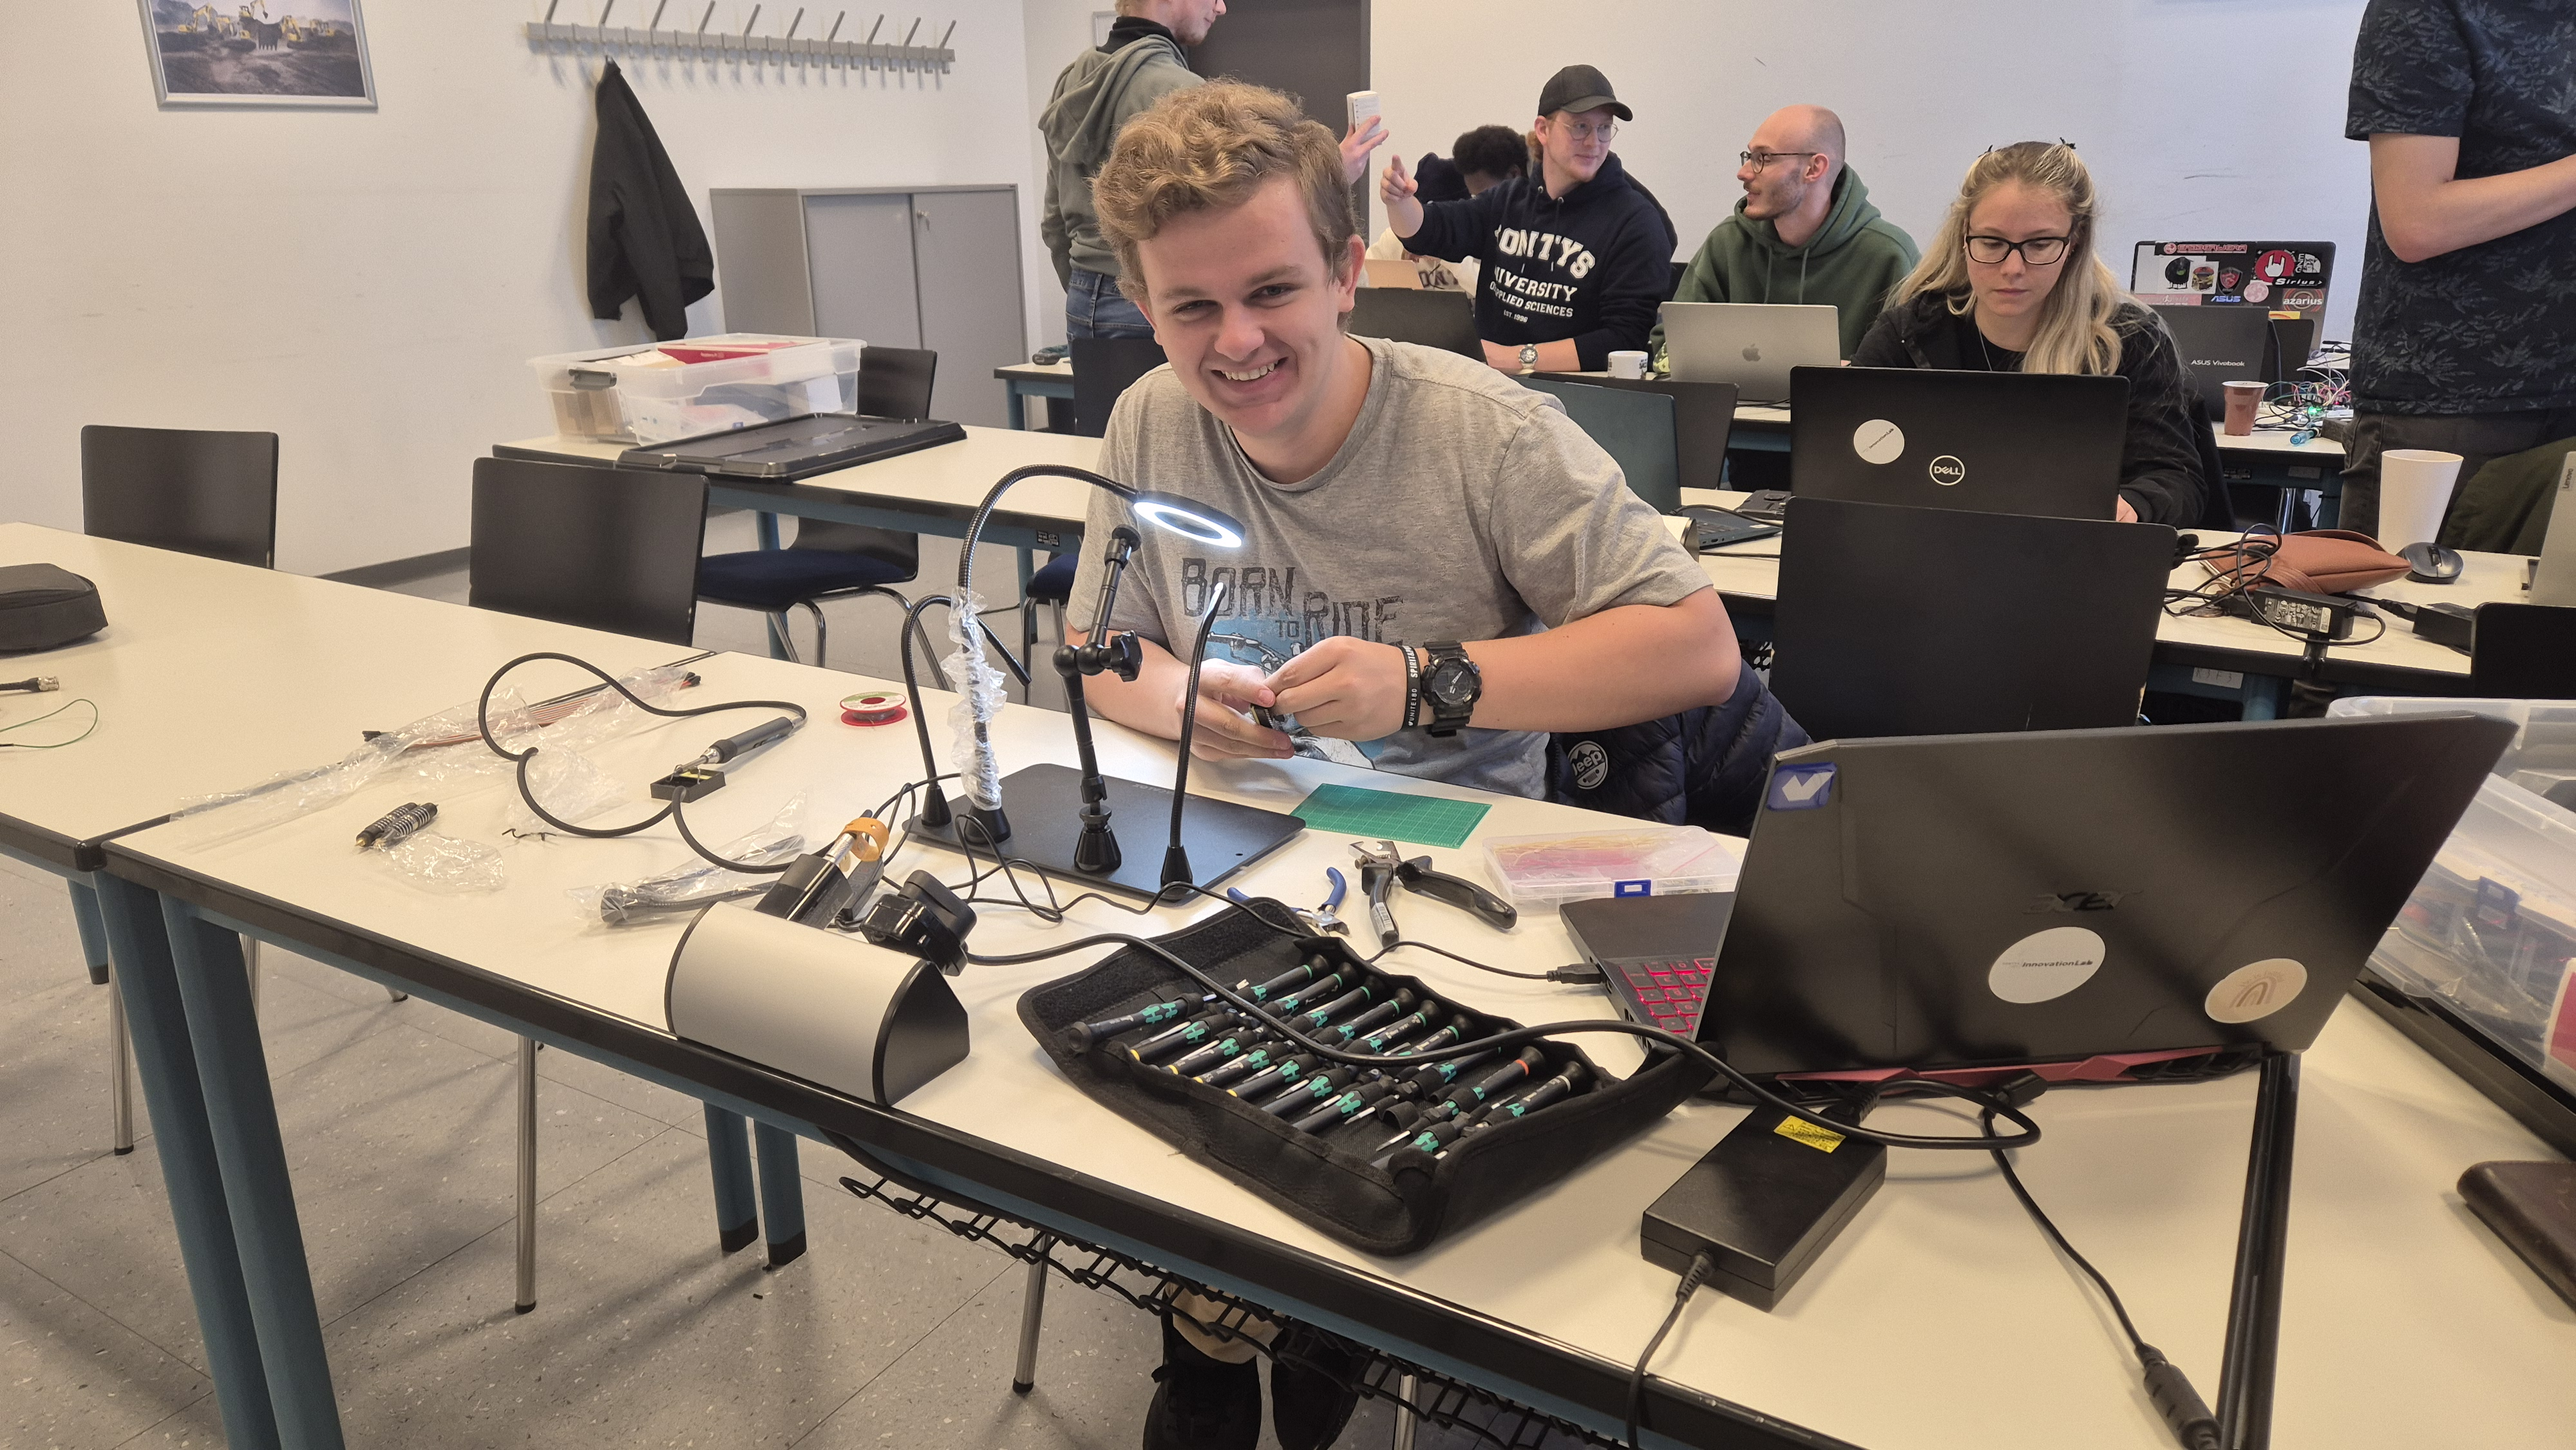
\includegraphics[width=\linewidth,height=.62\paperheight,keepaspectratio]{slides/035-ga-in-it-202425/material/20241104_113440.jpg}
\par\smallskip{\footnotesize Workshop impressions, 2024}
\end{columns}
\end{frame}

\part[nopartpage]{From Goals to Useful Questions}
% Slide 4
\begin{frame}{The SDGs Give Us a Direction}{Global Goals -- Local Contributions}
\begin{itemize}
    \item The \textbf{17 Sustainable Development Goals} connect social, environmental and economic challenges.
    \item Identify a \textbf{specific target and a plausible contribution}, beyond a goal label.
    \item Our projects connect \textbf{ecosystems, invasive species, energy and learning}.
\end{itemize}
\vspace{.6em}
\begin{columns}[T,onlytextwidth]
\column{.23\textwidth}\centering

\includegraphics[height=2cm]{slides/036-sdg-story/material/sdg-icons/goal-06.png}\par\smallskip
{\small Freshwater ecosystems}
\column{.23\textwidth}\centering
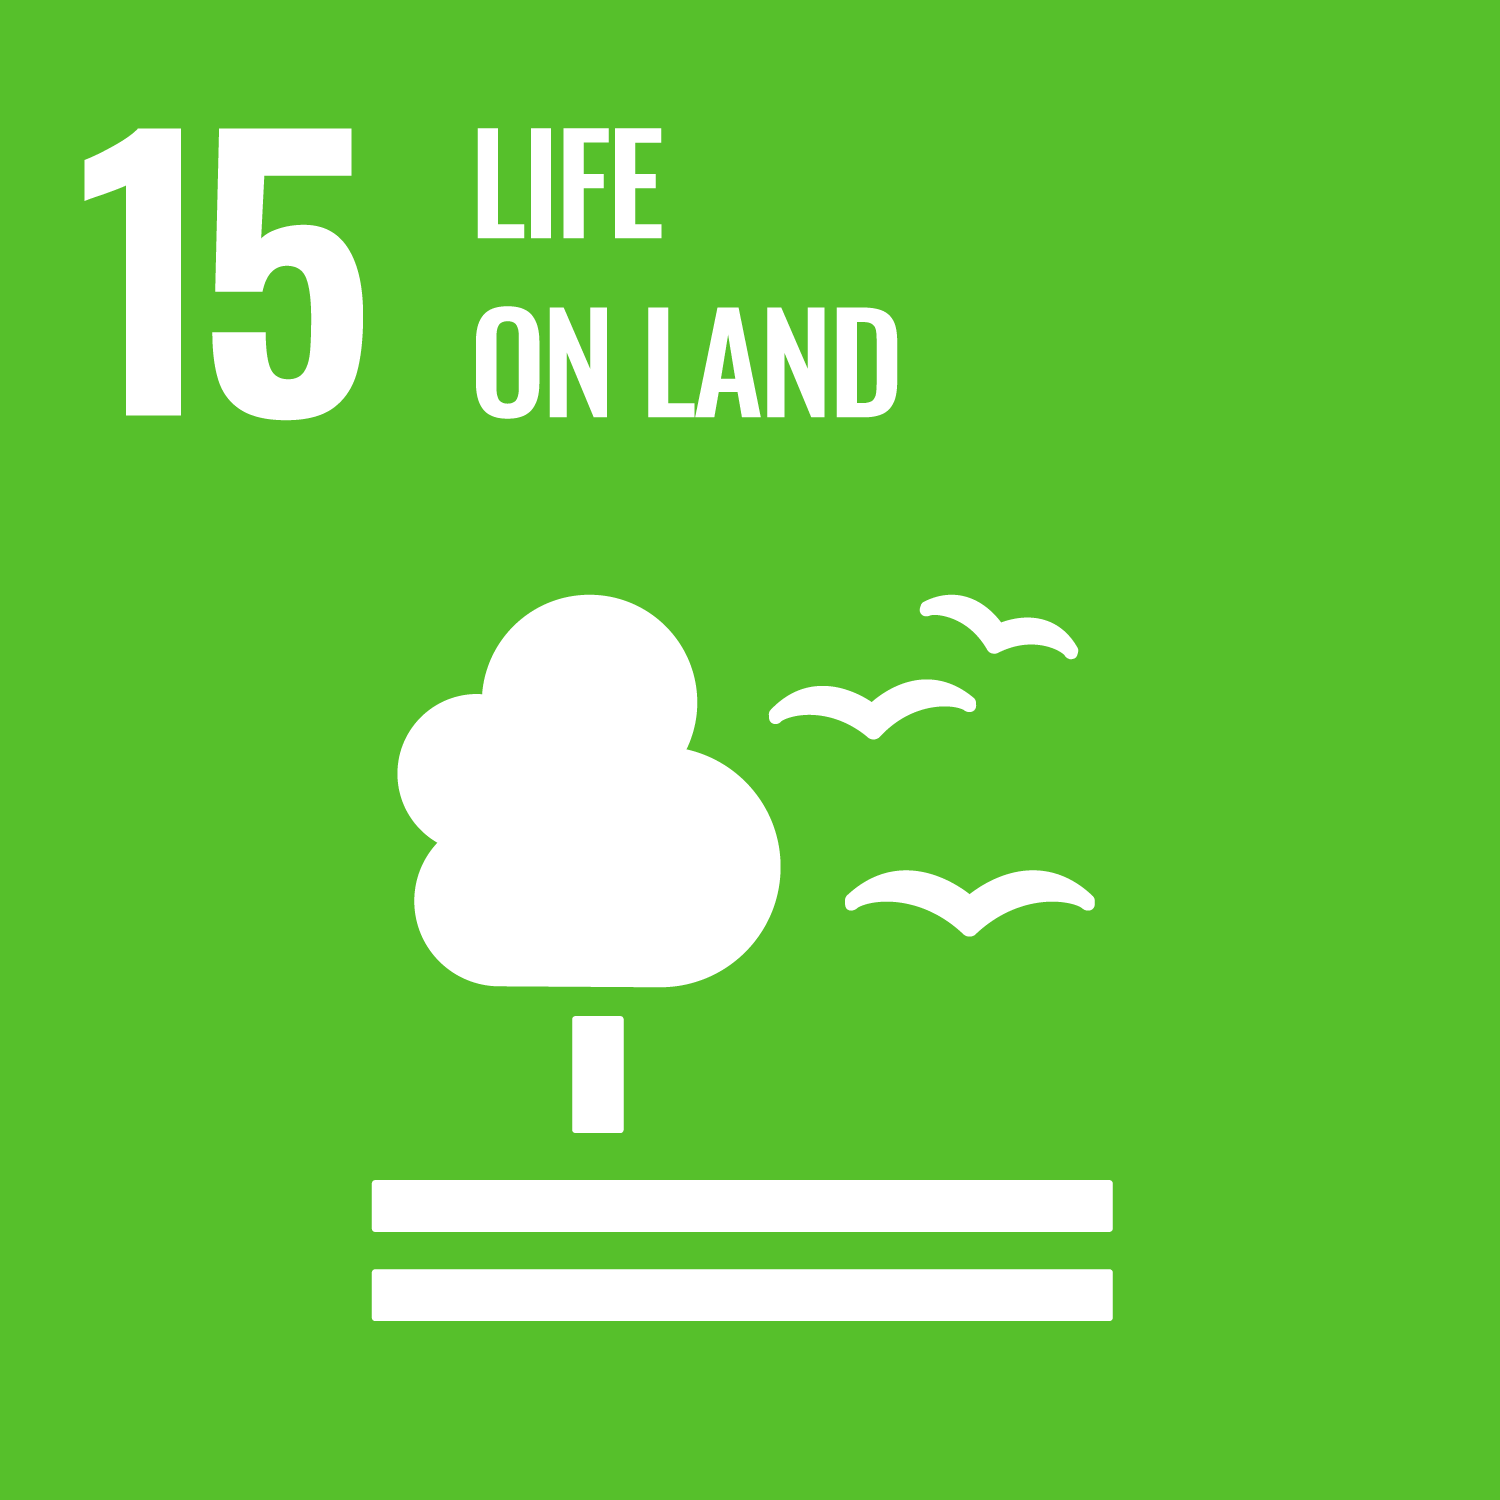
\includegraphics[height=2cm]{slides/036-sdg-story/material/sdg-icons/goal-15.png}\par\smallskip
{\small Invasive species, including in water ecosystems}
\column{.23\textwidth}\centering
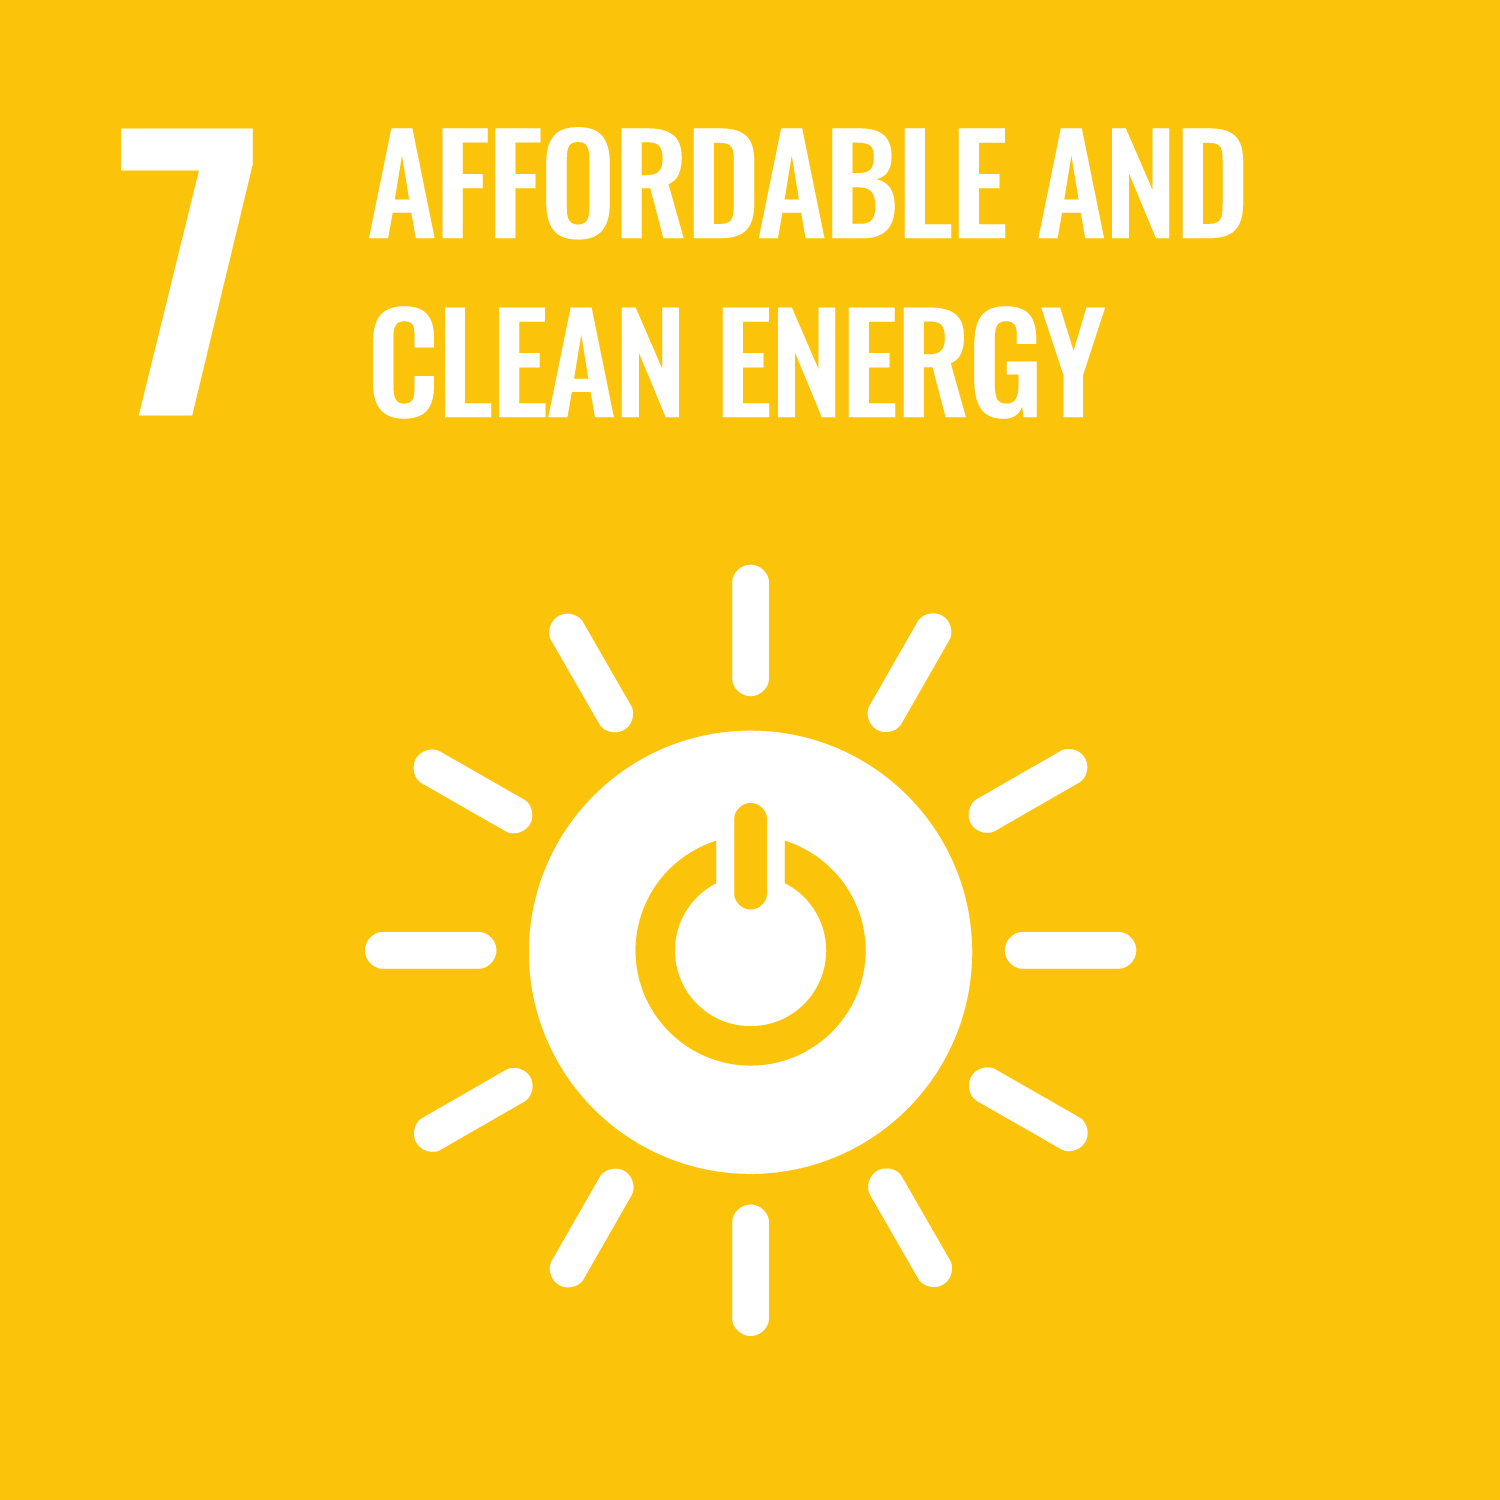
\includegraphics[height=2cm]{slides/036-sdg-story/material/sdg-icons/goal-07.png}\par\smallskip
{\small Renewable energy}
\column{.23\textwidth}\centering

\includegraphics[height=2cm]{slides/036-sdg-story/material/sdg-icons/goal-04.png}\par\smallskip
{\small Learning for sustainable development}
\end{columns}
\vfill
{\scriptsize Official UN icons: \href{https://www.un.org/sustainabledevelopment/}{un.org/sustainabledevelopment}. Project connections describe intended contributions.}
\end{frame}

% Slide 5
\begin{frame}{From a Global Goal to a Local Project}{The Question Comes Before the Tool}
\begin{enumerate}
    \item \textbf{Understand the situation.} What is happening, where, and to whom?
    \item \textbf{Find the missing knowledge.} What would help people make a better decision?
    \item \textbf{Choose a useful intervention.} Observation, learning, action -- or a combination?
    \item \textbf{Select the tools.} IoT can connect physical observations with people and applications.
\end{enumerate}
\vspace{.8em}
\begin{center}
{\large Challenge $\longrightarrow$ Question $\longrightarrow$ Information $\longrightarrow$ Action}
\end{center}
\vspace{.3em}
\alert{A sensor is useful when its measurements serve a purpose.}
\end{frame}

\part[nopartpage]{2024 and 2025 -- Understanding an Ecosystem}
% Slide 6
\begin{frame}{2024: An Ecological Challenge in South Africa}{Invasive Water Plants at Hartbeespoort Dam}
\begin{columns}[c,onlytextwidth]
\column{.52\textwidth}
\begin{itemize}
    \item \textbf{Water hyacinths} are the focus of a real research challenge.
    \item Dense plant cover raises questions about \textbf{water conditions and ecosystem health}.
    \item The \textbf{Centre for Biological Control, Rhodes University}, provides the research context.
    \item First understand \textbf{what researchers need to know}.
\end{itemize}
\column{.44\textwidth}
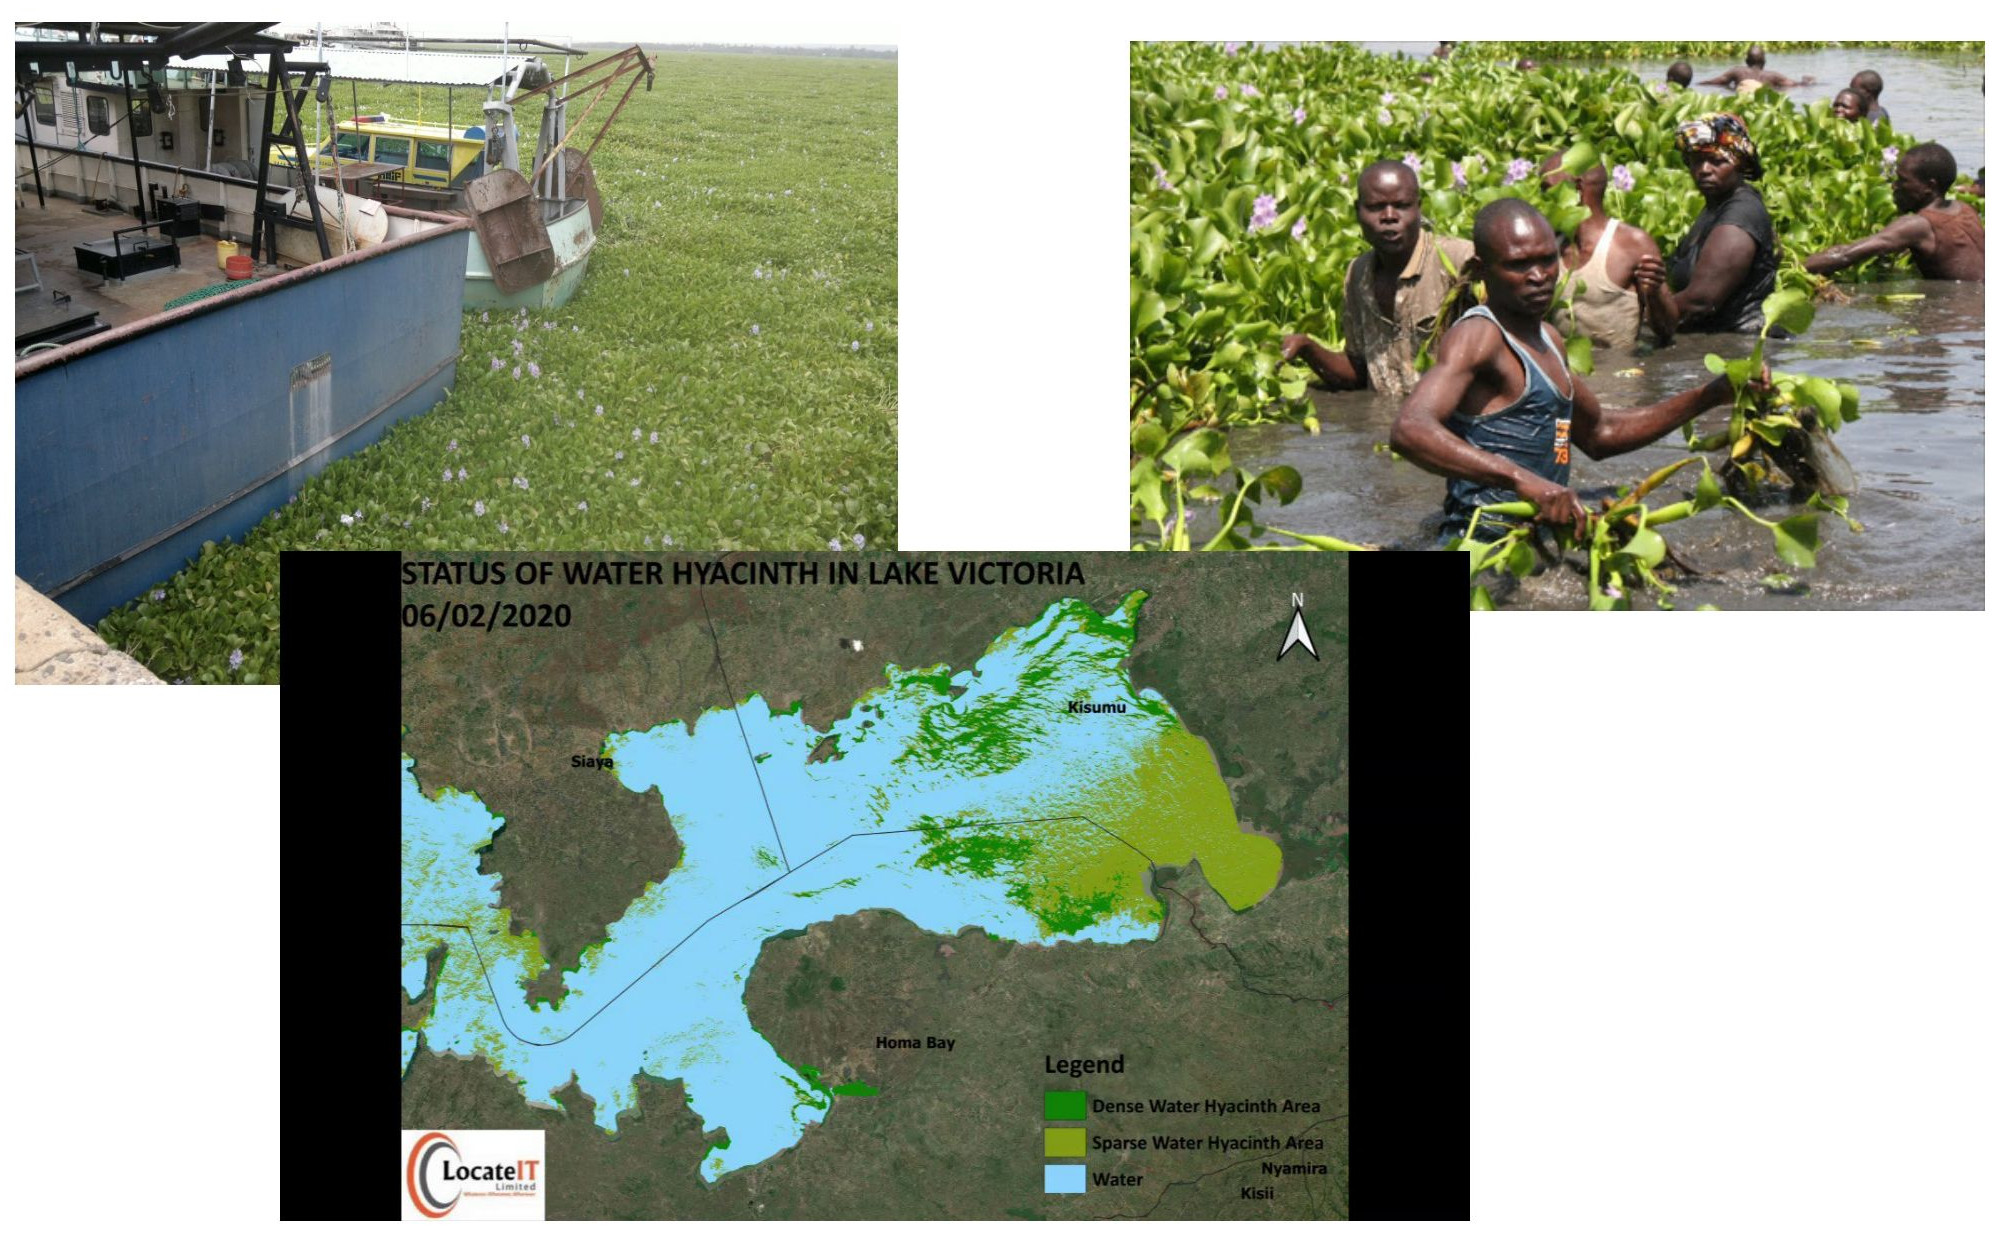
\includegraphics[width=\linewidth,height=.44\paperheight,keepaspectratio]{slides/035-ga-in-it-202425/material/water-hyacinth.jpg}
\par\smallskip\centering

\includegraphics[height=.85cm]{slides/036-sdg-story/material/sdg-icons/goal-06.png}\hspace{.5em}
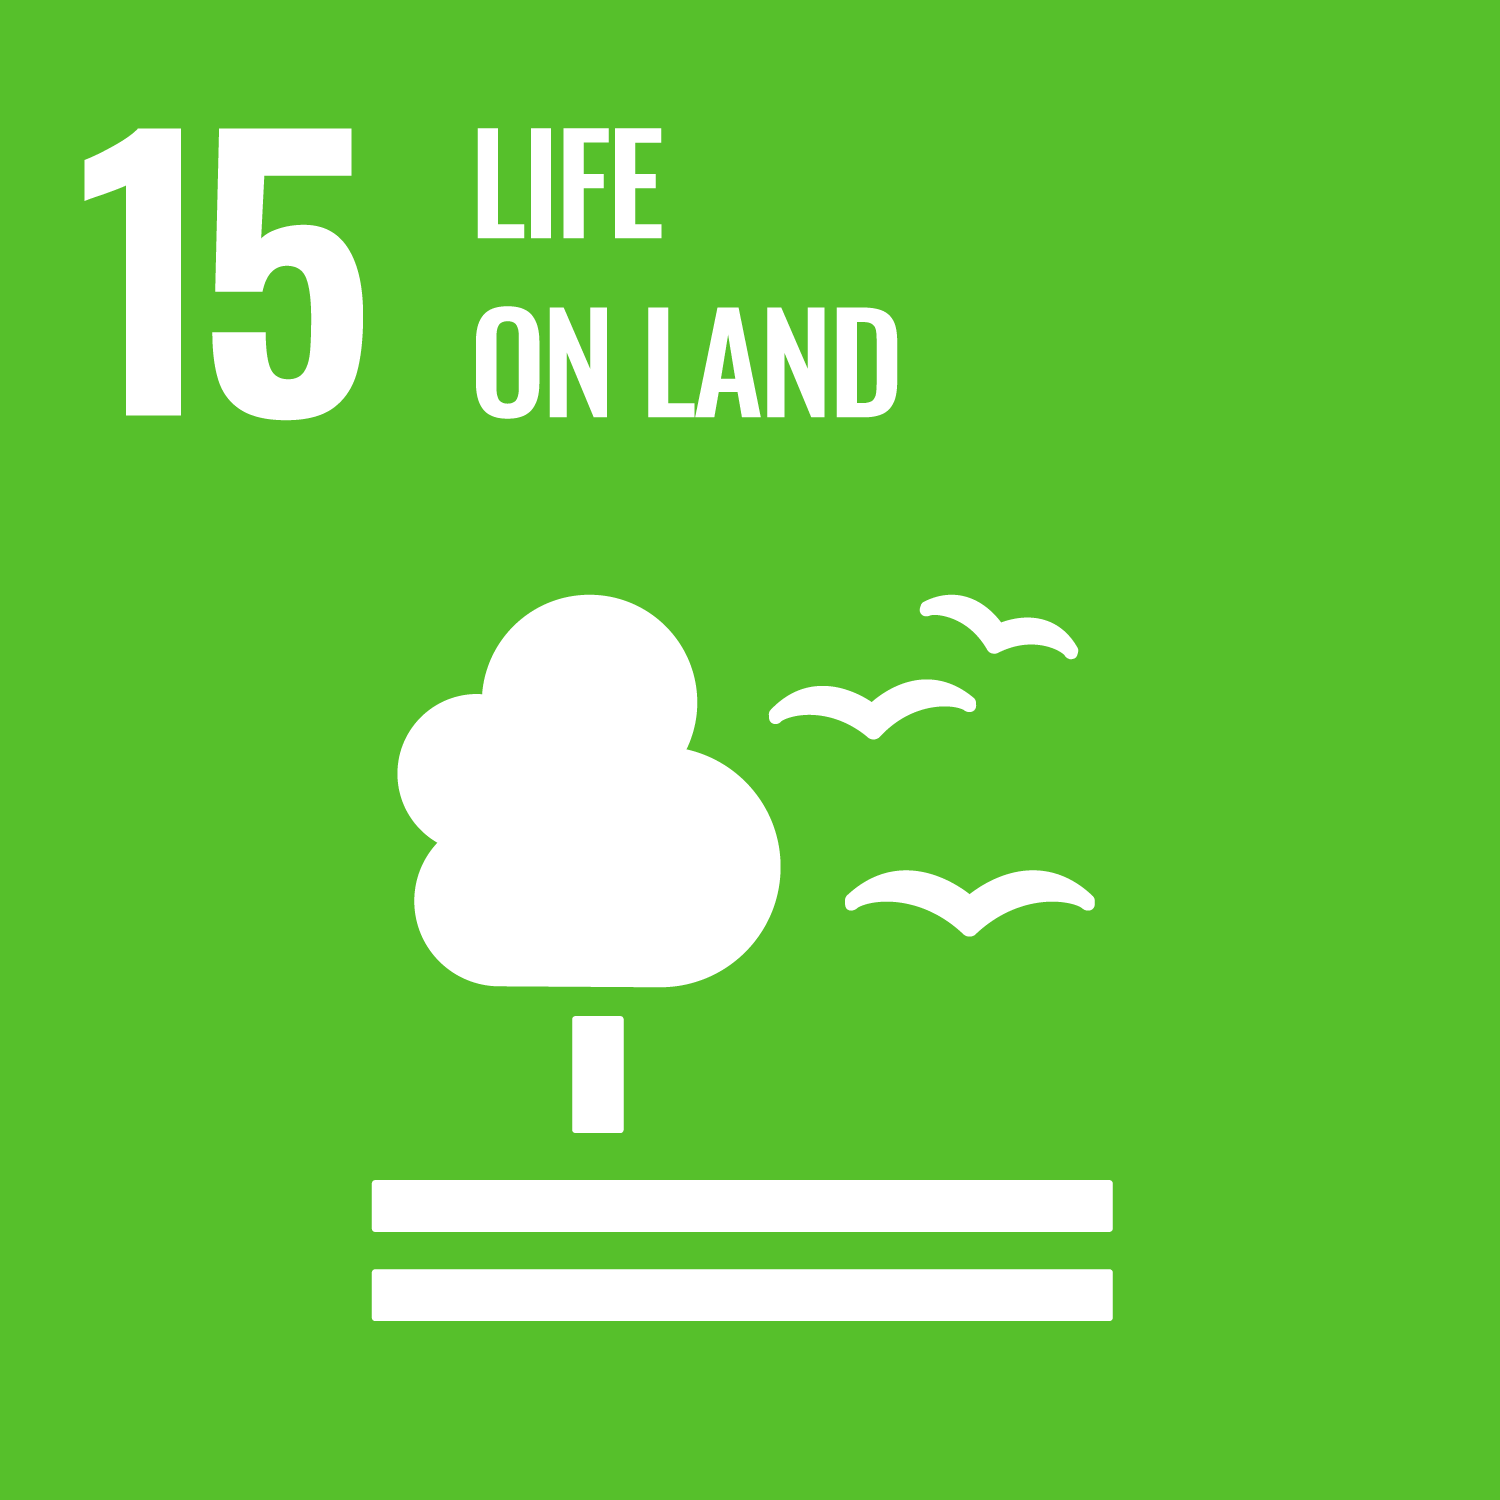
\includegraphics[height=.85cm]{slides/036-sdg-story/material/sdg-icons/goal-15.png}
\end{columns}
\vfill
{\footnotesize \textbf{SDG connection:} freshwater ecosystems (6.6); impacts of invasive species (15.8).\par}
{\scriptsize UN targets: \href{https://sdgs.un.org/goals/goal6}{Goal 6} / \href{https://sdgs.un.org/goals/goal15}{Goal 15}.}
\end{frame}

% Slide 7
\begin{frame}{2024: What Could a Floating Buoy Tell Us?}{Turn an Environmental Question into an Observation}
\begin{columns}[c,onlytextwidth]
\column{.52\textwidth}
\begin{itemize}
    \item Observe \textbf{water conditions over time}, rather than one isolated moment.
    \item Relate measurements to \textbf{location and time}.
    \item The cohort built a \textbf{floating buoy prototype} as a practical response.
    \item Its value depends on \textbf{reliable observations that researchers can interpret}.
\end{itemize}
\column{.44\textwidth}
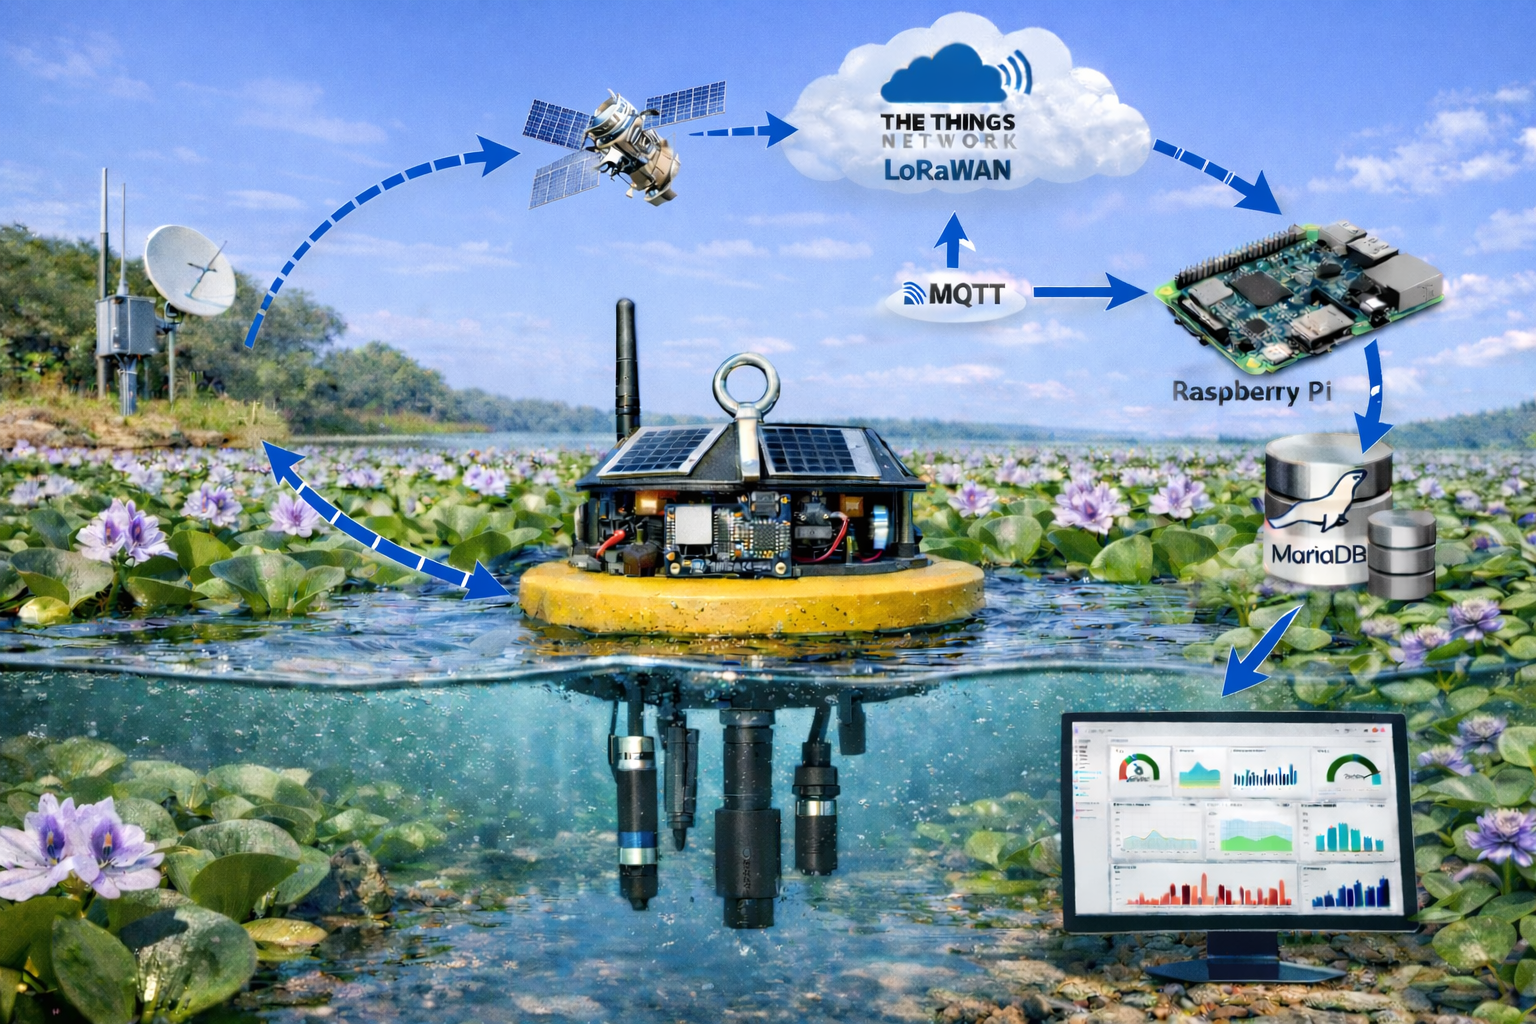
\includegraphics[width=\linewidth,height=.57\paperheight,keepaspectratio]{slides/035-ga-in-it-202425/material/ChatGPT Image Jan 25, 2026, 12_45_31 AM.png}
\par\smallskip{\scriptsize Concept illustration from the existing deck; AI-generated, not a photograph of the prototype.}
\end{columns}
\vfill
\alert{IoT makes the environment observable; people make sense of the observations.}
\end{frame}

% Slide 8
\begin{frame}{The Buoy: Essential Devices}{Real Prototype Electronics -- 2024}
\begin{columns}[c,onlytextwidth]
\column{.37\textwidth}\centering
\begin{tikzpicture}
\node[anchor=south west,inner sep=0] (photo) at (0,0) {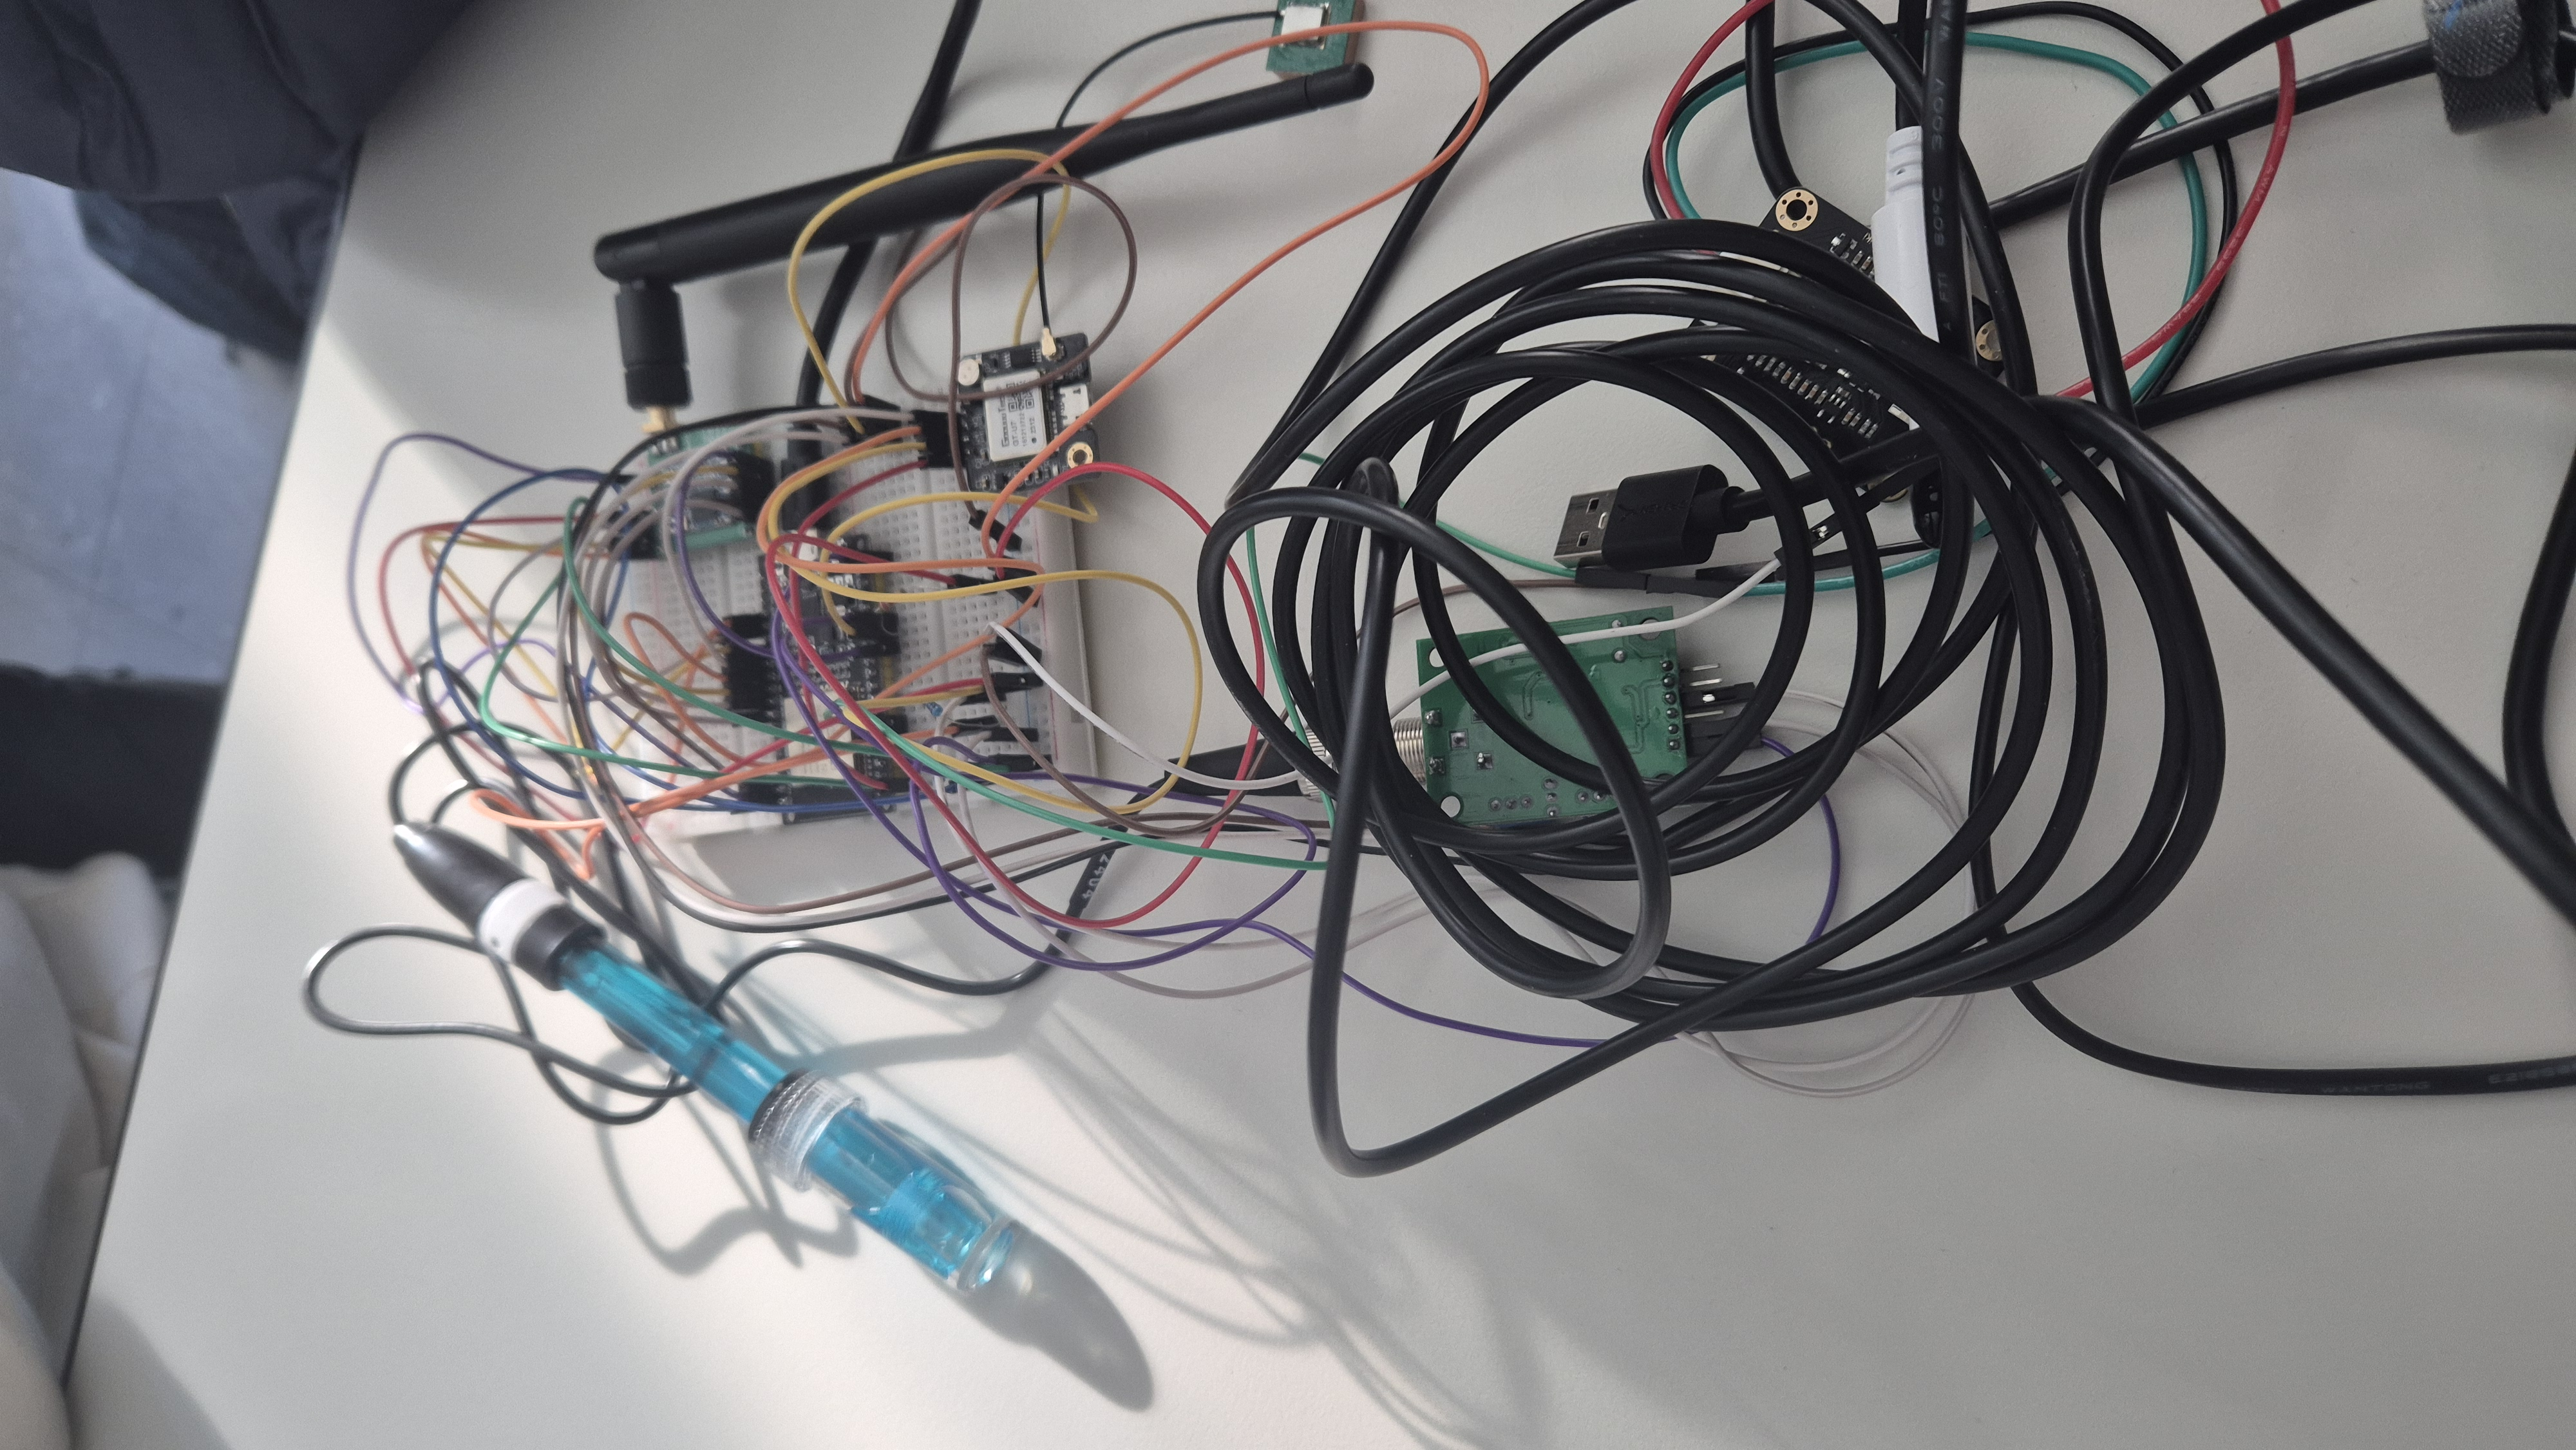
\includegraphics[angle=-90,totalheight=.64\paperheight]{slides/035-ga-in-it-202425/material/20241104_101827.jpg}};
\begin{scope}[x={(photo.south east)},y={(photo.north west)}]
\node[circle,fill=fh-ooe-red,text=white,font=\bfseries\small,inner sep=2pt] at (.50,.68) {1};
\node[circle,fill=fh-ooe-red,text=white,font=\bfseries\small,inner sep=2pt] at (.22,.75) {2};
\node[circle,fill=fh-ooe-red,text=white,font=\bfseries\small,inner sep=2pt] at (.71,.59) {3};
\node[circle,fill=fh-ooe-red,text=white,font=\bfseries\small,inner sep=2pt] at (.88,.53) {4};
\end{scope}
\end{tikzpicture}
\column{.59\textwidth}
\begin{enumerate}
    \item \textbf{MCU}: reads sensors and prepares measurements.
    \item \textbf{pH probe}: one of several water sensors; others observe temperature, turbidity and conductivity/TDS.
    \item \textbf{GPS receiver}: adds location and time.
    \item \textbf{LoRa antenna}: transmits the node's readings.
\end{enumerate}
\vspace{.7em}
\begin{tikzpicture}[every node/.style={align=center,font=\small}]
\node (node) at (0,0) {\textbf{Buoy node}};
\node[draw=fh-ooe-red,text width=2.7cm] (gw) at (4,0) {\textbf{Separate gateway}\\Radio $\rightarrow$ internet};
\draw[->,thick,fh-ooe-red] (node)-- node[above]{LoRaWAN} (gw);
\end{tikzpicture}
\par\smallskip{\small Solar power and storage support operation away from a power socket.}
\end{columns}
\end{frame}



% Slide 9
\begin{frame}{The Buoy: What Each Sensor Contributes}{A Complete Measurement Inventory}
\small\renewcommand{\arraystretch}{1.4}
\par\noindent\begin{tabularx}{\textwidth}{@{}>{\raggedright\arraybackslash}p{.29\textwidth}>{\raggedright\arraybackslash}X@{}}
\toprule
\textbf{Input} & \textbf{What the measurement tells us}\\\midrule
\textbf{pH channel} & Acidity or alkalinity of the water.\\
\textbf{TDS sensor} & An estimate of dissolved solids; a conductivity-related observation, not a direct nutrient measurement.\\
\textbf{Turbidity sensor} & An indication of water cloudiness.\\
\textbf{Water temperature} & The temperature of the water, measured with a DS18B20.\\
\textbf{Board / air temperature} & A separate temperature channel in the pH interface module.\\
\textbf{GPS receiver} & Position and time for relating observations to a location and sequence.\\\bottomrule
\end{tabularx}\par
\vspace{.7em}
\normalsize\alert{Several measurements describe the same environment from different perspectives.}
\vfill{\scriptsize Nutrients and dissolved oxygen are further research interests; they are not established components of the inspected prototype.}
\end{frame}

% Slide 10
\begin{frame}{The Buoy: Complete Sensor Connections}{All Observations Reach the MCU Before They Leave the Node}
\begin{center}
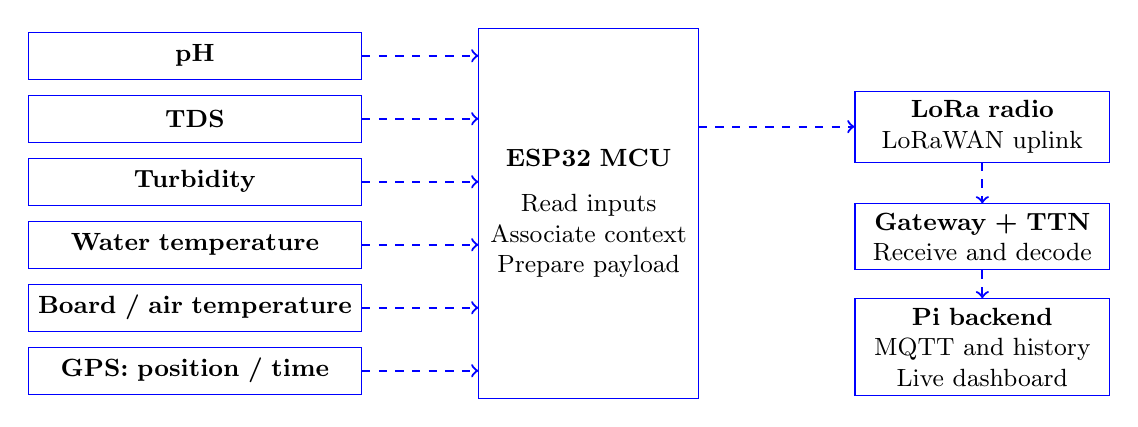
\begin{tikzpicture}[every node/.style={align=center,font=\small},input/.style={draw=blue,text width=4cm,minimum height=.6cm},output/.style={draw=blue,text width=3cm,minimum height=.8cm}]
\node[input] (ph) at (0,0) {\textbf{pH}};
\node[input] (tds) at (0,-.8) {\textbf{TDS}};
\node[input] (turbidity) at (0,-1.6) {\textbf{Turbidity}};
\node[input] (water) at (0,-2.4) {\textbf{Water temperature}};
\node[input] (board) at (0,-3.2) {\textbf{Board / air temperature}};
\node[input] (gps) at (0,-4) {\textbf{GPS: position / time}};
\node[draw=blue,inner sep=0,minimum width=2.8cm,minimum height=4.7cm,text width=2.6cm] (mcu) at (5,-2) {\textbf{ESP32 MCU}\\[.6em]Read inputs\\Associate context\\Prepare payload};
\node[output] (radio) at (10,-.9) {\textbf{LoRa radio}\\LoRaWAN uplink};
\node[output] (gateway) at (10,-2.3) {\textbf{Gateway + TTN}\\Receive and decode};
\node[output] (backend) at (10,-3.7) {\textbf{Pi backend}\\MQTT and history\\Live dashboard};
\draw[->,thick,dashed,blue] (ph.east)--(3.6,0);
\draw[->,thick,dashed,blue] (tds.east)--(3.6,-.8);
\draw[->,thick,dashed,blue] (turbidity.east)--(3.6,-1.6);
\draw[->,thick,dashed,blue] (water.east)--(3.6,-2.4);
\draw[->,thick,dashed,blue] (board.east)--(3.6,-3.2);
\draw[->,thick,dashed,blue] (gps.east)--(3.6,-4);
\draw[->,thick,dashed,blue] (6.4,-.9)--(radio.west);
\draw[->,thick,dashed,blue] (radio.south)--(gateway.north);
\draw[->,thick,dashed,blue] (gateway.south)--(backend.north);
\end{tikzpicture}
\end{center}
\begin{itemize}
    \item \textbf{Measurements need context}: location, time and device identity travel with the observations.
    \item \textbf{The dashboard brings them together}; it does not replace the physical sensors.
\end{itemize}
\vfill{\scriptsize Functional data connections, not pin assignments. Sensor inputs include analog channels and digital interfaces.}
\end{frame}

% Slide 11
\begin{frame}{Workshop Impressions -- 2024}{Making the Connections: Soldering and Inspection}
\centering
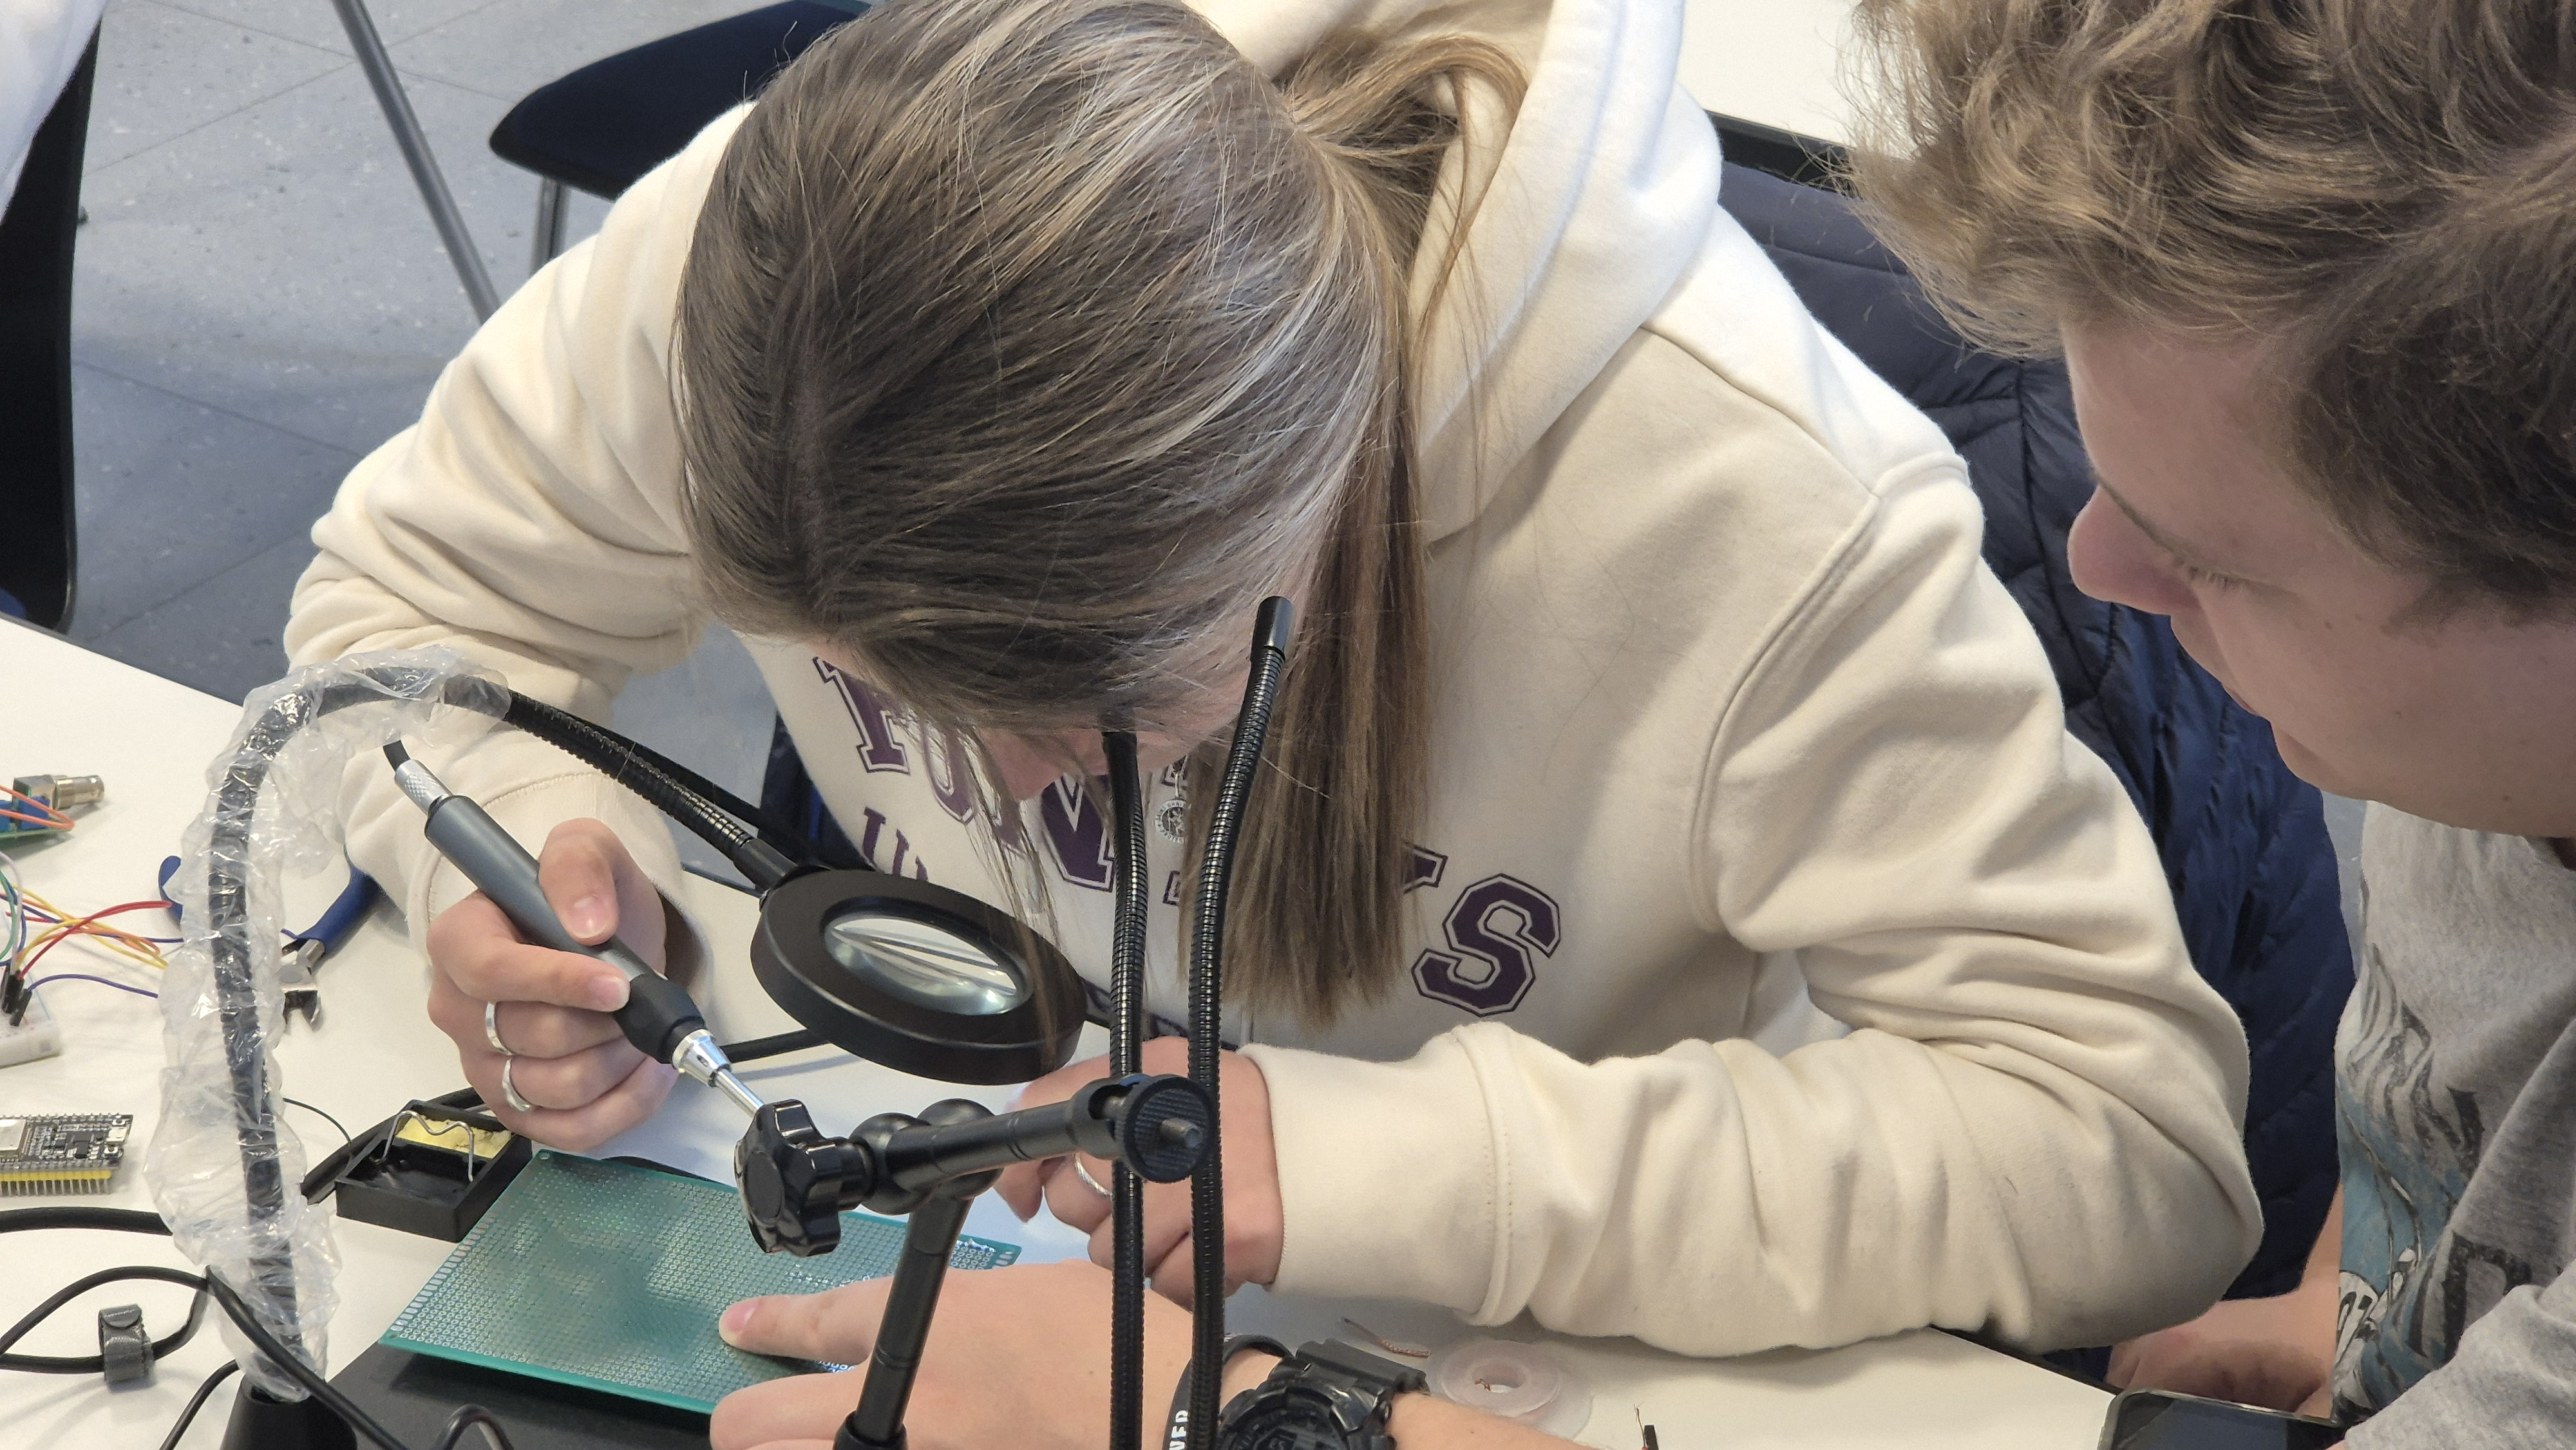
\includegraphics[width=\textwidth,height=.70\paperheight,keepaspectratio]{slides/035-ga-in-it-202425/material/20241104_124213.jpg}
\par\smallskip{\small Physical connections \quad$\cdot$\quad Careful assembly \quad$\cdot$\quad Checking the result}
\end{frame}

% Slide 12
\begin{frame}{Workshop Impressions -- 2024}{Wiring, Checking and Learning Together}
\centering
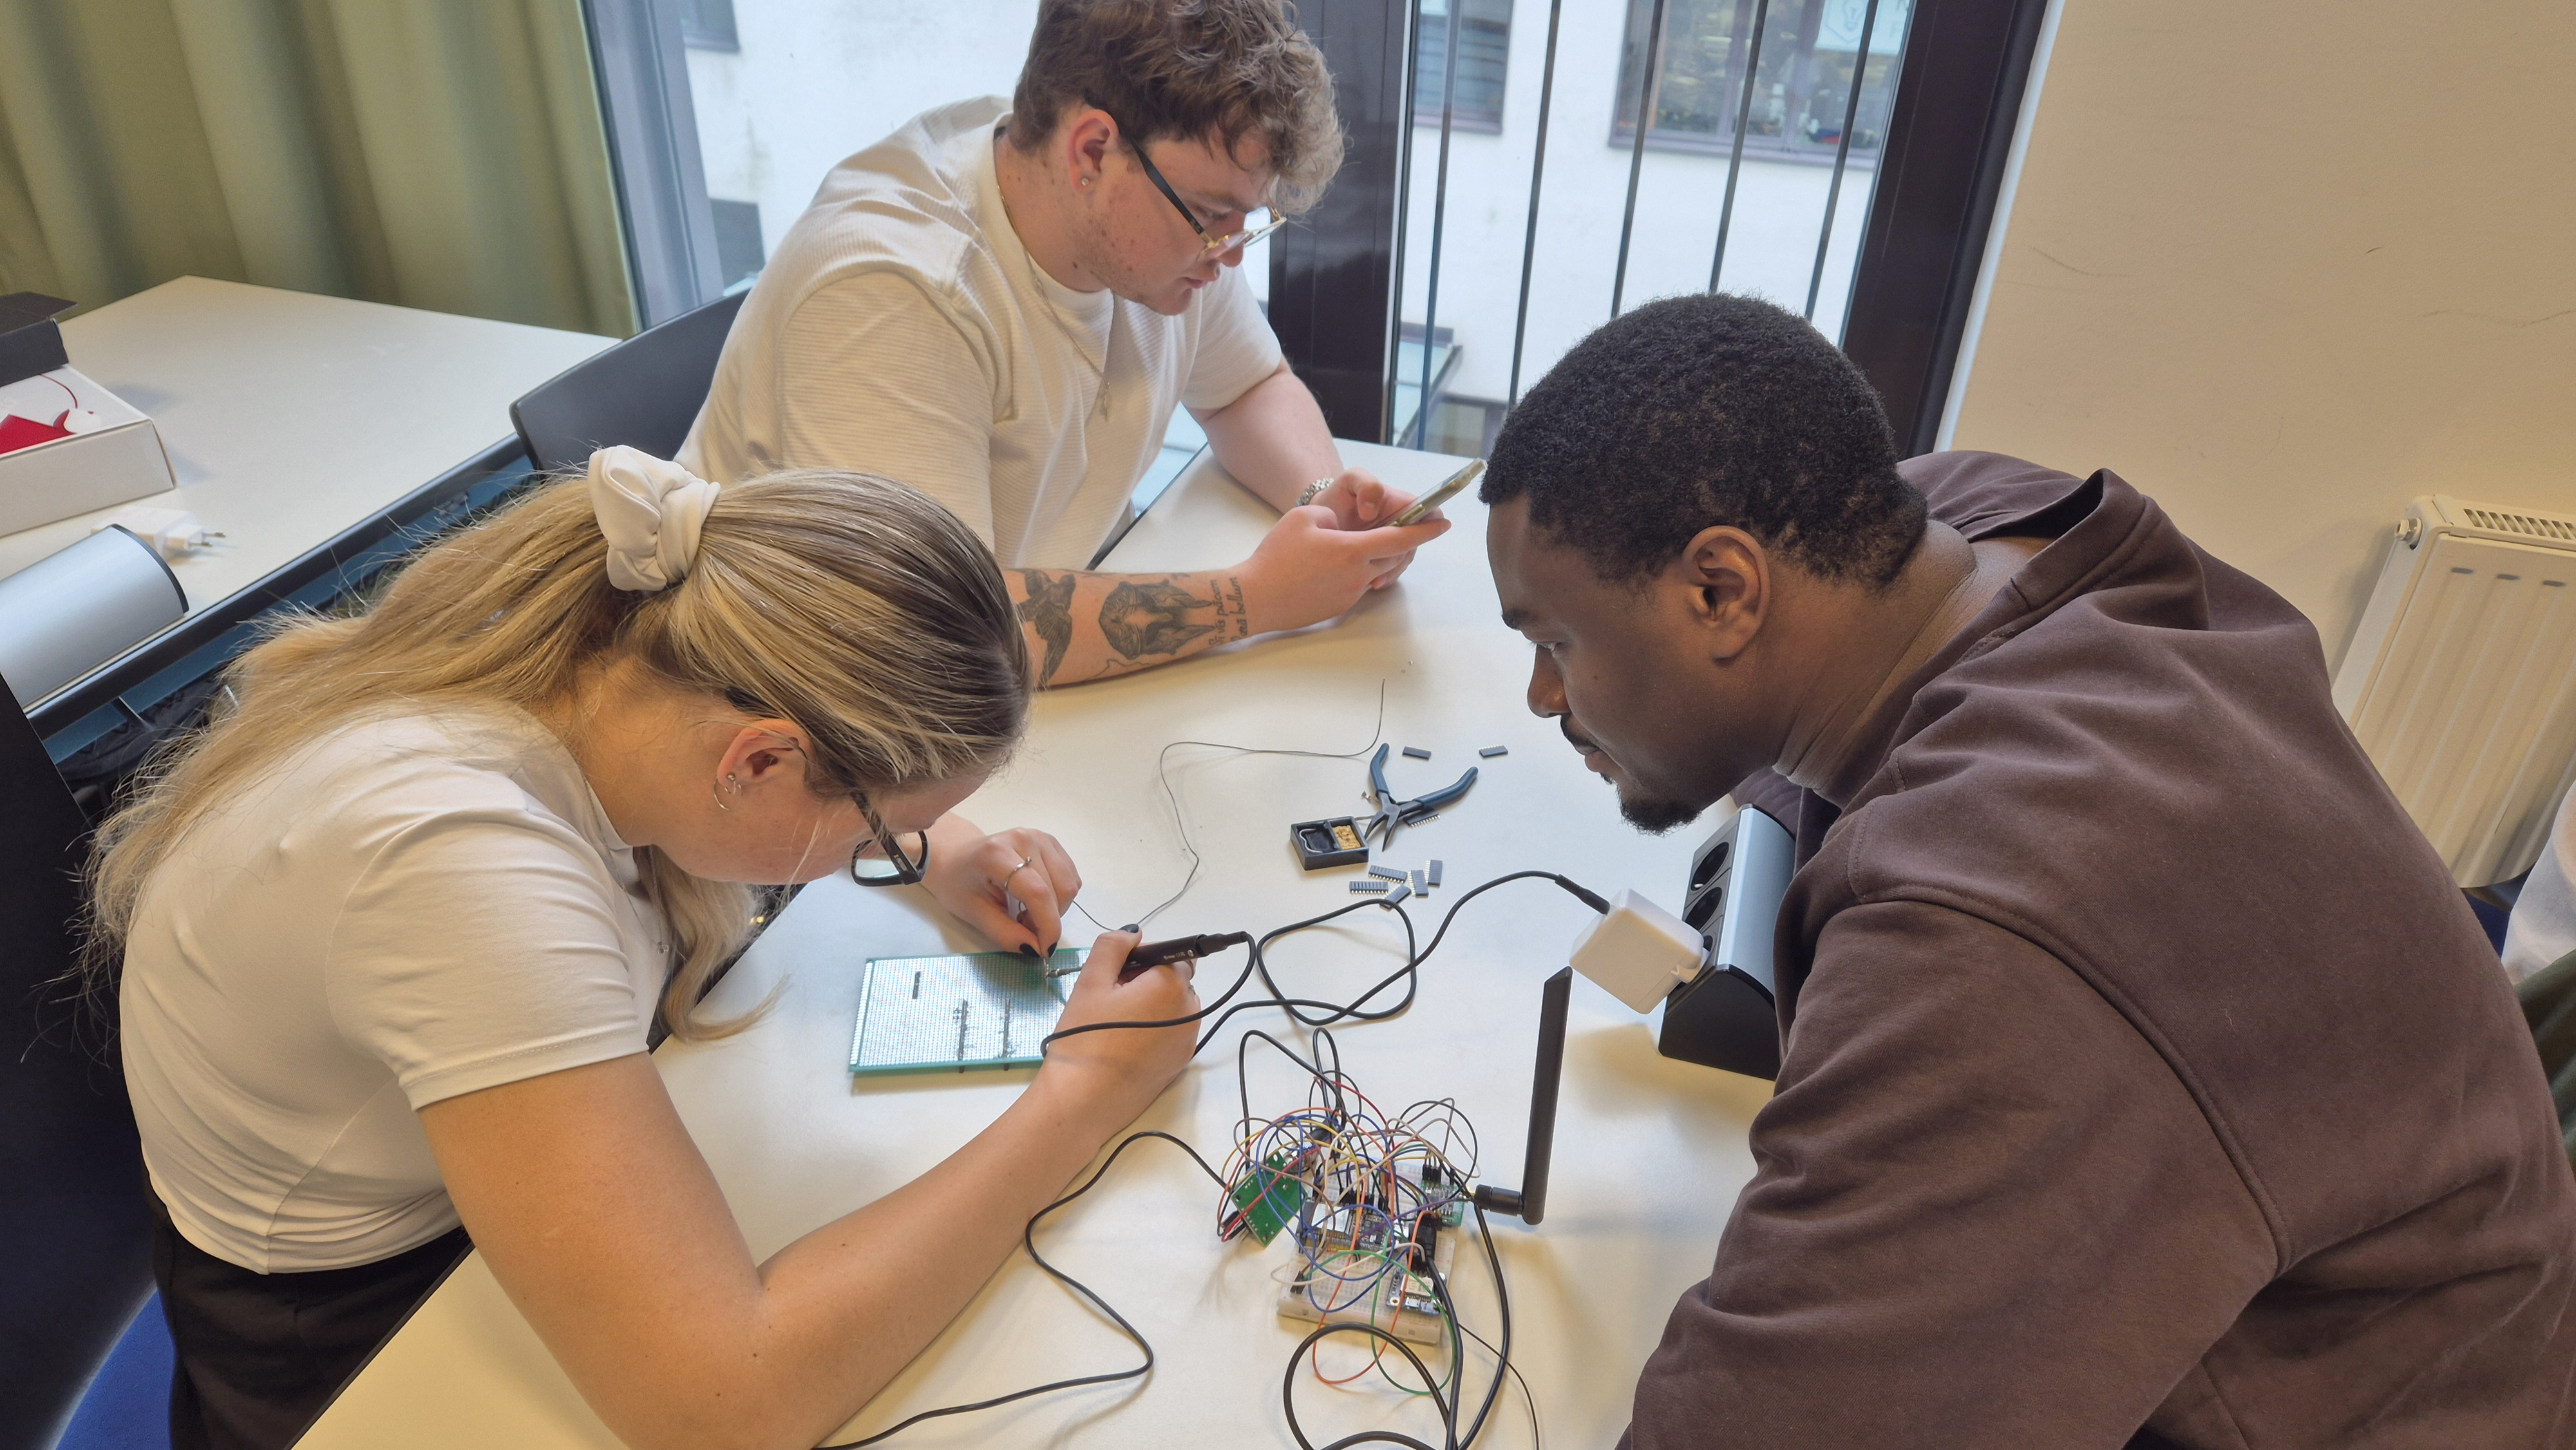
\includegraphics[width=\textwidth,height=.70\paperheight,keepaspectratio]{slides/035-ga-in-it-202425/material/20241105_102406.jpg}
\par\smallskip{\small Shared reasoning \quad$\cdot$\quad Sensor connections \quad$\cdot$\quad Integration}
\end{frame}

% Slide 13
\begin{frame}{Inside the Buoy: From Water to Useful Information}{Every Component Serves the Research Question}
\begin{center}
\begin{tikzpicture}[every node/.style={align=center,font=\small,text width=2.15cm}]
\node (a) at (0,0) {\textbf{Water conditions}\\Physical world};
\node (b) at (2.8,0) {\textbf{Sensors}\\Observations};
\node (c) at (5.6,0) {\textbf{Wireless link}\\Send readings};
\node (d) at (8.4,0) {\textbf{Data service}\\Store readings};
\node (e) at (11.2,0) {\textbf{Dashboard}\\Interpret them};
\draw[->,thick,fh-ooe-red] (a)--(b);
\draw[->,thick,fh-ooe-red] (b)--(c);
\draw[->,thick,fh-ooe-red] (c)--(d);
\draw[->,thick,fh-ooe-red] (d)--(e);
\end{tikzpicture}
\end{center}
\vspace{.8em}
\begin{itemize}
    \item \textbf{Sensors translate conditions into readings}: temperature, pH or conductivity are examples.
    \item A microcontroller links each reading to \textbf{when and where it was taken}.
    \item Wireless communication carries information \textbf{from the water to the people investigating it}.
    \item \textbf{Stored observations reveal patterns}; researchers still need to interpret them.
\end{itemize}
\vfill
\alert{The useful result is evidence about the environment, not the sensor itself.}
\end{frame}

% Slide 14
\begin{frame}{The Buoy: From Radio to a Live Dashboard}{Where the Network and Backend Services Run}
\begin{center}
\begin{tikzpicture}[every node/.style={align=center,font=\small},service/.style={draw=fh-ooe-red,text width=2cm,minimum height=.7cm}]
\draw[gray] (7.65,.72) rectangle (13.35,-3.45);
\node[font=\small\bfseries] at (10.5,1) {Raspberry Pi: local backend};
\node[service] (buoy) at (0,0) {Buoy MCU};
\node[service] (gw) at (3,0) {LoRaWAN\\gateway};
\node[service] (ttn) at (6,0) {TTN\\Network service};
\node[service] (mqtt) at (9,0) {MQTT broker};
\node[service] (store) at (12,0) {Storage service};
\node[service] (db) at (12,-1.6) {MariaDB\\History};
\node[service] (dash) at (9,-2.85) {Dashboard server};
\node[service] (browser) at (5.3,-2.85) {Browser\\Live view};
\draw[->,thick,fh-ooe-red] (buoy.east)--(gw.west);
\draw[->,thick,fh-ooe-red] (gw.east)--(ttn.west);
\draw[->,thick,fh-ooe-red] (ttn.east)--(mqtt.west);
\draw[->,thick,fh-ooe-red] (mqtt.east)--(store.west);
\draw[->,thick,fh-ooe-red] (store.south)--(db.north);
\draw[->,thick,blue] (mqtt.south)-- node[left,font=\scriptsize]{Live readings} (dash.north);
\draw[->,thick,fh-ooe-red] (db.south)|-(dash.east);
\node[font=\scriptsize] at (11.2,-2.6) {History};
\draw[->,thick,blue] (dash.west)--node[above]{SSE} (browser.east);
\node[font=\scriptsize,align=left] at (1.2,-1.6) {\textcolor{fh-ooe-red}{Red: uplink / stored history}\\\textcolor{blue}{Blue: live readings / SSE}};
\end{tikzpicture}
\end{center}
\begin{itemize}
    \item \textbf{A bridge brings TTN messages to local MQTT}, which feeds storage and the dashboard.
    \item \textbf{MariaDB retains history}; the browser also receives \textbf{live updates via SSE}.
    \item \textbf{Server-Sent Events} keep the browser current without manual refresh.
\end{itemize}
\vfill{\scriptsize Shared teaching architecture; not a claim that this exact backend was deployed in 2024.}
\end{frame}


% Slide 15
\begin{frame}{One Observation, All the Way to the Researcher}{An Illustrative Temperature Reading -- Not Field Data}
\begin{columns}[c,onlytextwidth]
\column{.57\textwidth}
\begin{enumerate}
    \item \textbf{Sensor and MCU}: record 24.0\,$^\circ$C, with time, location and device identity.
    \item \textbf{LoRaWAN and TTN}: carry and decode the observation; MQTT brings it to the Pi.
    \item \textbf{Storage and MariaDB}: preserve the reading for later comparison.
    \item \textbf{Dashboard and SSE}: show the new reading alongside earlier observations.
\end{enumerate}
\column{.39\textwidth}
\begin{tikzpicture}[every node/.style={align=center}]
\node[draw=fh-ooe-red,inner sep=12pt] (reading) at (0,1.1) {\textbf{Illustrative reading}\\[.6em]{\Huge 24.0\,$^\circ$C}\\[.6em]Water temperature};
\node[text width=4.5cm] (question) at (0,-1.55) {\textbf{Research question}\\How does this location compare with earlier observations or other locations?};
\draw[->,thick,fh-ooe-red] (reading)--(question);
\end{tikzpicture}
\end{columns}
\vfill\alert{One reading is a starting point. Context and repeated observations make it useful.}
\end{frame}

% Slide 16
\begin{frame}{2025: The Challenge Continues}{The Same Invasive-Species Theme -- Another Cohort's Contribution}
\begin{columns}[c,onlytextwidth]
\column{.51\textwidth}
\begin{itemize}
    \item \textbf{The same research challenge} continues with a new cohort.
    \item \textbf{Sensor nodes and LoRaWAN} connect water observations to the network.
    \item \textbf{Data services and storage} make readings available beyond the device.
    \item A \textbf{web interface} brings measurements and locations together for interpretation.
\end{itemize}
\column{.45\textwidth}
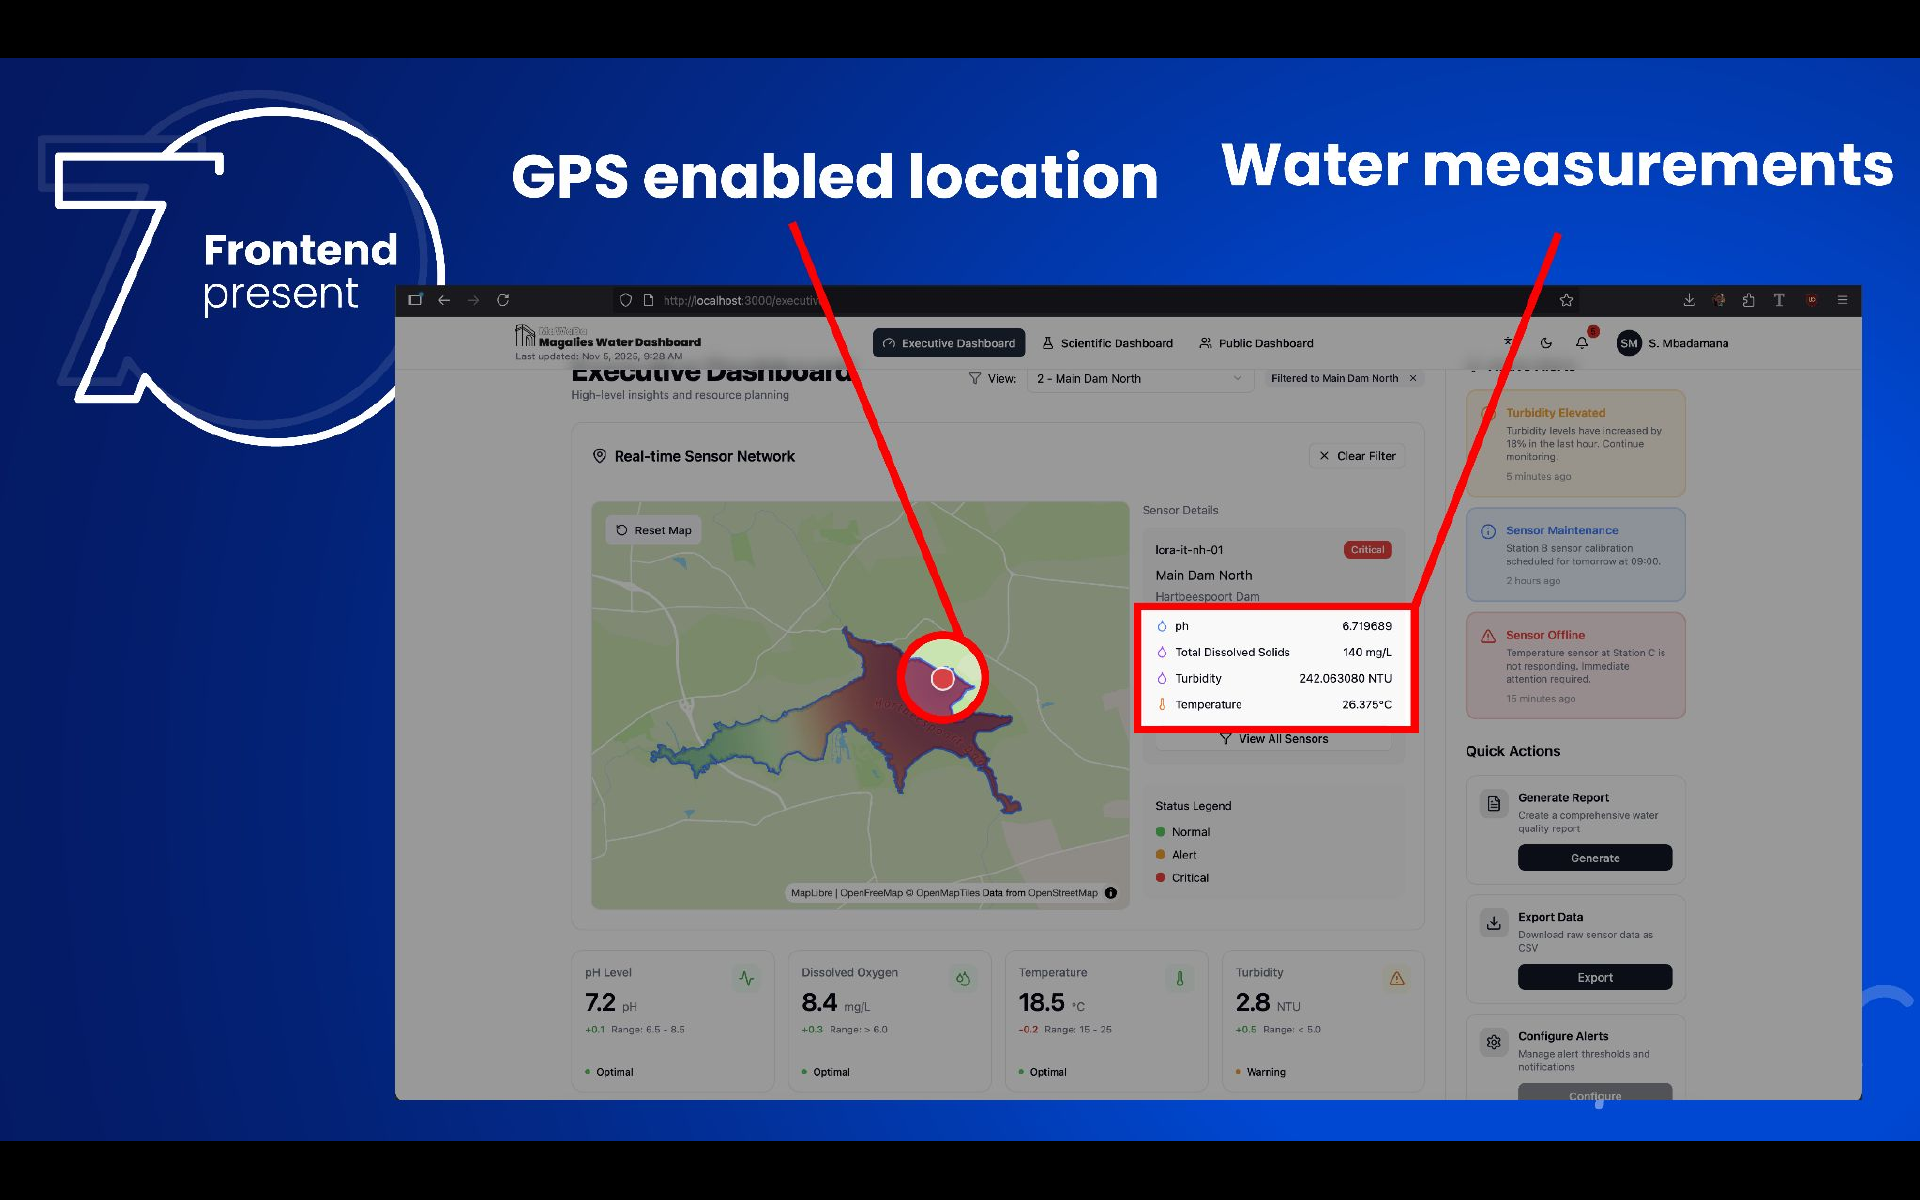
\includegraphics[width=\linewidth,height=.57\paperheight,keepaspectratio]{slides/035-ga-in-it-202425/material/Screenshot_20260124_194420.png}
\par\smallskip{\scriptsize Monitoring implementation shown in the 2025 project material.}
\end{columns}
\end{frame}

% Slide 17
\begin{frame}{When Does Monitoring Become Useful?}{A Working Prototype Is One Step in a Longer Chain}
\begin{itemize}
    \item \textbf{Trustworthy measurements}: calibration, coverage and missing data matter.
    \item \textbf{Someone can use them}: researchers need access, context and time to interpret them.
    \item \textbf{A decision can follow}: information must connect to a practical choice or investigation.
    \item \textbf{Benefits need evidence}: collecting data does not itself demonstrate ecosystem recovery.
\end{itemize}
\vspace{.8em}
\begin{center}
{\large Measurements $\longrightarrow$ Understanding $\longrightarrow$ Decisions $\longrightarrow$ Action}
\end{center}
\vspace{.4em}
\alert{Who takes the next step after the dashboard?}
\end{frame}

\part[nopartpage]{2026 -- Understanding Green Energy}
% Slide 18
\begin{frame}{2026: A New Theme -- Green Energy}{A Different Challenge, the Same Starting Point}
\begin{center}
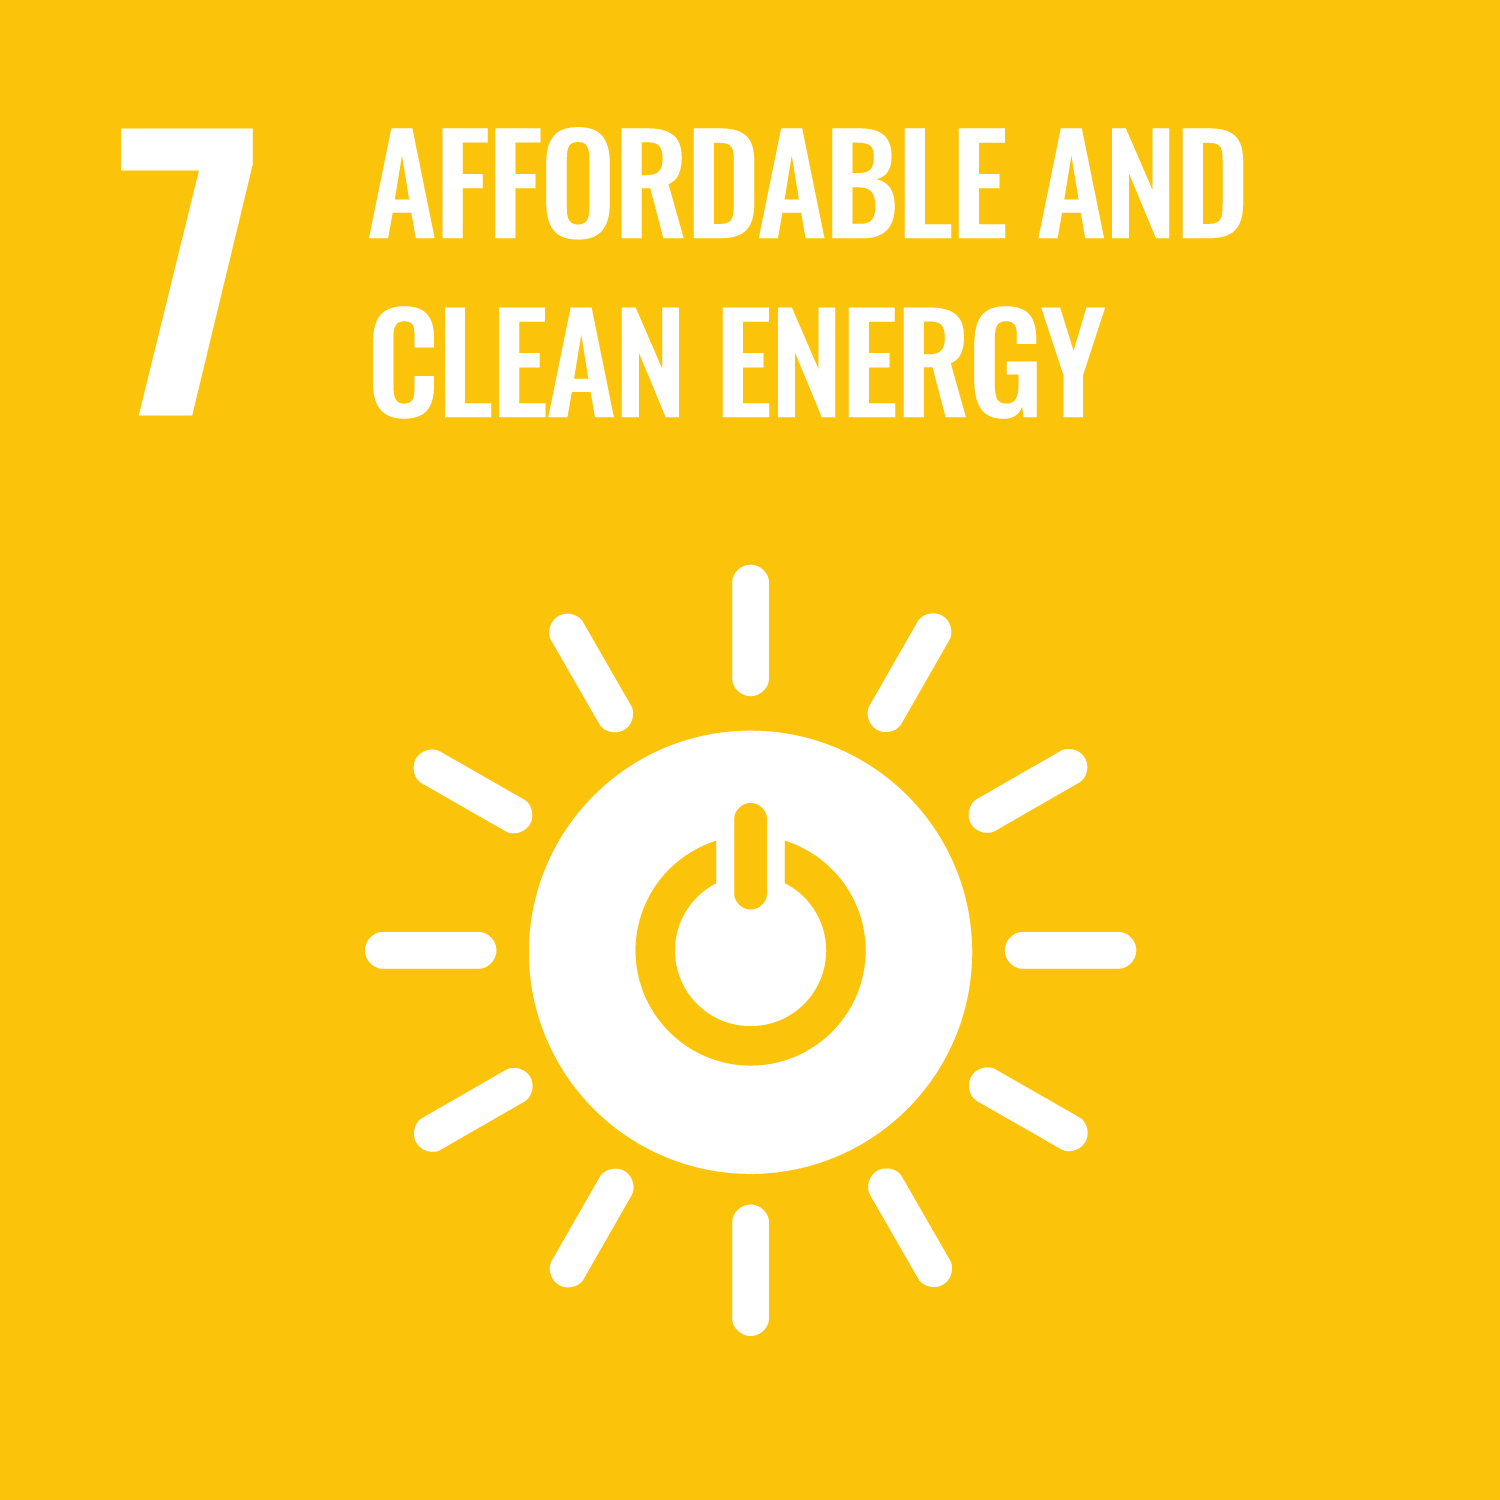
\includegraphics[height=.9cm]{slides/036-sdg-story/material/sdg-icons/goal-07.png}\hspace{.6em}

\includegraphics[height=.9cm]{slides/036-sdg-story/material/sdg-icons/goal-04.png}
\end{center}
\begin{itemize}
    \item \textbf{Generation, storage and consumption} have to work together.
    \item Energy availability changes; \textbf{people must make choices} about when and how to use it.
    \item A useful project should help a community \textbf{understand or manage those choices}.
    \item Start with the purpose; leave room for \textbf{students to shape the response}.
\end{itemize}
\vspace{.6em}
\begin{center}
{\large Sun $\longrightarrow$ Generation $\longleftrightarrow$ Storage $\longrightarrow$ Use}
\end{center}
\vfill
{\footnotesize \textbf{SDG connection:} renewable energy (7.2) and learning for sustainable development (4.7).\par}
{\scriptsize UN targets: \href{https://sdgs.un.org/goals/goal7}{Goal 7} / \href{https://sdgs.un.org/goals/goal4}{Goal 4}.}
\end{frame}

% Slide 19
\begin{frame}{Four Ideas to Start the Conversation}{Possible Directions Within One Green-Energy Theme}
\begin{columns}[T,onlytextwidth]
\column{.235\textwidth}\centering
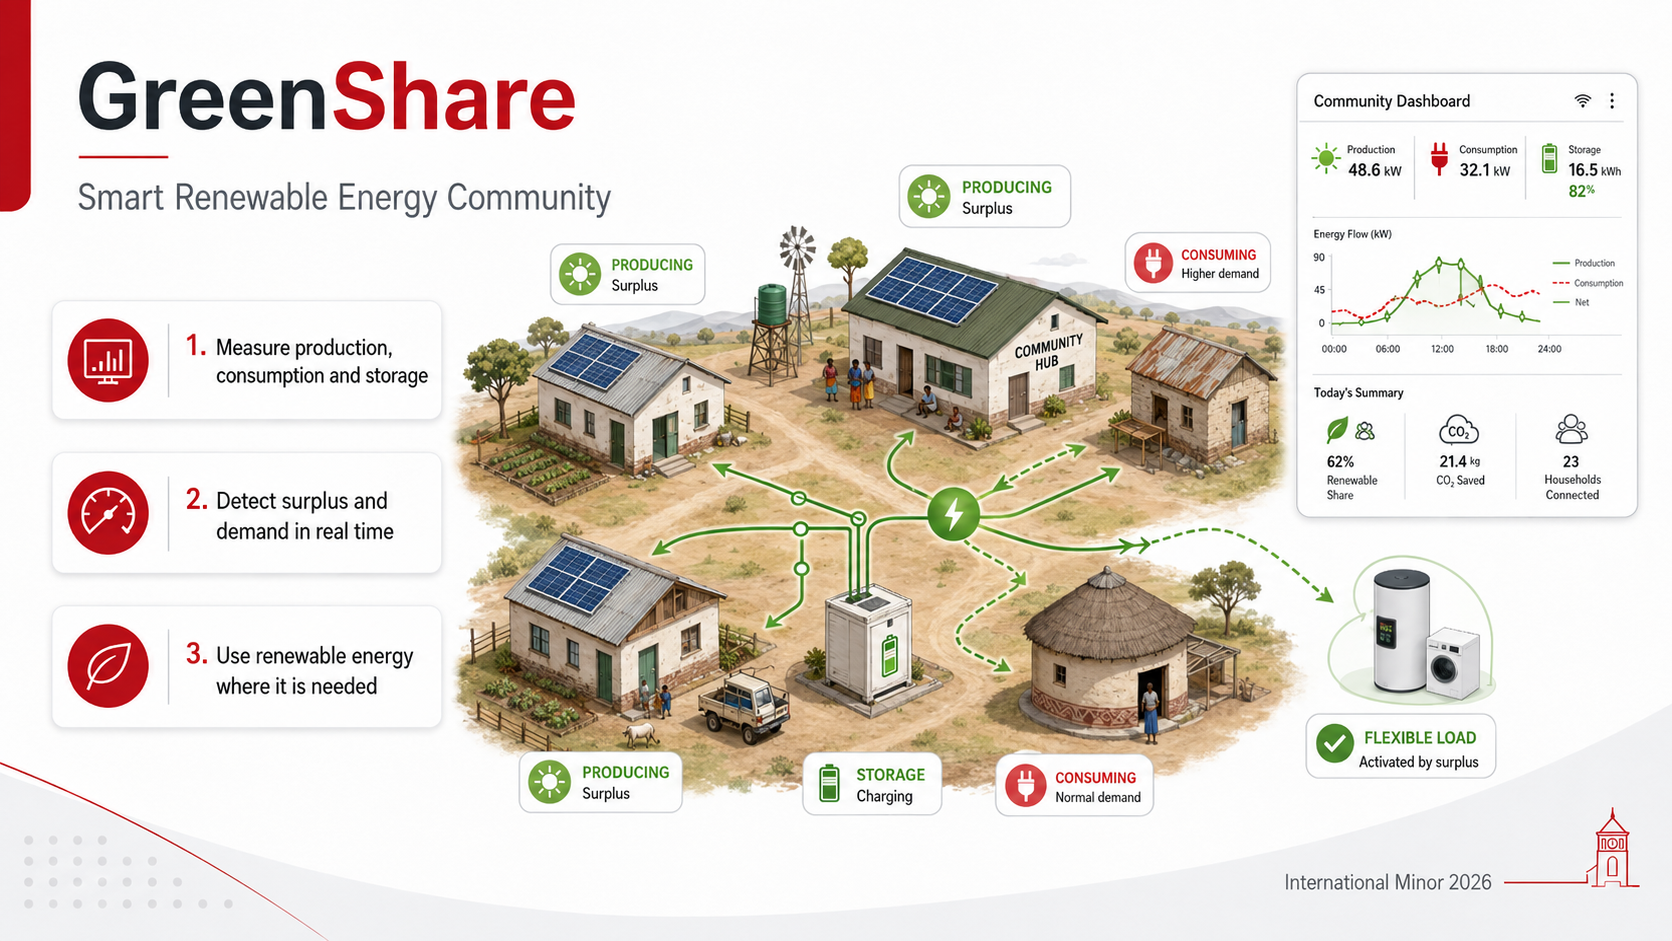
\includegraphics[width=\linewidth]{slides/035-ga-in-it-preintro/material/project-graphics/set-2/greenshare_renewable_energy_community.png}
\par\smallskip\textbf{GreenShare}\par\smallskip Share renewable energy within a community.
\column{.235\textwidth}\centering
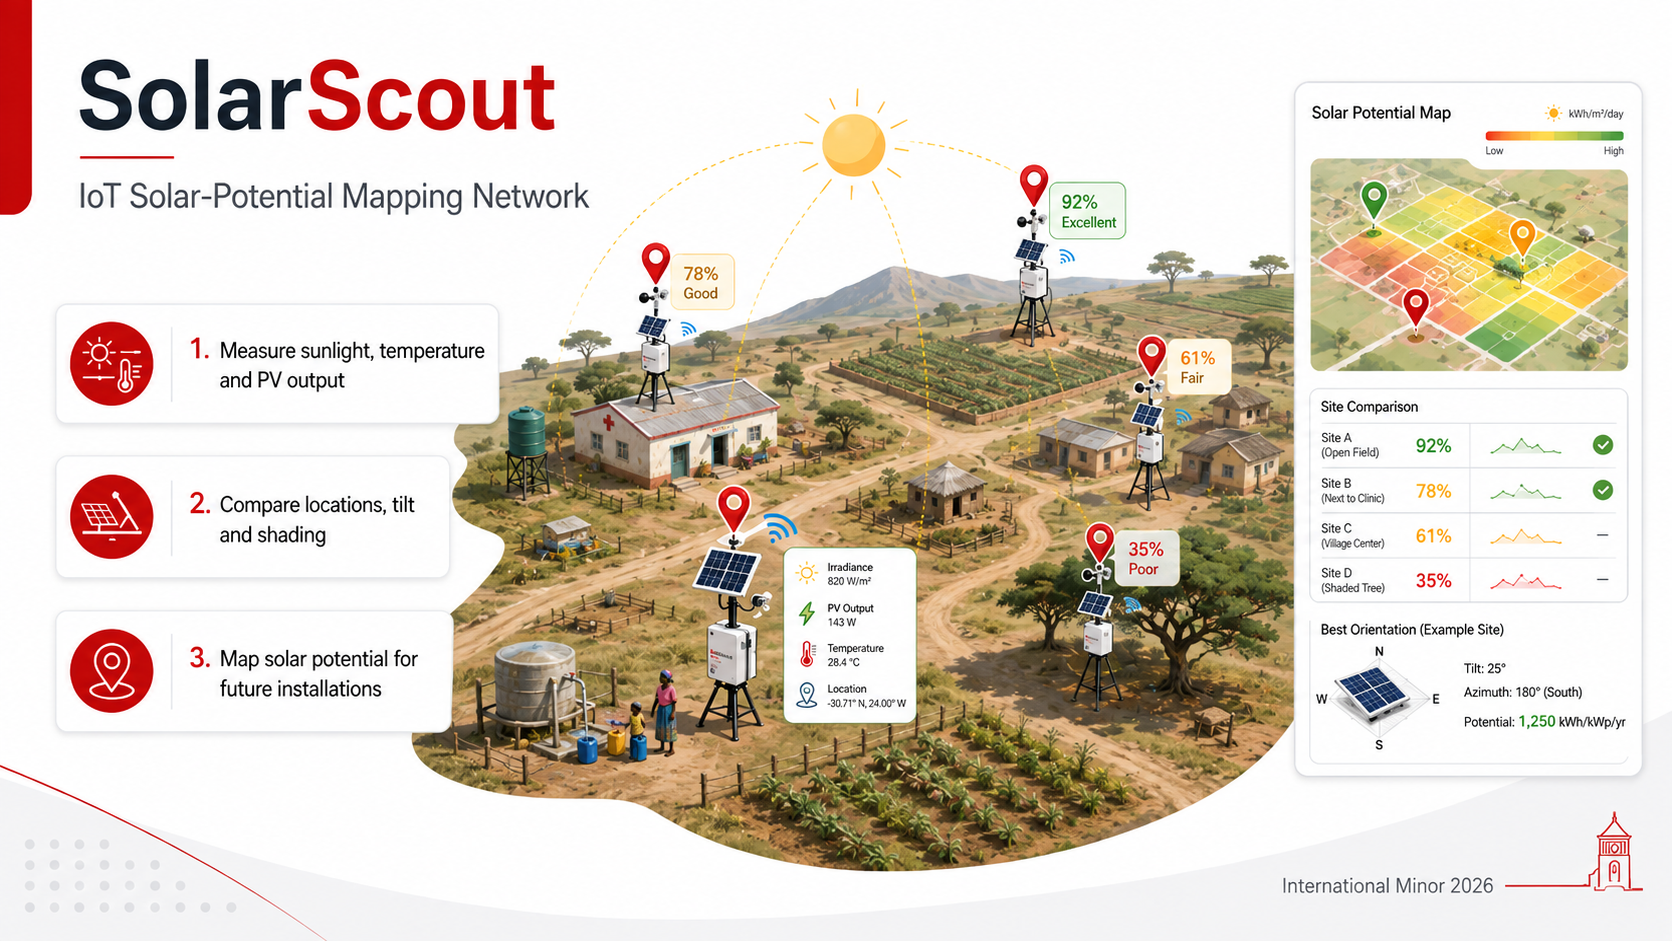
\includegraphics[width=\linewidth]{slides/035-ga-in-it-preintro/material/project-graphics/set-2/solarscout_mapping_solar_potential.png}
\par\smallskip\textbf{SolarScout}\par\smallskip Explore where solar generation could work.
\column{.235\textwidth}\centering
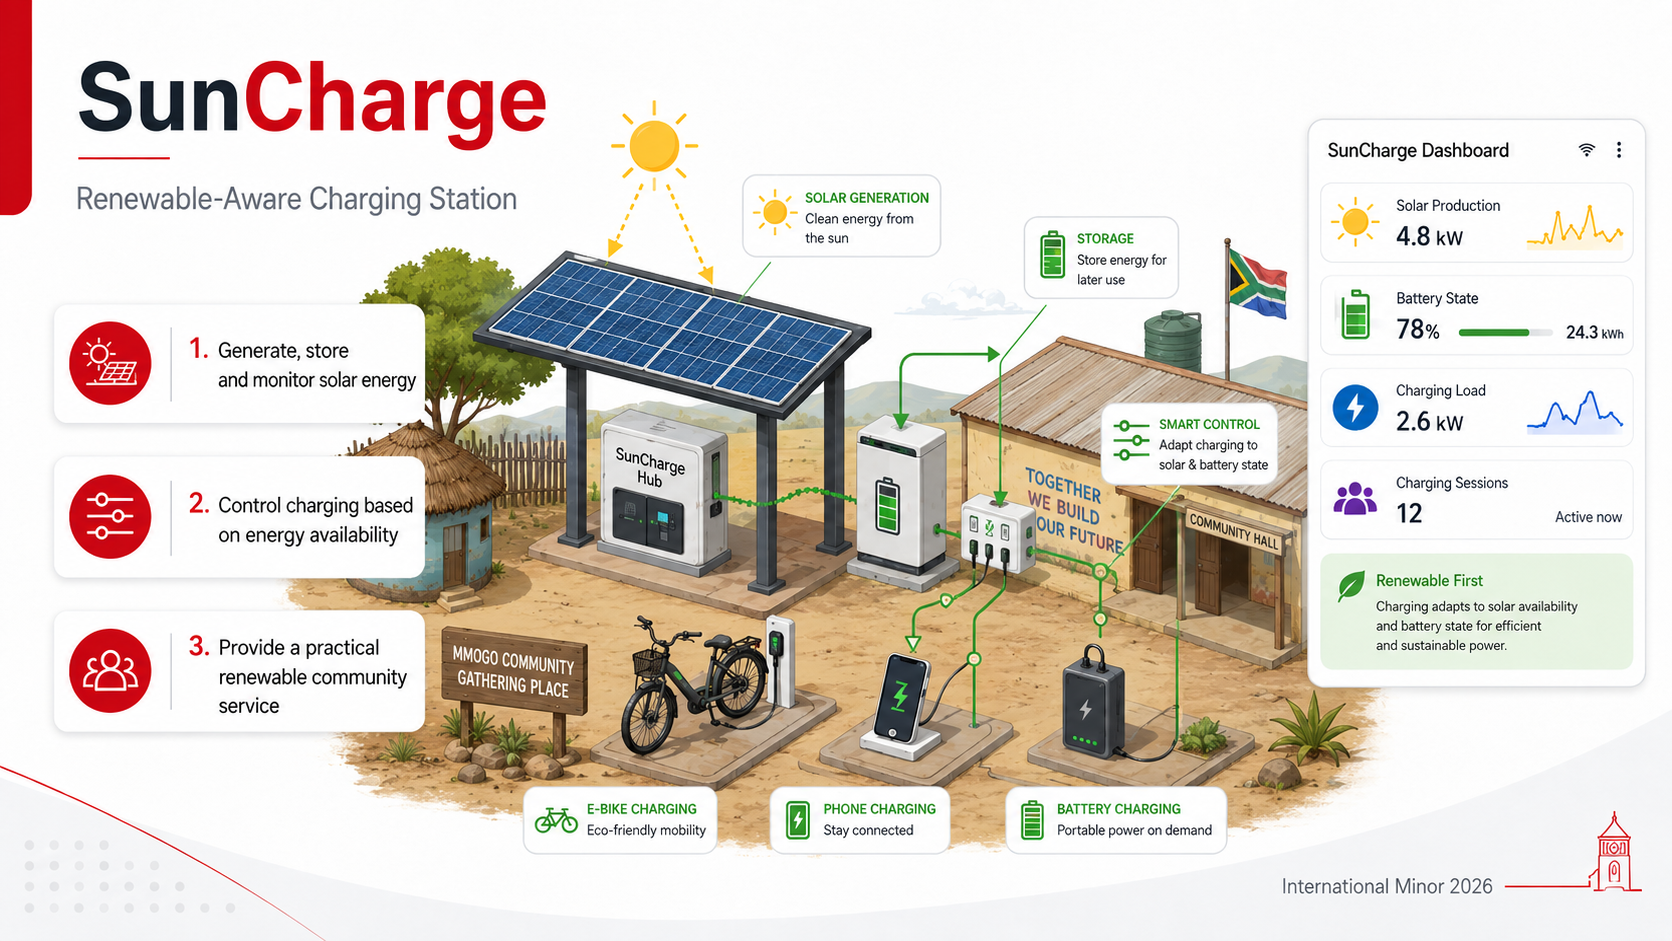
\includegraphics[width=\linewidth]{slides/035-ga-in-it-preintro/material/project-graphics/set-2/suncharge_community_renewable_charging_hub.png}
\par\smallskip\textbf{SunCharge}\par\smallskip Charge devices when renewable energy is available.
\column{.235\textwidth}\centering
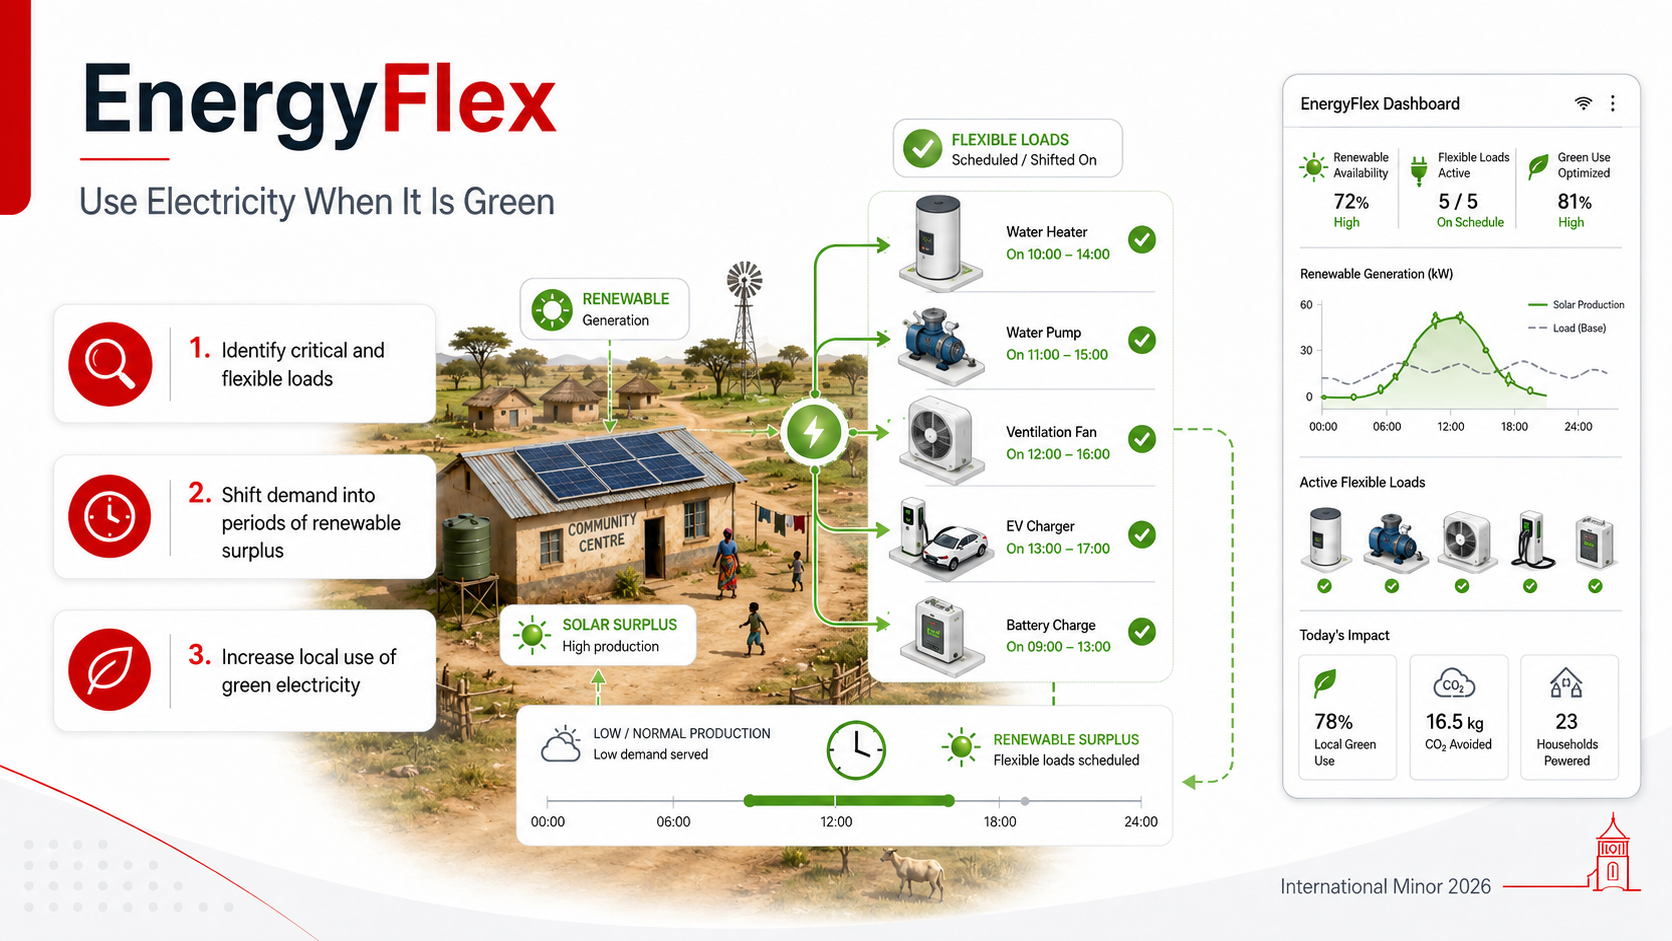
\includegraphics[width=\linewidth]{slides/035-ga-in-it-preintro/material/project-graphics/set-2/energyflex_renewable_village_dashboard.png}
\par\smallskip\textbf{EnergyFlex}\par\smallskip Coordinate demand with energy availability.
\end{columns}
\vspace{1em}
\alert{These were starting points for discussion. The shared project could evolve.}
\vfill{\scriptsize Concept graphics from the existing project proposals; not photographs of built systems.}
\end{frame}

% Slide 20
\begin{frame}{The Students Bring a Gamified Learning Idea}{Start with People Who Are New to Electricity}
\begin{itemize}
    \item The intended learners have \textbf{little or no prior knowledge of electricity}.
    \item Students bring a \textbf{gamified learning idea} and plans for physical gift packages.
    \item Begin with basic questions: \textbf{where does electricity come from, and how can it be stored?}
    \item Could a physical device make these ideas \textbf{understandable through exploration and feedback}?
\end{itemize}
\vspace{.8em}
\begin{center}
{\Large Try an action $\longrightarrow$ Observe a change $\longrightarrow$ Understand}
\end{center}
\end{frame}

% Slide 21
\begin{frame}{Could We Make Those Energy Choices Tangible?}{A Gamified Microgrid Learning Device Takes Shape}
\begin{columns}[c,onlytextwidth]
\column{.53\textwidth}
\begin{itemize}
    \item Bring \textbf{solar generation, storage and consumers} into a small physical system.
    \item Make energy flows and responses \textbf{visible through measurements and a dashboard}.
    \item Use \textbf{challenges and feedback to support learning}; students shape the activities.
    \item Assess \textbf{what learners understand}, alongside what the hardware can do.
\end{itemize}
\column{.43\textwidth}
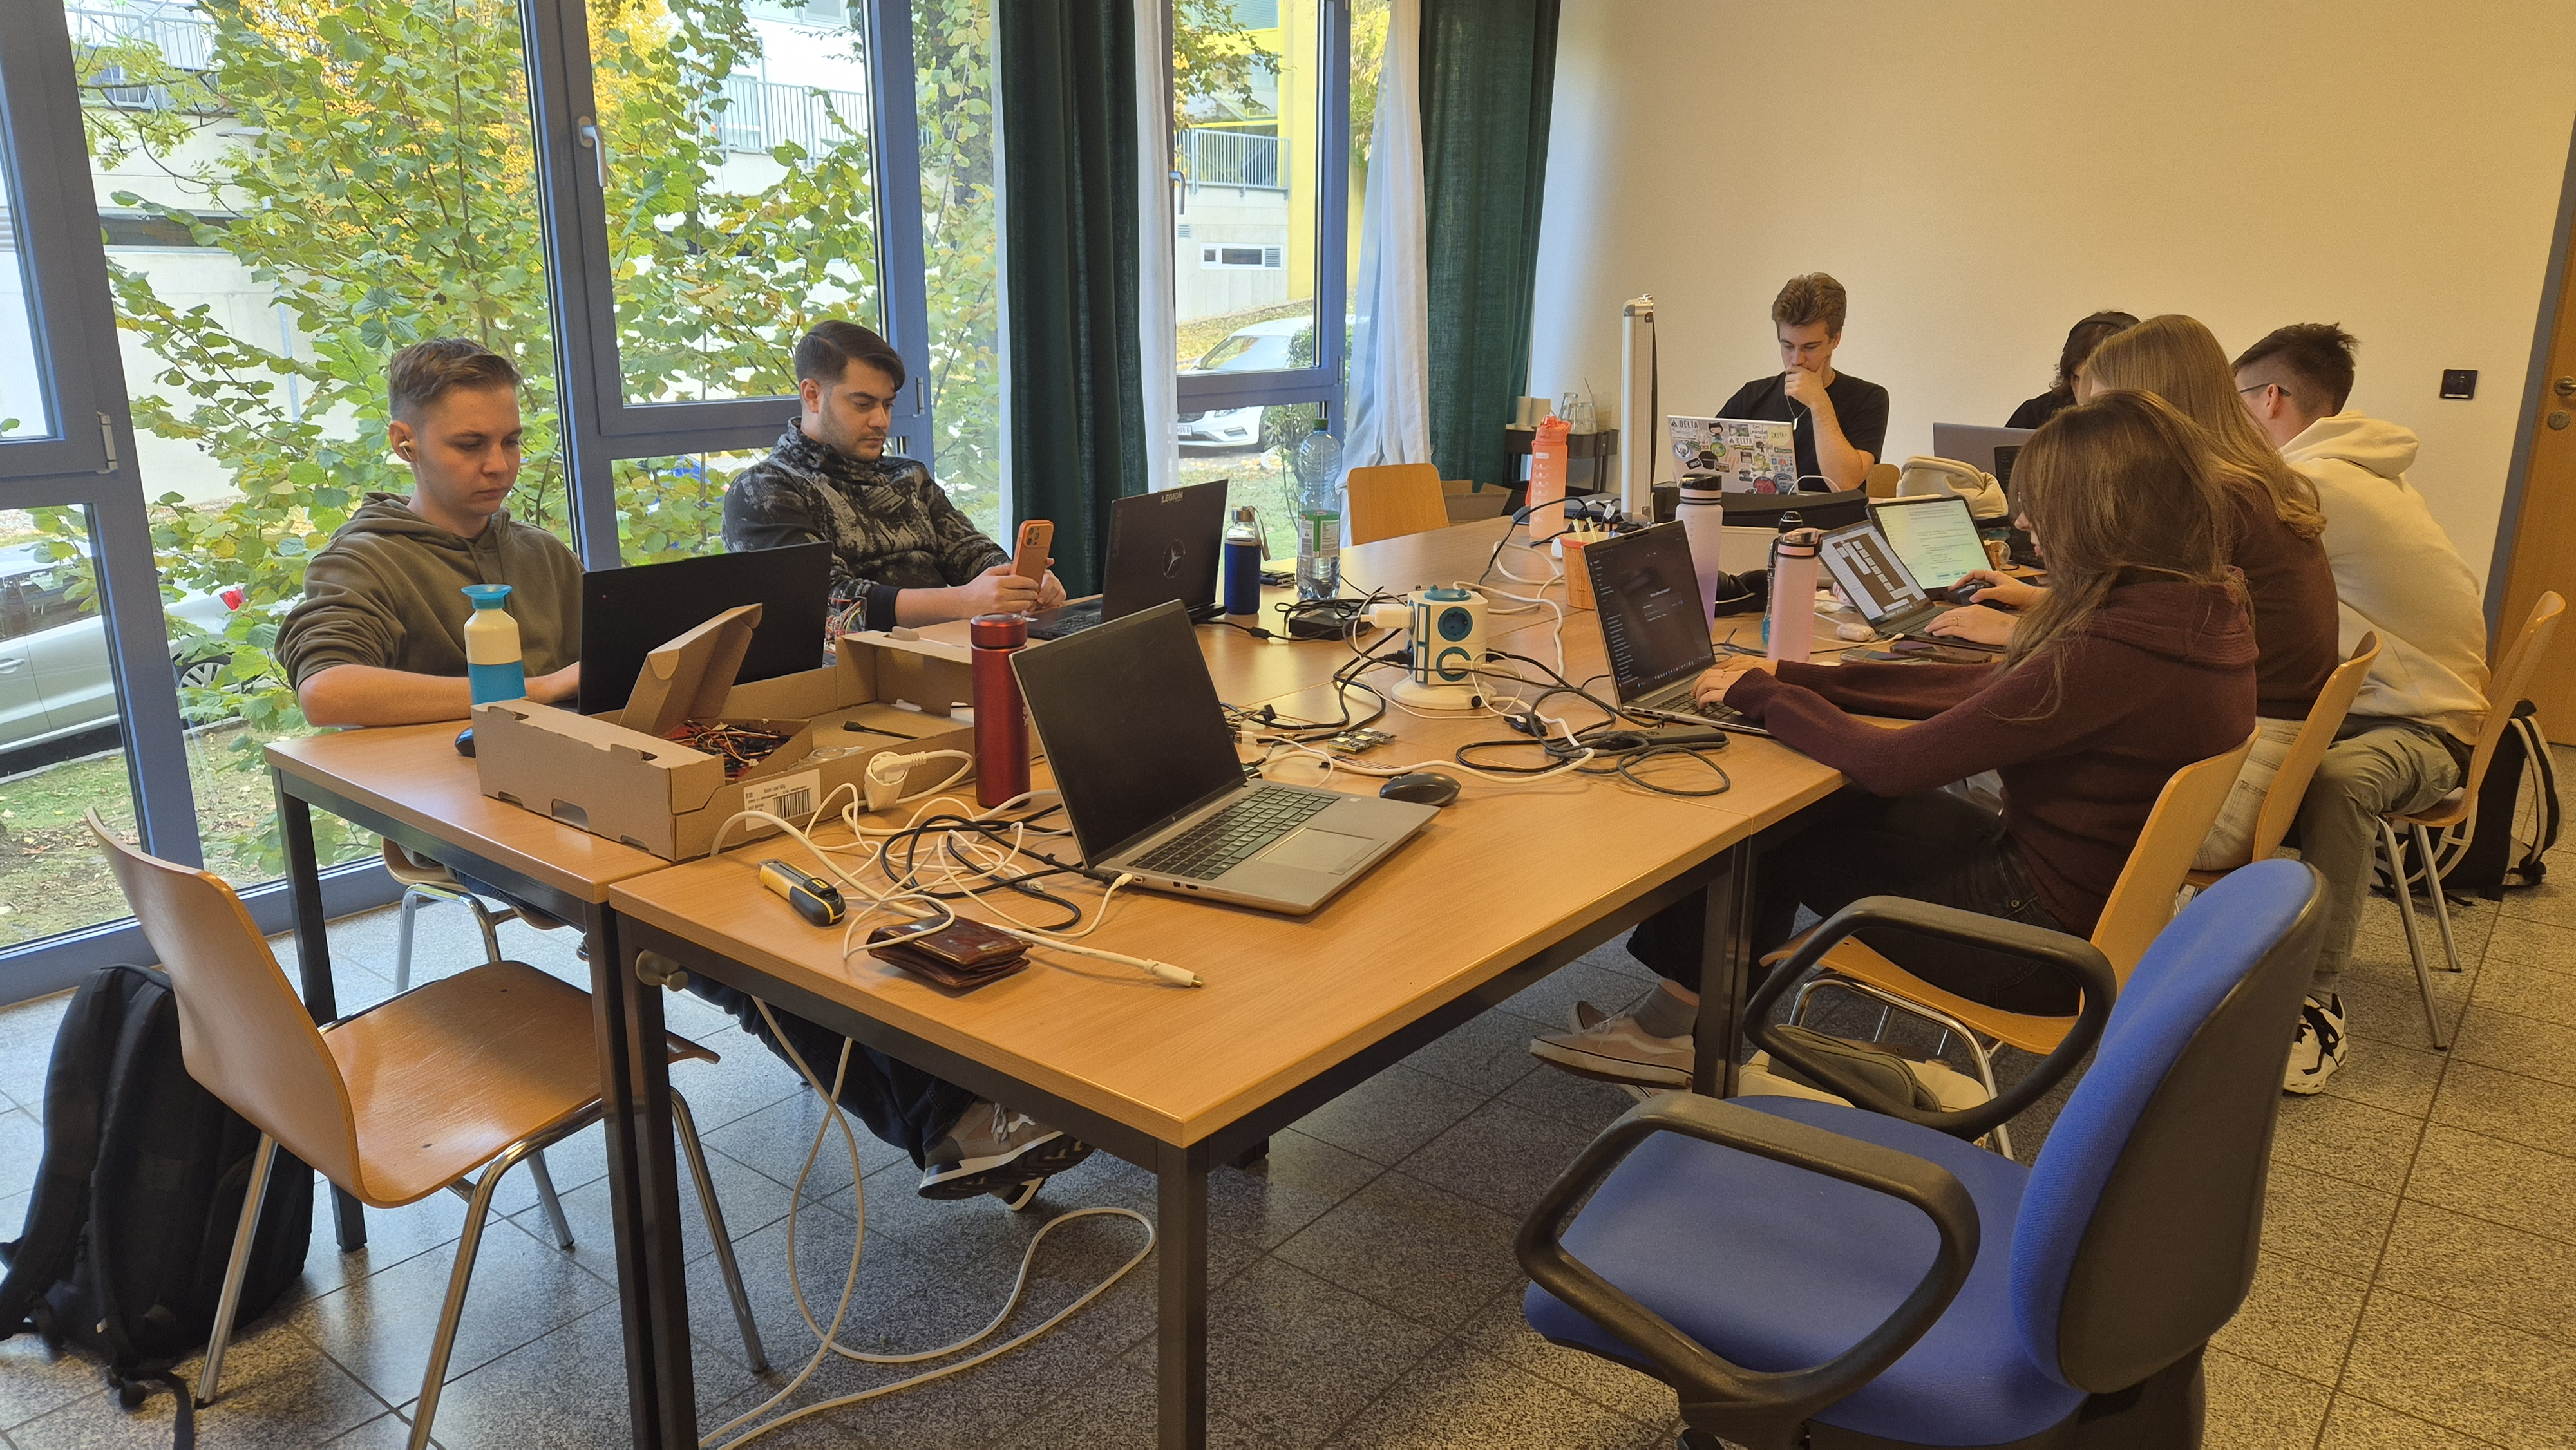
\includegraphics[width=\linewidth,height=.59\paperheight,keepaspectratio]{slides/035-ga-in-it-preintro/material/workshop-impressions-2026/20261030_111806.jpg}
\par\smallskip{\scriptsize The 2026 team developing the shared project.}
\end{columns}
\vfill
{\footnotesize \textbf{SDG 4.7:} learning for sustainable development, using \textbf{SDG 7} as the subject.}
\end{frame}

% Slide 22
\begin{frame}{The Learning Device: Essential Devices}{What Is Visible -- and What Works Inside}
\begin{columns}[c,onlytextwidth]
\column{.51\textwidth}\centering
\begin{tikzpicture}
\node[anchor=south west,inner sep=0] (photo) at (0,0) {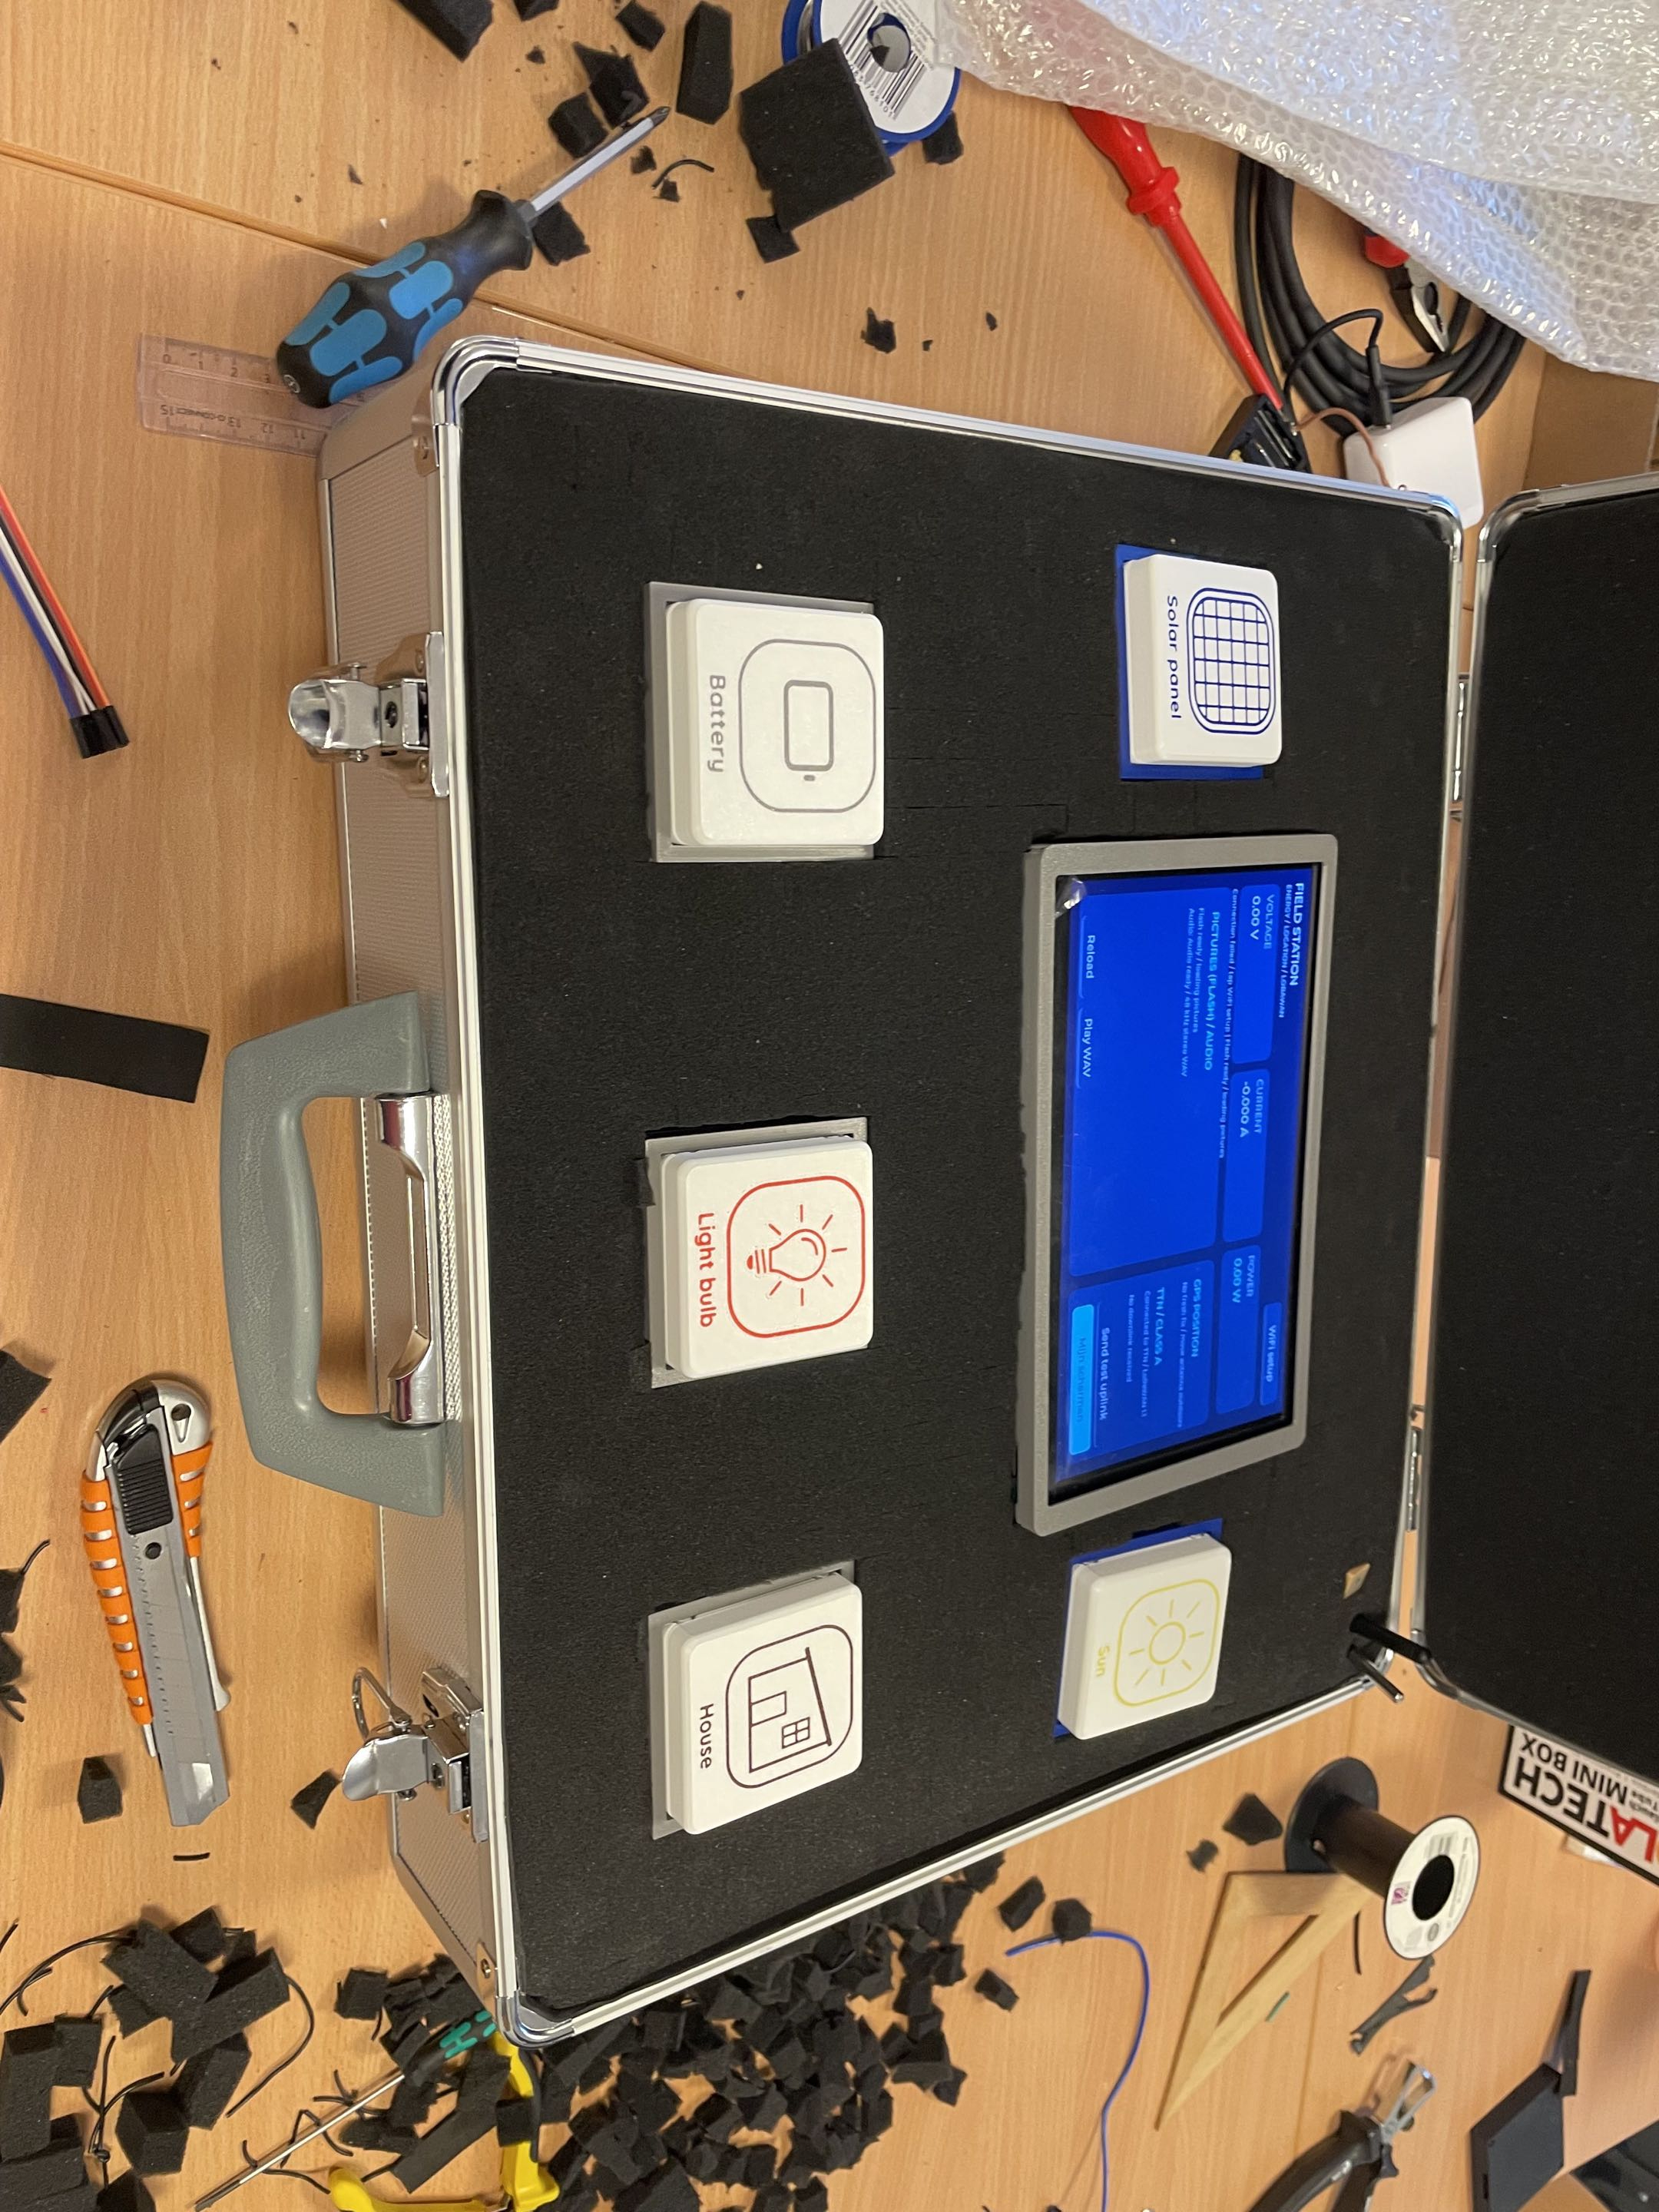
\includegraphics[angle=90,width=\linewidth]{slides/035-ga-in-it-preintro/material/workshop-impressions-2026/image04.jpg}};
\begin{scope}[x={(photo.south east)},y={(photo.north west)}]
\node[circle,fill=fh-ooe-red,text=white,font=\bfseries\small,inner sep=2pt] at (.60,.69) {1};
\node[circle,fill=fh-ooe-red,text=white,font=\bfseries\small,inner sep=2pt] at (.35,.37) {2};
\node[circle,fill=fh-ooe-red,text=white,font=\bfseries\small,inner sep=2pt] at (.50,.19) {3};
\end{scope}
\end{tikzpicture}
\par\smallskip{\small 1 Display \quad 2 Learning elements \quad 3 Case}
\column{.45\textwidth}
\begin{itemize}
    \item \textbf{RFID, temperature, GPS and energy sensors} provide interactions and measurements.
    \item \textbf{The local display, consumers and switches} provide visible information and responses.
    \item \textbf{Raspberry Pi and MQTT} receive suitcase telemetry from TTN and provide the browser dashboard.
\end{itemize}
\vspace{.6em}
{\small\textbf{Components inside: functional view}}\par\smallskip
\begin{tikzpicture}[every node/.style={align=center,font=\small,text width=1.6cm}]
\node (sensors) at (0,0) {Sensors};
\node (mcu) at (2.2,0) {MCU};
\node (pi) at (4.4,0) {LoRa radio};
\draw[->,thick,fh-ooe-red] (sensors)--(mcu);
\draw[->,thick,fh-ooe-red] (mcu)--(pi);
\end{tikzpicture}
\par\smallskip{\scriptsize To gateway, TTN and the Pi backend.}
\end{columns}
\vfill{\scriptsize Photograph: assembled 2026 device. The schematic explains component roles that are hidden in the photograph.}
\end{frame}



% Slide 23
\begin{frame}{The Learning Device: More Than Energy Measurement}{Every Component Has an Educational or Operational Role}
\small\renewcommand{\arraystretch}{1.4}
\par\noindent\begin{tabularx}{\textwidth}{@{}>{\raggedright\arraybackslash}p{.31\textwidth}>{\raggedright\arraybackslash}X@{}}
\toprule
\textbf{Component} & \textbf{Purpose}\\\midrule
\textbf{RFID readers and tags} & Identify learning elements and turn physical interaction into an event the MCU can interpret.\\
\textbf{Temperature sensor} & Adds a temperature observation to the device's measurements.\\
\textbf{GPS receiver} & Supplies position and time when valid information is available.\\
\textbf{Voltage/current sensors} & Observe generation, battery charging/discharging and consumer demand.\\
\textbf{Local display} & Gives explanations, measurements and feedback directly on the device.\\
\textbf{Consumers and switches} & Make energy use and the effects of control visible.\\
\textbf{LoRa radio, gateway and TTN} & Carry the suitcase's observations over LoRaWAN to TTN; TTN's MQTT integration supplies the Pi backend.\\
\textbf{MCU(s), Pi and router} & MCUs manage the device; the Pi hosts MQTT, MariaDB and the dashboard, with network access to TTN.\\\bottomrule
\end{tabularx}\par
\vspace{.5em}
\normalsize\alert{The local display and the browser dashboard are distinct ways to provide feedback.}
\end{frame}

% Slide 24
\begin{frame}{The Learning Device: Complete Peripheral Connections}{Inputs, Local Feedback, Control and Networked Information}
\begin{center}
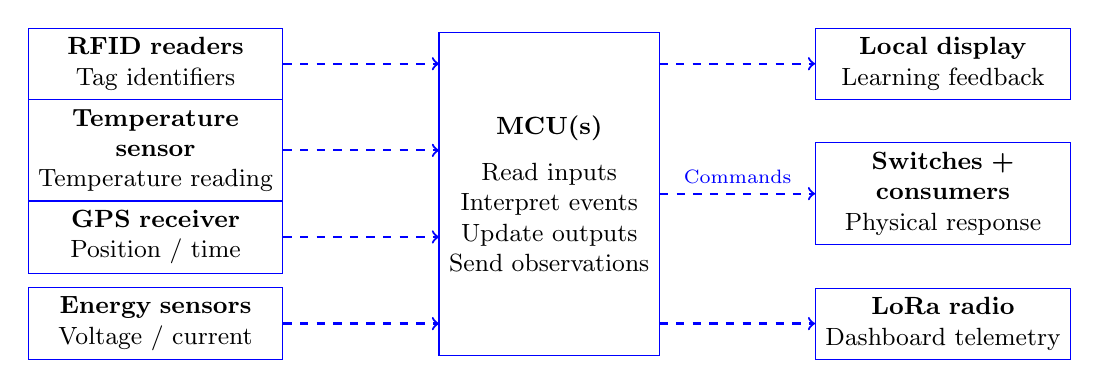
\begin{tikzpicture}[every node/.style={align=center,font=\small},peripheral/.style={draw=blue,text width=3cm,minimum height=.8cm}]
\node[peripheral] (rfid) at (0,0) {\textbf{RFID readers}\\Tag identifiers};
\node[peripheral] (temp) at (0,-1.1) {\textbf{Temperature sensor}\\Temperature reading};
\node[peripheral] (gps) at (0,-2.2) {\textbf{GPS receiver}\\Position / time};
\node[peripheral] (energy) at (0,-3.3) {\textbf{Energy sensors}\\Voltage / current};
\node[draw=blue,inner sep=0,minimum width=2.8cm,minimum height=4.1cm,text width=2.6cm] (mcu) at (5,-1.65) {\textbf{MCU(s)}\\[.6em]Read inputs\\Interpret events\\Update outputs\\Send observations};
\node[peripheral] (display) at (10,0) {\textbf{Local display}\\Learning feedback};
\node[peripheral] (loads) at (10,-1.65) {\textbf{Switches + consumers}\\Physical response};
\node[peripheral] (network) at (10,-3.3) {\textbf{LoRa radio}\\Dashboard telemetry};
\draw[->,thick,dashed,blue] (rfid.east)--(3.6,0);
\draw[->,thick,dashed,blue] (temp.east)--(3.6,-1.1);
\draw[->,thick,dashed,blue] (gps.east)--(3.6,-2.2);
\draw[->,thick,dashed,blue] (energy.east)--(3.6,-3.3);
\draw[->,thick,dashed,blue] (6.4,0)--(display.west);
\draw[->,thick,dashed,blue] (mcu.east)--node[above,font=\scriptsize]{Commands} (loads.west);
\draw[->,thick,dashed,blue] (6.4,-3.3)--(network.west);
\end{tikzpicture}
\end{center}
\begin{itemize}
    \item \textbf{Physical interaction and measurements meet at the MCU}; both can inform local feedback.
    \item \textbf{LoRaWAN and TTN carry the telemetry}; MQTT supplies the Pi backend and browser dashboard.
\end{itemize}
\vfill{\scriptsize Functional connections, not pin assignments. Telemetry path: LoRa radio, LoRaWAN gateway, TTN, then MQTT on the Pi; the local display is a separate output.}
\end{frame}

% Slide 25
\begin{frame}{Workshop Impressions -- 2026}{Three RFID Readers and Their Wiring}
\centering
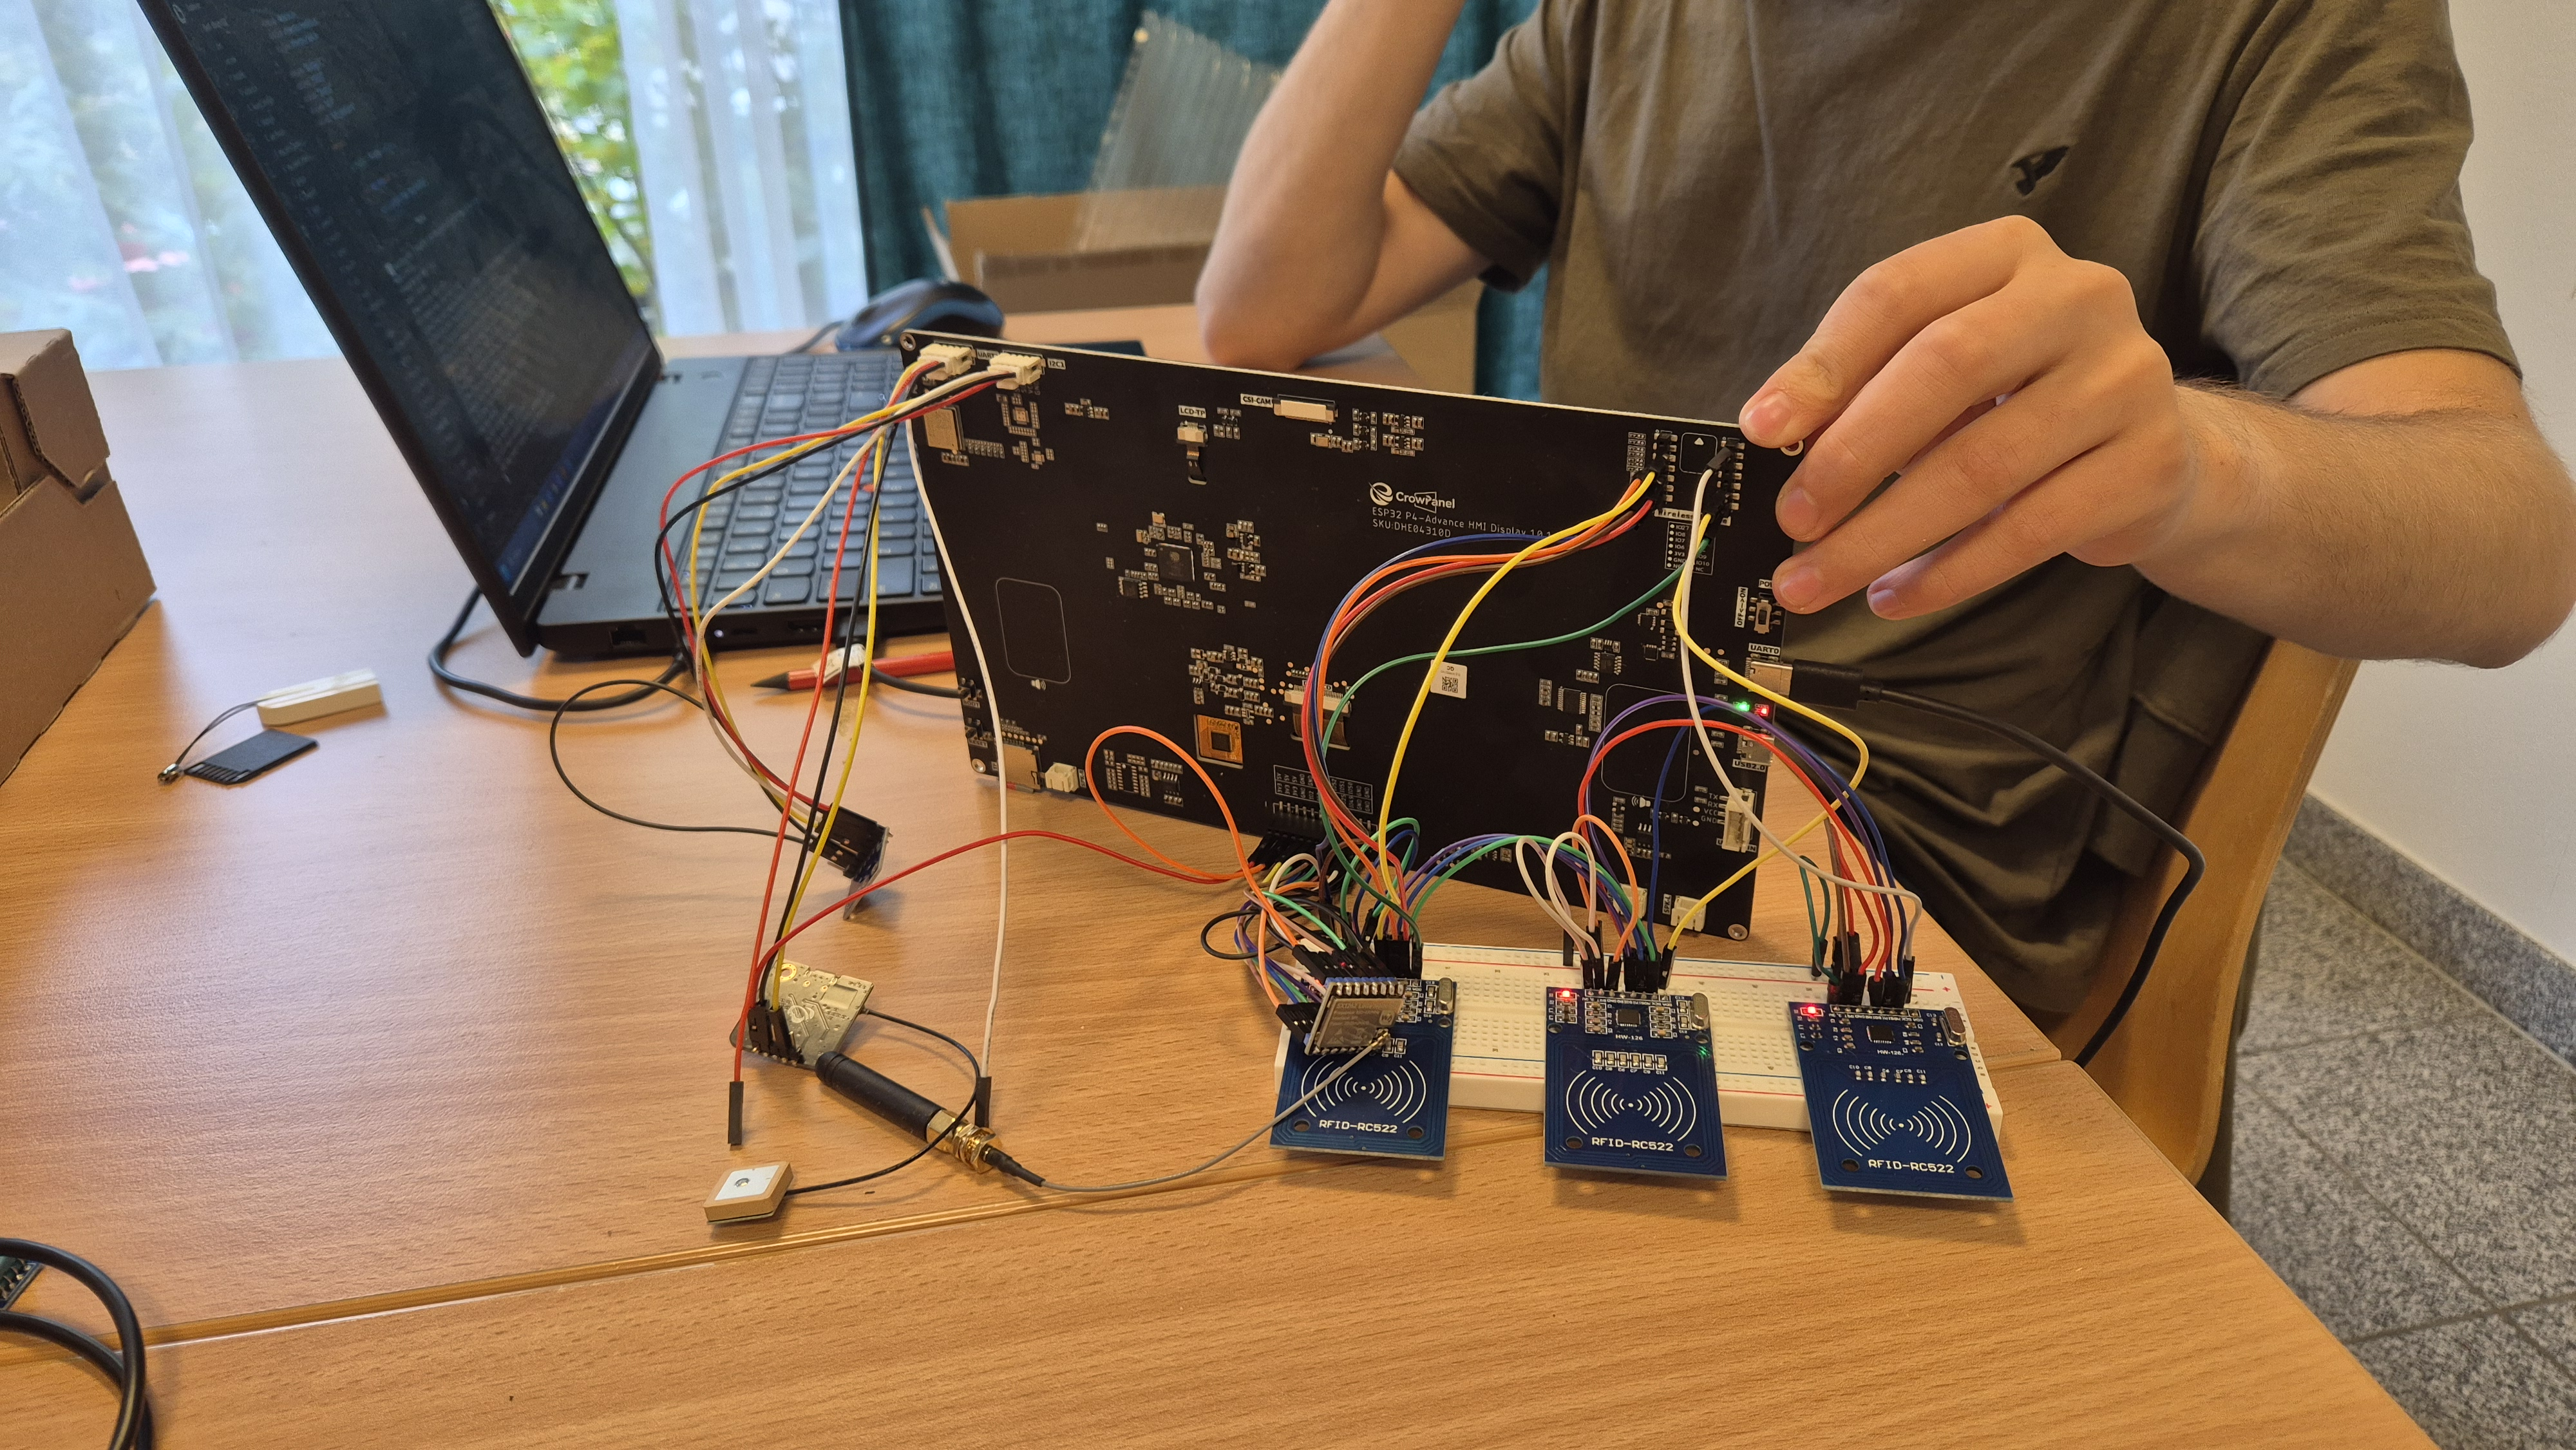
\includegraphics[width=\textwidth,height=.70\paperheight,keepaspectratio]{slides/035-ga-in-it-preintro/material/workshop-impressions-2026/20261029_111217.jpg}
\par\smallskip{\small Three RFID readers \quad$\cdot$\quad Breadboard connections \quad$\cdot$\quad Controller and display wiring}
\end{frame}

% Slide 26
\begin{frame}{Workshop Impressions -- 2026}{Connecting the Controller and Display}
\centering
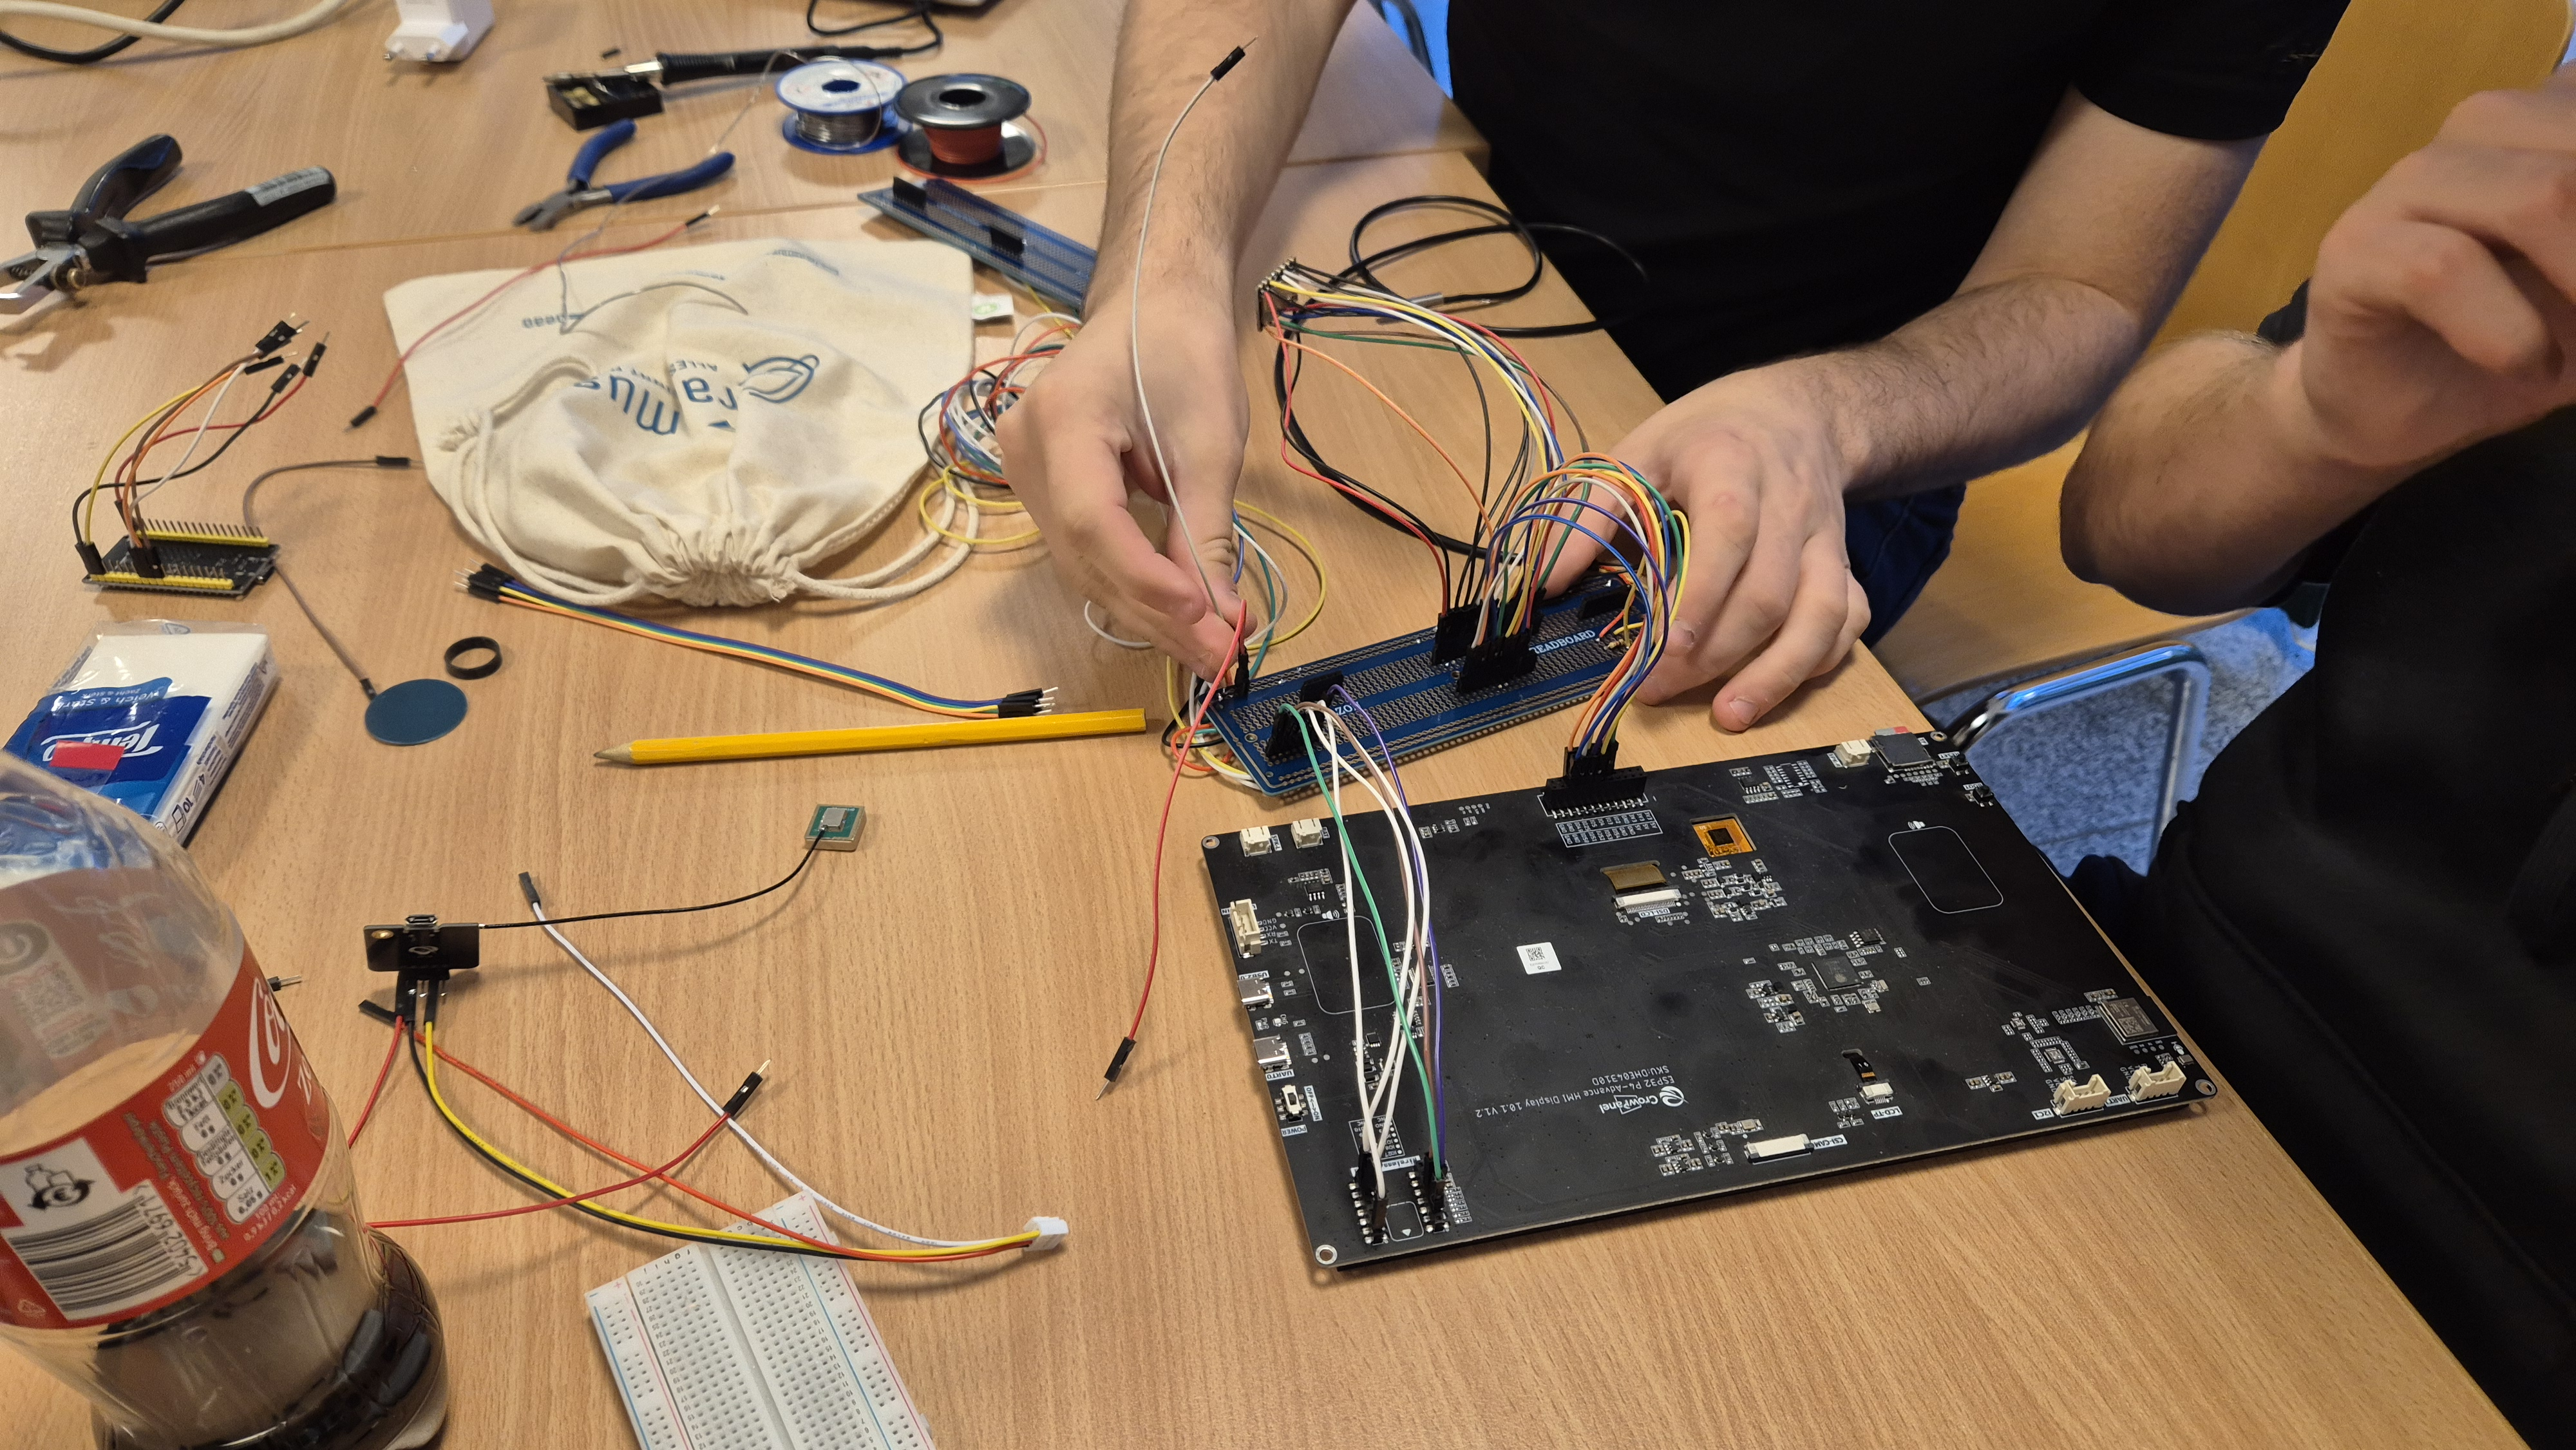
\includegraphics[width=\textwidth,height=.70\paperheight,keepaspectratio]{slides/035-ga-in-it-preintro/material/workshop-impressions-2026/20261103_152419.jpg}
\par\smallskip{\small Wiring \quad$\cdot$\quad Physical interfaces \quad$\cdot$\quad Integration}
\end{frame}

% Slide 27
\begin{frame}{Workshop Impressions -- 2026}{Behind the Panel: Integrating the Wiring}
\begin{columns}[c,onlytextwidth]
\column{.62\textwidth}\centering
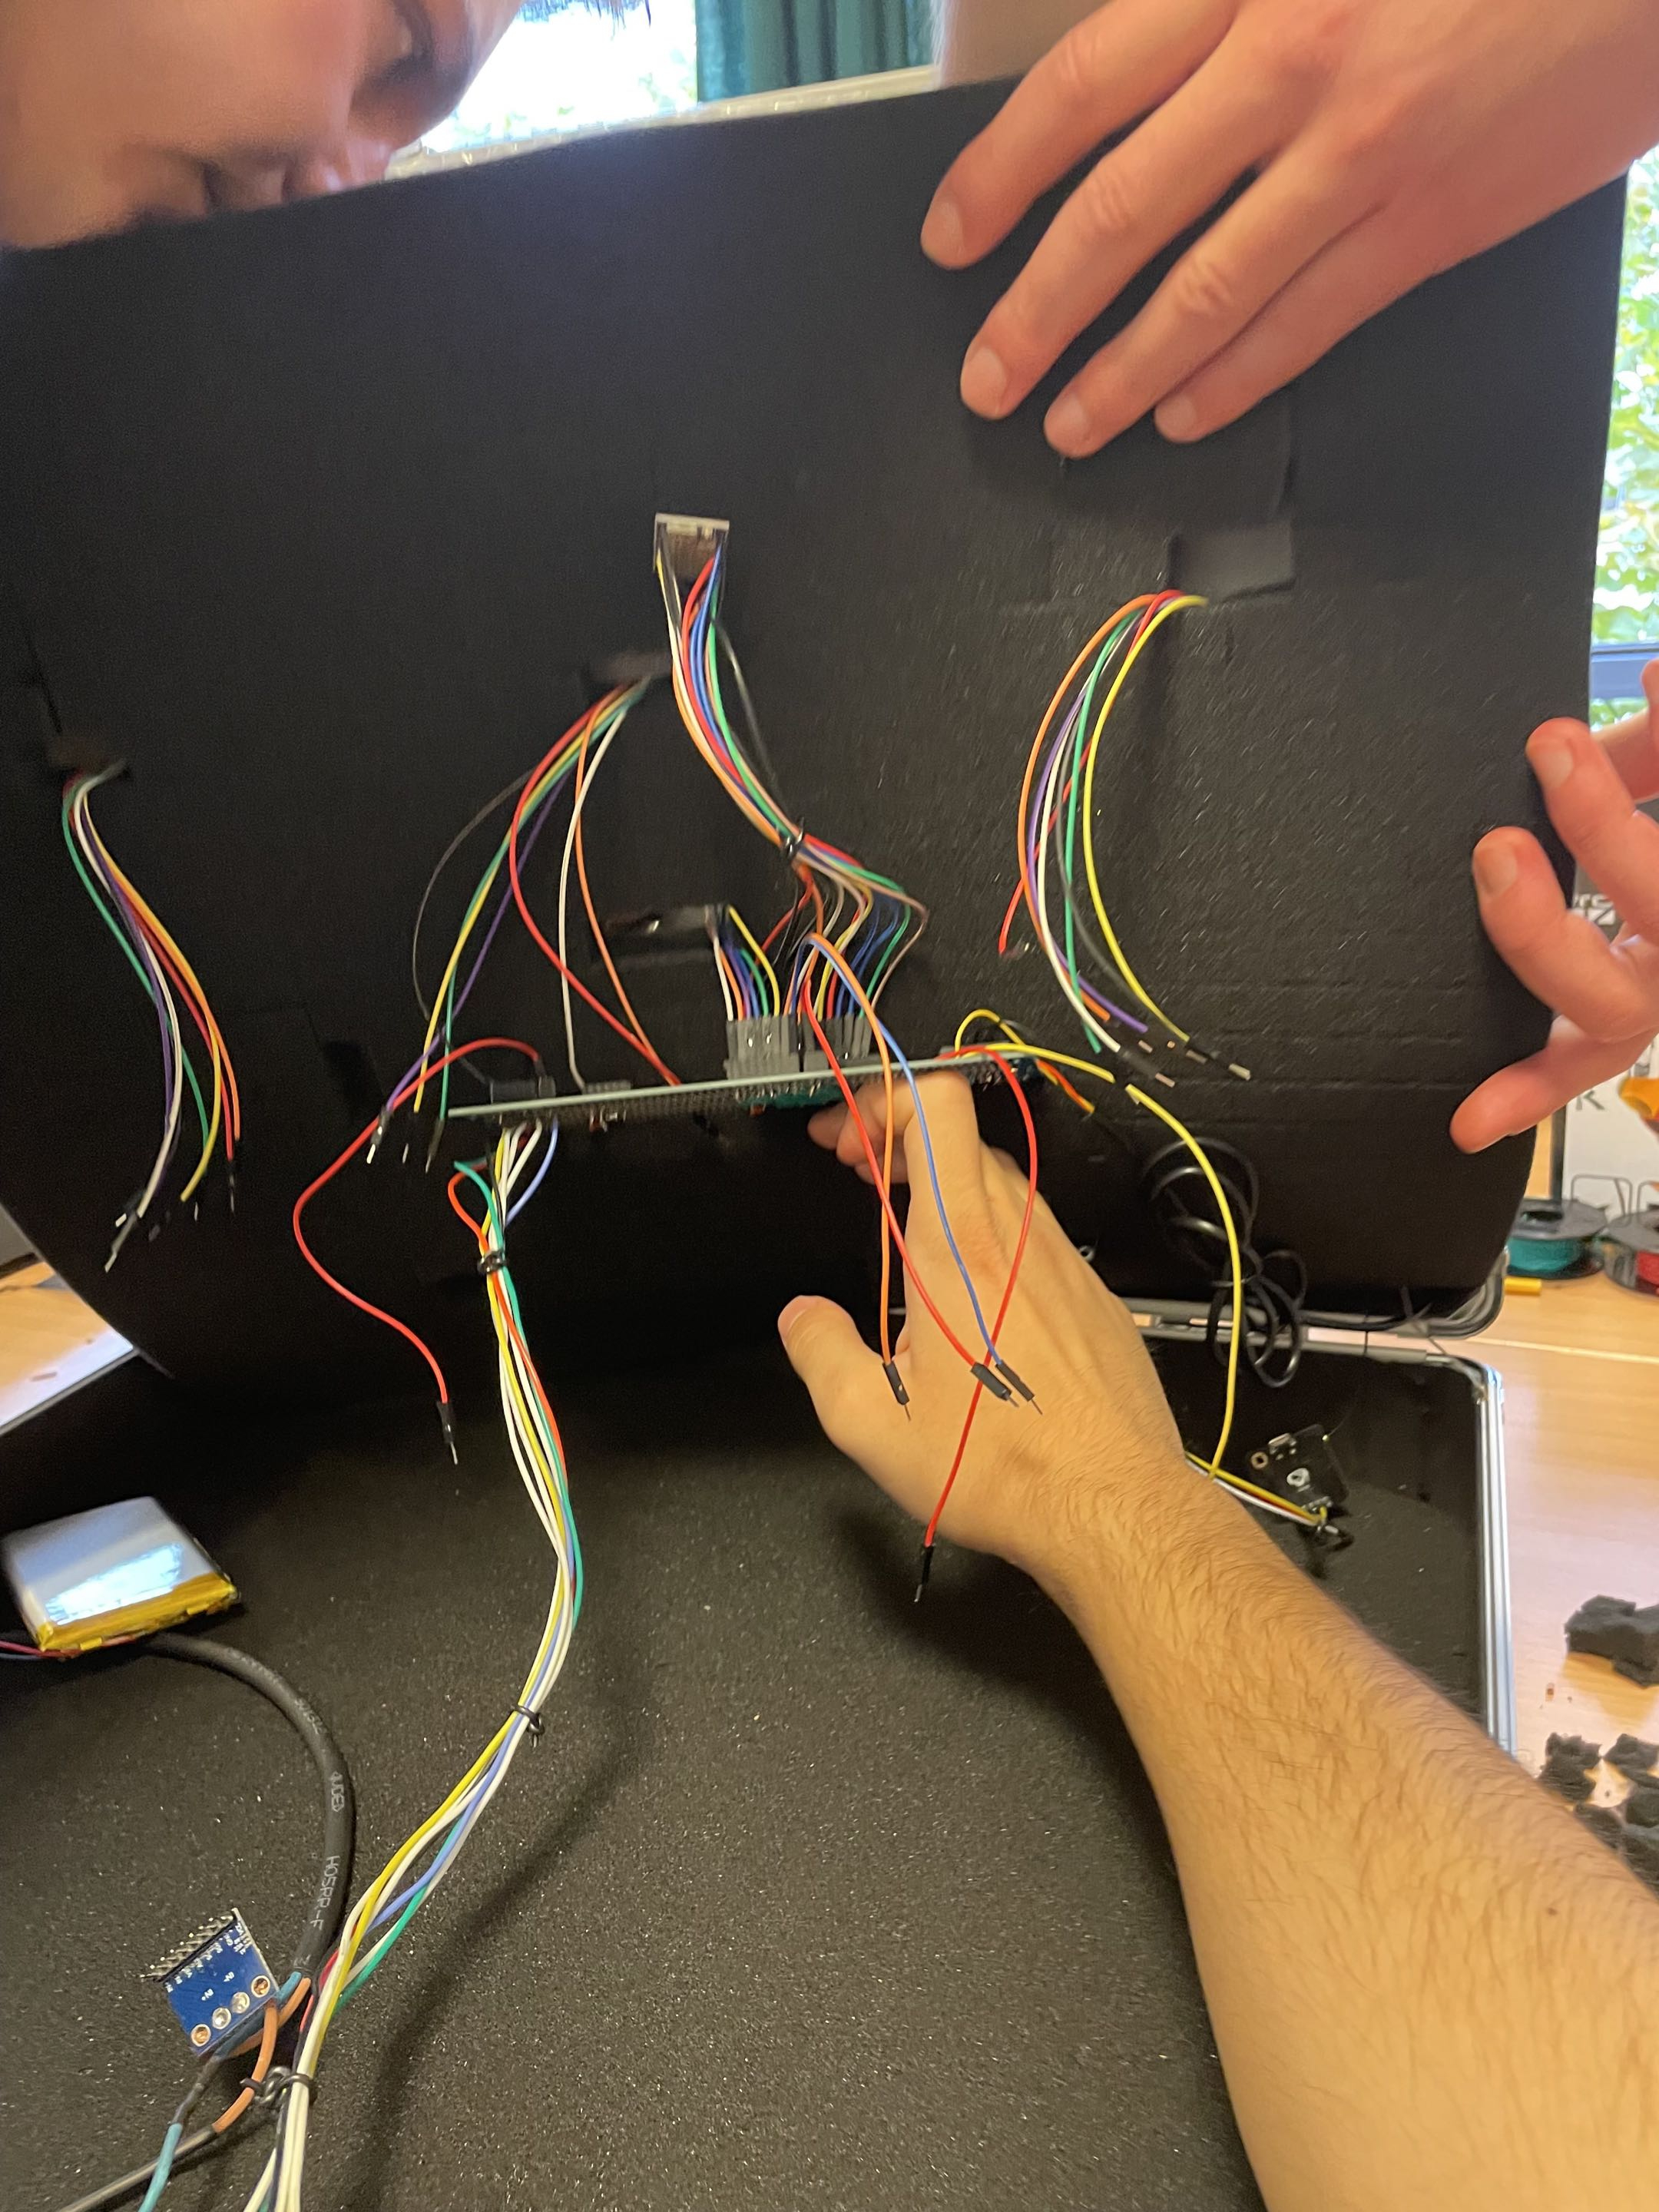
\includegraphics[width=\linewidth,height=.70\paperheight,keepaspectratio]{slides/036-sdg-story/material/workshop-impressions-2026/internal-panel-wiring.jpg}
\column{.34\textwidth}
\begin{itemize}
    \item \textbf{Internal connections} link the components.
    \item \textbf{Wiring behind the panel} becomes part of the physical assembly.
    \item \textbf{Integration in the case} brings the device together.
\end{itemize}
\end{columns}
\end{frame}

% Slide 28
\begin{frame}{Workshop Impressions -- 2026}{Fitting Solar Generation into the Device}
\begin{columns}[c,onlytextwidth]
\column{.62\textwidth}\centering
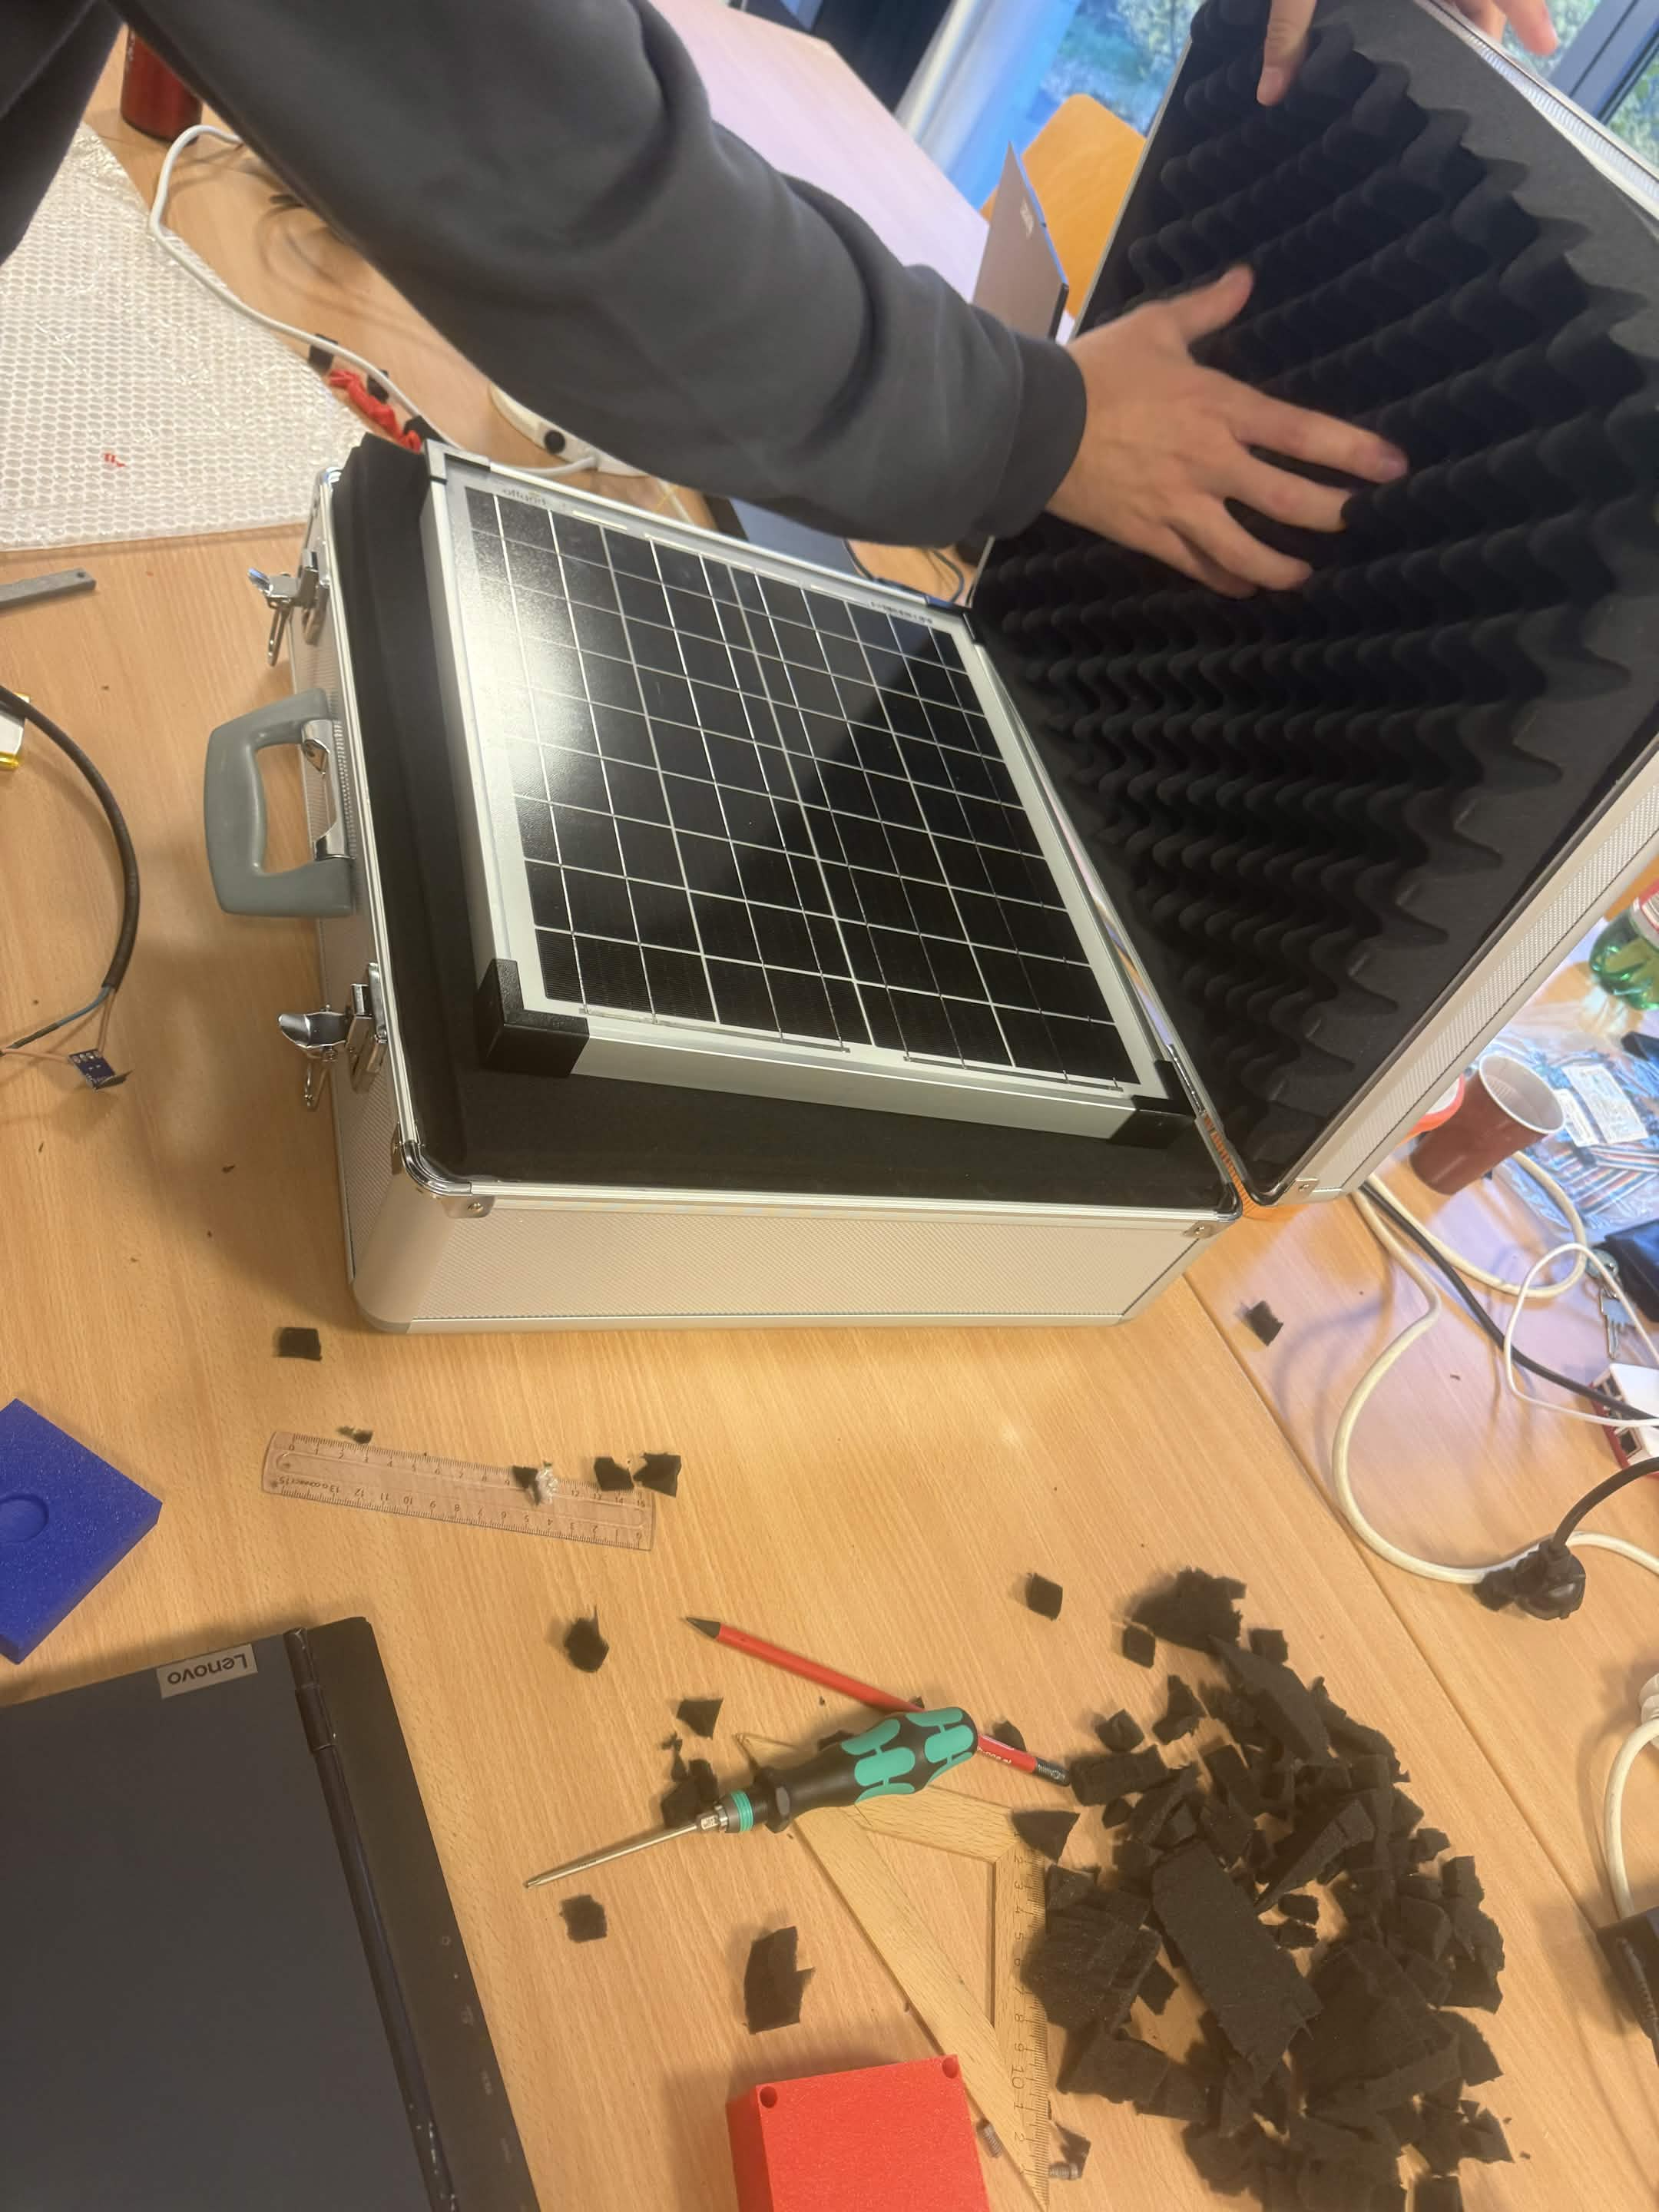
\includegraphics[width=\linewidth,height=.70\paperheight,keepaspectratio]{slides/035-ga-in-it-preintro/material/workshop-impressions-2026/IMG_6293.jpg}
\column{.34\textwidth}
\begin{itemize}
    \item \textbf{Solar panel} in the case.
    \item \textbf{Packaging} becomes part of the system.
    \item \textbf{Assembly} connects the learning idea with a physical device.
\end{itemize}
\end{columns}
\end{frame}

% Slide 29
\begin{frame}{Inside the Learning Device: A Small, Real Microgrid}{The Whole Device Must Fit the Energy Budget}
\begin{center}
\begin{tikzpicture}[every node/.style={align=center,font=\small},device/.style={draw=fh-ooe-red,text width=2.5cm,minimum height=.8cm}]
\node[device] (panel) at (0,0) {\textbf{Solar panel}};
\node[device] (ctrl) at (3.4,0) {\textbf{Charge controller}};
\node[device] (bus) at (6.8,0) {\textbf{Shared supply}};
\node[device] (loads) at (10.2,0) {\textbf{Consumers}};
\node[device] (bat) at (3.4,-1.65) {\textbf{Battery}};
\node[device] (mcu) at (6.8,-1.65) {\textbf{MCUs and peripherals}};
\node[device] (pi) at (10.2,-1.65) {\textbf{Pi and router}};
\draw[->,thick,fh-ooe-red] (panel.east)--(ctrl.west);
\draw[->,thick,fh-ooe-red] (ctrl.east)--(bus.west);
\draw[->,thick,fh-ooe-red] (bus.east)--(loads.west);
\draw[<->,thick,fh-ooe-red] (ctrl.south)--(bat.north);
\coordinate (supplybranch) at (6.8,-.85);
\draw[thick,fh-ooe-red] (bus.south)--(supplybranch);
\fill[fh-ooe-red] (supplybranch) circle (1.5pt);
\draw[->,thick,fh-ooe-red] (supplybranch)--(mcu.north);
\draw[->,thick,fh-ooe-red] (supplybranch)-|(pi.north);
\end{tikzpicture}
\end{center}
\vspace{.7em}
\begin{itemize}
    \item \textbf{Include every peripheral}: RFID readers, temperature and GPS modules, energy sensors, LoRa radio and the local display.
    \item \textbf{Include computation, networking and outputs}: MCUs, Raspberry Pi, router, switches and consumers.
    \item \textbf{Autonomy is a whole-device requirement}: the panel and battery must supply every included device.
\end{itemize}
\vfill{\scriptsize Power-flow overview, not a wiring diagram. Voltage conversion and protection depend on the design; data connections are shown separately.}
\end{frame}

% Slide 30
\begin{frame}{The Suitcase: From LoRaWAN to the Live Dashboard}{The Same Telemetry Path as the Buoy}
\begin{center}
\begin{tikzpicture}[every node/.style={align=center,font=\small},service/.style={draw=fh-ooe-red,text width=2cm,minimum height=.7cm}]
\draw[gray] (7.65,.72) rectangle (13.35,-3.45);
\node[font=\small\bfseries] at (10.5,1) {Raspberry Pi: local backend};
\node[service] (buoy) at (0,0) {Suitcase\\MCU};
\node[service] (gw) at (3,0) {LoRaWAN\\gateway};
\node[service] (ttn) at (6,0) {TTN\\Network service};
\node[service] (mqtt) at (9,0) {MQTT broker};
\node[service] (store) at (12,0) {Storage service};
\node[service] (db) at (12,-1.6) {MariaDB\\History};
\node[service] (dash) at (9,-2.85) {Dashboard server};
\node[service] (browser) at (5.3,-2.85) {Browser\\Live view};
\draw[->,thick,fh-ooe-red] (buoy.east)--(gw.west);
\draw[->,thick,fh-ooe-red] (gw.east)--(ttn.west);
\draw[->,thick,fh-ooe-red] (ttn.east)--(mqtt.west);
\draw[->,thick,fh-ooe-red] (mqtt.east)--(store.west);
\draw[->,thick,fh-ooe-red] (store.south)--(db.north);
\draw[->,thick,blue] (mqtt.south)-- node[left,font=\scriptsize]{Live readings} (dash.north);
\draw[->,thick,fh-ooe-red] (db.south)|-(dash.east);
\node[font=\scriptsize] at (11.2,-2.6) {History};
\draw[->,thick,blue] (dash.west)--node[above]{SSE} (browser.east);
\node[font=\scriptsize,align=left] at (1.2,-1.6) {\textcolor{fh-ooe-red}{Red: uplink / stored history}\\\textcolor{blue}{Blue: live readings / SSE}};
\end{tikzpicture}
\end{center}
\begin{itemize}
    \item \textbf{Suitcase uplinks go via LoRaWAN and TTN}; the Pi receives them through MQTT.
    \item \textbf{MariaDB holds history}; the server sends \textbf{live browser updates via SSE}.
    \item \textbf{Local display}: device feedback. \textbf{Browser dashboard}: observations received through TTN.
\end{itemize}
\vfill{\scriptsize Gateway and backend need internet access to TTN, even when the dashboard is hosted locally.}
\end{frame}


% Slide 31
\begin{frame}{One Action, One Visible Energy Lesson}{Shade the Panel -- Predict, Observe, Explain}
\begin{center}
\begin{tikzpicture}[every node/.style={align=center,font=\small,text width=2.9cm}]
\node (shade) at (0,0) {\textbf{Shade the panel}\\Change the conditions};
\node (generation) at (4,0) {\textbf{Less generation}\\Read the power};
\node (balance) at (8,0) {\textbf{Compare with demand}\\Is generation still enough?};
\draw[->,thick,fh-ooe-red] (shade)--(generation);
\draw[->,thick,fh-ooe-red] (generation)--(balance);
\end{tikzpicture}
\end{center}
\vspace{.6em}
\begin{itemize}
    \item \textbf{Predict}: will the consumers keep running, and where could their energy come from?
    \item \textbf{Observe}: the MCU sends measurements via LoRaWAN and TTN; MQTT and SSE bring them to the browser dashboard.
    \item \textbf{Explain}: if demand exceeds generation, an available battery can supply the difference.
    \item \textbf{Try again}: remove the shade or reduce demand and compare the responses.
\end{itemize}
\vfill
\alert{Generation, consumption and storage are connected -- the learner can investigate how.}
\par\smallskip{\scriptsize Possible learning activity. The response depends on battery state, available energy and the device's control behaviour.}
\end{frame}

% Slide 32
\begin{frame}{What Could a Beginner Discover?}{Gamification Gives Learning a Purpose and Feedback}
\small\renewcommand{\arraystretch}{1.5}
\par\noindent\begin{tabularx}{\textwidth}{@{}>{\raggedright\arraybackslash}p{.28\textwidth}>{\raggedright\arraybackslash}X>{\raggedright\arraybackslash}X@{}}
\toprule
\textbf{Possible exploration} & \textbf{What becomes visible?} & \textbf{What could a learner explain?}\\\midrule
Change the panel's illumination & Generation rises or falls & Available energy changes with conditions.\\
Compare supply and consumption & The battery charges or supplies energy & Storage moves energy from one time to another.\\
Add or prioritise consumers & Demand competes for limited supply & A microgrid needs choices about energy use.\\\bottomrule
\end{tabularx}\par
\vspace{.8em}
\normalsize\begin{itemize}
    \item A \textbf{challenge} gives a reason to explore; \textbf{feedback} connects action and consequence.
    \item Ask learners to \textbf{predict, try and explain} what changed.
    \item These are \textbf{possible activities}; students define and evaluate the learning experience.
\end{itemize}
\end{frame}

\part[nopartpage]{Contribution and Evidence}
% Slide 33
\begin{frame}{Three Years, One Common Approach}{From a Sustainability Challenge to a Contribution We Can Examine}
\small\renewcommand{\arraystretch}{1.35}
\par\noindent\begin{tabularx}{\textwidth}{@{}>{\raggedright\arraybackslash}p{.07\textwidth}>{\raggedright\arraybackslash}p{.18\textwidth}>{\raggedright\arraybackslash}X>{\raggedright\arraybackslash}X>{\raggedright\arraybackslash}X@{}}
\toprule
\textbf{Year} & \textbf{SDG connection} & \textbf{Project contribution} & \textbf{Role of IoT} & \textbf{Evidence to seek}\\\midrule
2024 & Ecosystems and invasive species: 6.6 / 15.8 & A buoy prototype for environmental observation & Connect physical conditions with measurements & Reliable readings that answer research questions\\
2025 & Same ecosystem challenge: 6.6 / 15.8 & An integrated water-monitoring system & Bring devices, data and interfaces together & Usable information and examples of decisions it supports\\
2026 & Energy and sustainability learning: 7.2 / 4.7 & A gamified microgrid learning device & Make physical energy choices observable & What beginners can explain; what the system can demonstrate\\\bottomrule
\end{tabularx}\par
\vspace{.9em}
\normalsize\textbf{Buoy:} support environmental investigation.\quad
\textbf{Learning device:} develop energy literacy.\par
\vspace{.4em}\alert{Each needs evidence of usefulness beyond a working prototype.}
\vfill
{\scriptsize Targets: \href{https://sdgs.un.org/goals/goal6}{6.6}, \href{https://sdgs.un.org/goals/goal15}{15.8}, \href{https://sdgs.un.org/goals/goal7}{7.2}, \href{https://sdgs.un.org/goals/goal4}{4.7}. Connections are an interpretation of the project purposes.}
\end{frame}

% Slide 34
\begin{frame}{Who Benefits -- and How Would We Know?}{Apply the Same Questions to a Project You Know}
\begin{enumerate}
    \item \textbf{Who benefits?} Name the people or ecosystem and the need you are addressing.
    \item \textbf{What changes?} Explain the intended improvement and the SDG target it relates to.
    \item \textbf{How would you know?} Suggest one observation that would show progress.
    \item \textbf{What could go wrong?} Consider maintenance, energy use, waste or unequal access.
\end{enumerate}
\vspace{1em}
\alert{Choose one example. Explain the benefit and the evidence -- in one minute.}
\vfill
{\large The sustainability purpose guides the project. Technology helps us pursue it.}
\par\vspace{.7em}
{\tiny SDG icons: United Nations, \href{https://www.un.org/sustainabledevelopment/}{un.org/sustainabledevelopment}. The content of this publication has not been approved by the United Nations and does not reflect the views of the United Nations or its officials or Member States.}
\end{frame}
